\documentclass[runningheads,plain]{llncs}

\usepackage[T1]{fontenc}
\usepackage{lmodern}
\usepackage{amssymb,amsmath,stmaryrd,enumerate}
\usepackage{ifxetex,ifluatex}
\usepackage{xspace}

\usepackage{xcolor}
\newcommand{\erase}[1]{\textcolor{orange}{#1}}


\usepackage{fixltx2e} % provides \textsubscript
% use upquote if available, for straight quotes in verbatim environments

% lncs 
\usepackage{makeidx}
%\institute{University of Groningen, The Netherlands, \\ \texttt{}}

\providecommand{\tightlist}{%
  \setlength{\itemsep}{0pt}\setlength{\parskip}{0pt}}

\IfFileExists{upquote.sty}{\usepackage{upquote}}{}
\ifnum 0\ifxetex 1\fi\ifluatex 1\fi=0 % if pdftex
  \usepackage[utf8]{inputenc}
\else % if luatex or xelatex
  \ifxetex
    \usepackage{mathspec}
    \usepackage{xltxtra,xunicode}
  \else
    \usepackage{fontspec}
  \fi
  \defaultfontfeatures{Mapping=tex-text,Scale=MatchLowercase}
  \newcommand{\euro}{€}
\fi
% use microtype if available
\IfFileExists{microtype.sty}{\usepackage{microtype}}{}
\usepackage{color}
\usepackage{fancyvrb}
\newcommand{\VerbBar}{|}
\newcommand{\VERB}{\Verb[commandchars=\\\{\}]}
\DefineVerbatimEnvironment{Highlighting}{Verbatim}{commandchars=\\\{\}}
% Add ',fontsize=\small' for more characters per line
\newenvironment{Shaded}{}{}
\newcommand{\KeywordTok}[1]{\textcolor[rgb]{0.00,0.44,0.13}{\textbf{#1}}}
\newcommand{\DataTypeTok}[1]{\textcolor[rgb]{0.56,0.13,0.00}{#1}}
\newcommand{\DecValTok}[1]{\textcolor[rgb]{0.25,0.63,0.44}{#1}}
\newcommand{\BaseNTok}[1]{\textcolor[rgb]{0.25,0.63,0.44}{#1}}
\newcommand{\FloatTok}[1]{\textcolor[rgb]{0.25,0.63,0.44}{#1}}
\newcommand{\ConstantTok}[1]{\textcolor[rgb]{0.53,0.00,0.00}{#1}}
\newcommand{\CharTok}[1]{\textcolor[rgb]{0.25,0.44,0.63}{#1}}
\newcommand{\SpecialCharTok}[1]{\textcolor[rgb]{0.25,0.44,0.63}{#1}}
\newcommand{\StringTok}[1]{\textcolor[rgb]{0.25,0.44,0.63}{#1}}
\newcommand{\VerbatimStringTok}[1]{\textcolor[rgb]{0.25,0.44,0.63}{#1}}
\newcommand{\SpecialStringTok}[1]{\textcolor[rgb]{0.73,0.40,0.53}{#1}}
\newcommand{\ImportTok}[1]{#1}
\newcommand{\CommentTok}[1]{\textcolor[rgb]{0.38,0.63,0.69}{\textit{#1}}}
\newcommand{\DocumentationTok}[1]{\textcolor[rgb]{0.73,0.13,0.13}{\textit{#1}}}
\newcommand{\AnnotationTok}[1]{\textcolor[rgb]{0.38,0.63,0.69}{\textbf{\textit{#1}}}}
\newcommand{\CommentVarTok}[1]{\textcolor[rgb]{0.38,0.63,0.69}{\textbf{\textit{#1}}}}
\newcommand{\OtherTok}[1]{\textcolor[rgb]{0.00,0.44,0.13}{#1}}
\newcommand{\FunctionTok}[1]{\textcolor[rgb]{0.02,0.16,0.49}{#1}}
\newcommand{\VariableTok}[1]{\textcolor[rgb]{0.10,0.09,0.49}{#1}}
\newcommand{\ControlFlowTok}[1]{\textcolor[rgb]{0.00,0.44,0.13}{\textbf{#1}}}
\newcommand{\OperatorTok}[1]{\textcolor[rgb]{0.40,0.40,0.40}{#1}}
\newcommand{\BuiltInTok}[1]{#1}
\newcommand{\ExtensionTok}[1]{#1}
\newcommand{\PreprocessorTok}[1]{\textcolor[rgb]{0.74,0.48,0.00}{#1}}
\newcommand{\AttributeTok}[1]{\textcolor[rgb]{0.49,0.56,0.16}{#1}}
\newcommand{\RegionMarkerTok}[1]{#1}
\newcommand{\InformationTok}[1]{\textcolor[rgb]{0.38,0.63,0.69}{\textbf{\textit{#1}}}}
\newcommand{\WarningTok}[1]{\textcolor[rgb]{0.38,0.63,0.69}{\textbf{\textit{#1}}}}
\newcommand{\AlertTok}[1]{\textcolor[rgb]{1.00,0.00,0.00}{\textbf{#1}}}
\newcommand{\ErrorTok}[1]{\textcolor[rgb]{1.00,0.00,0.00}{\textbf{#1}}}
\newcommand{\NormalTok}[1]{#1}
\ifxetex
  \usepackage[setpagesize=false, % page size defined by xetex
              unicode=false, % unicode breaks when used with xetex
              xetex]{hyperref}
\else
  \usepackage[unicode=true]{hyperref}
\fi
\hypersetup{breaklinks=true,
            bookmarks=true,
            pdfauthor={Folkert de Vries \& Jorge A. Pérez},
            pdftitle={Reversible Session-Based Concurrency in Haskell},
            colorlinks=true,
            citecolor=blue,
            urlcolor=blue,
            linkcolor=magenta,
            pdfborder={0 0 0}}
\urlstyle{same}  % don't use monospace font for urls
%\setlength{\parindent}{0pt}
%\setlength{\parskip}{6pt plus 2pt minus 1pt}
%\setlength{\emergencystretch}{3em}  % prevent overfull lines
%\setcounter{secnumdepth}{5}

%\date{}
\usepackage{graphicx}
\usepackage{hyperref}
\usepackage[toc,page]{appendix}
\newcommand{\hideFromPandoc}[1]{#1}
\hideFromPandoc{ \let\Begin\begin \let\End\end }

%%%%%%%%%%%%%%%%%%%%%%%%%%%%%%%%%%%%%%%%%%%%%%%%%%%%%%%%%%%%%%%%%%%%%%%%%%%%%%%%%%%%%%%%%%%%%%%%%%%%
% Contents
% --------

% 1.  Formating
% 2.  Maths - Theorems
% 3.  The pi Calculus
% 4.  Session Syntax
% 5.  Subject Reduction
% 6.  Global Session Types
% 7.  Global Session Types Equivalence
% 8.  Projection
% 9.  Local Session Types
% 10. Behavioural Theory
% 11. Typed Transitions - Reductions
% 12. Typed Relations
% 13. Confluence Determinacy
% 14. Mapping
% 15. pi Constructs
% 16. LN Transform
% 17. General Types Processes Names Sessions ETC
% 18. newtheorem - newenvironment
% 19. Misc
%%%%%%%%%%%%%%%%%%%%%%%%%%%%%%%%%%%%%%%%%%%%%%%%%%%%%%%%%%%%%%%%%%%%%%%%%%%%%%%%%%%%%%%%%%%%%%%%%%%%


%%%%%%%%%%%%%%%%%%%%%%%%%%%%%%%%%%%%%%%%%%%%%%%%%%%%%%%%%%%%%%%%%%%%%%%%%%%%%%%%%%%%%%%%%%%%%%%%%%%%
%                                       FORMATING
%%%%%%%%%%%%%%%%%%%%%%%%%%%%%%%%%%%%%%%%%%%%%%%%%%%%%%%%%%%%%%%%%%%%%%%%%%%%%%%%%%%%%%%%%%%%%%%%%%%%

% Symbols
\newcommand{\semicolon}{:}
%\newcommand{\colon}{;}
\newcommand{\lrangle}[1]{\langle #1 \rangle}
\newcommand{\blrangle}[1]{\big\langle #1 \big\rangle}

%Tags
\newcommand{\parenthtext}[1]{(\textrm{\small #1})}
\newcommand{\brtext}[1]{[\textrm{\small #1}]}
\newcommand{\textinmath}[1]{\textrm{#1}}
\newcommand{\srule}[1]{\parenthtext{#1}}
\newcommand{\strule}[1]{\textrm{#1}}
\newcommand{\stypes}[1]{{\footnotesize \parenthtext{#1}}}
\newcommand{\ltsrule}[1]{{\footnotesize \lrangle{\textrm{#1}}}}
\newcommand{\eltsrule}[1]{{\footnotesize [\textrm{#1}]}}
\newcommand{\trule}[1]{{\footnotesize\brtext{#1}}}
\newcommand{\orule}[1]{{\scriptsize{\brtext{#1}}}}
\newcommand{\mrule}[1]{{\footnotesize{\parenthtext{#1}}}}

\newcommand{\iftag}{{\textrm{if }}}

% General
\newcommand{\noi}{\noindent}
\newcommand{\Hline}{\rule{\linewidth}{.5pt}}
\newcommand{\Hlinefig}{\rule{\linewidth}{.5pt}\vspace{-4mm}}
\newcommand{\myparagraph}[1]{\noindent{\textbf{#1}\ }}
\newcommand{\jparagraph}[1]{\paragraph{\textbf{#1}}}

%%%%%%%%%%%%%%%%%%%%%%%%%%%%%%%%%%%%%%%%%%%%%%%%%%%%%%%%%%%%%%%%%%%%%%%%%%%%%%%%%%%%%%%%%%%%%%%%%%%%
%                                       MATHS - THEOREMS
%%%%%%%%%%%%%%%%%%%%%%%%%%%%%%%%%%%%%%%%%%%%%%%%%%%%%%%%%%%%%%%%%%%%%%%%%%%%%%%%%%%%%%%%%%%%%%%%%%%%

%\newtheorem{notation}[definition]{Notation}

% BNF form
\newcommand{\bnfis}{\;\;::=\;\;}
%\newcommand{\bnfbar}{\;\;\;{\large |}\;\;\;}
%\newcommand{\sbnfbar}{\;|\;}
\def\bnfbar{\; \mbox{\large{$\parallel$}}\;}
\def\sbnfbar{\;\mbox{\large{$\mid$}}\;}


% Proof
\newcommand{\Case}[1]{\noi {\bf Case: }#1\\}
\newcommand{\proofend}{\qed}
%\newcommand{\proofend}{}
\newcommand{\Proof}{\noi {\bf Proof: }}

% Logic
\newcommand{\LogAnd}{\texttt{ and }}
\newcommand{\LogOr}{\texttt{ or }}

% Induction

\newcommand{\basic}{\noi {\bf Basic Step:}\\}
\newcommand{\inductive}{\noi {\bf Inductive Hypothesis:}\\}
\newcommand{\induction}{\noi {\bf Induction Step:}\\}

% Tree

\newcommand{\tree}[2]{
\ensuremath{\displaystyle
		\frac
		{
			%%\raisebox{0.0mm}{$\displaystyle{#1}$}
			#1
			%\vspace{0mm}
		}{
			%\vspace{2mm}
			#2
			%\raisebox{-0.4mm}{$\displaystyle{#2}$}
		}
	}
}


%\newcommand{\tree}[2]{
%\begin{prooftree}
%	#1
%	\justifies
%	#2
%\end{prooftree}
%}

\newcommand{\treeusing}[3]{
\begin{prooftree}
	#1
	\justifies
	#2
	\using
	#3
\end{prooftree}}

% Vectors
\newcommand{\vect}[1]{\tilde{#1}}
\newcommand{\mytilde}[1]{\widetilde{#1}}

% Functions - Set theory
\newcommand{\set}[1]{\{#1\}}
\newcommand{\es}{\emptyset}
\newcommand{\maxset}[1]{\max(#1)}
\newcommand{\setbar}{\ \ |\ \ }
\newcommand{\tuple}[2]{(#1, #2)}
\newcommand{\suchthat}{\cdot}
\newcommand{\powerset}[1]{\mathcal{P}(#1)}
\newcommand{\product}{\times}

\newcommand{\eval}{\downarrow}

\newcommand{\setsubtr}[2]{#1 \backslash #2}

\newcommand{\func}[2]{#1(#2)}
\newcommand{\dom}[1]{\mathtt{dom}(#1)}
\newcommand{\codom}[1]{\mathtt{codom}(#1)}

\newcommand{\funcbr}[2]{#1\lrangle{#2}}

\newcommand{\entails}{\text{implies}}


%%%%%%%%%%%%%%%%%%%%%%%%%%%%%%%%%%%%%%%%%%%%%%%%%%%%%%%%%%%%%%%%%%%%%%%%%%%%%%%%%%%%%%%%%%%%%%%%%%%%
%                                        pi - CALCULUS
%%%%%%%%%%%%%%%%%%%%%%%%%%%%%%%%%%%%%%%%%%%%%%%%%%%%%%%%%%%%%%%%%%%%%%%%%%%%%%%%%%%%%%%%%%%%%%%%%%%%

% Free-Bound notation
\newcommand{\freev}[1]{\lrangle{#1}}
\newcommand{\boundv}[1]{(#1)}

% General pi calculus Syntax
\newcommand{\send}[1]{\overline{#1}}
\newcommand{\ol}[1]{\overline{#1}}
\newcommand{\receive}[1]{#1.}
\newcommand{\inact}{\mathbf{0}}
\newcommand{\If}{\sessionfont{if}\ }
\newcommand{\Then}{\sessionfont{then}\ }
\newcommand{\Else}{\sessionfont{else}\ }
\newcommand{\ifthen}[2]{\If #1\ \Then #2\ }
\newcommand{\ifthenelse}[3]{\ifthen{#1}{#2} \Else #3}
\newcommand{\Par}{\;|\;}
\newcommand{\news}[1]{(\nu\, #1)}
\newcommand{\newsp}[2]{(\nu\, #1)(#2)}
\newcommand{\varp}[1]{#1}
%\newcommand{\rvar}[1]{\mathcal{#1}}
\newcommand{\rvar}[1]{#1}
%\newcommand{\rec}[2]{\mu #1. #2}
\newcommand{\recp}[2]{\mu \rvar{#1}. #2}

\newcommand{\Def}{\sessionfont{def}\ }

\newcommand{\defeq}{\stackrel{\Def}{=}}

\newcommand{\repl}{\ast\,}
\newcommand{\parcomp}[2]{\prod_{#1}{#2}}

% Free-Bound-Names sets
\newcommand{\bn}[1]{\mathtt{bn}(#1)}
\newcommand{\fn}[1]{\mathtt{fn}(#1)}
\newcommand{\sn}[1]{\mathtt{sn}(#1)}
\newcommand{\ofn}[1]{\mathsf{ofn}(#1)}
\newcommand{\fv}[1]{\mathtt{fv}(#1)}
\newcommand{\bv}[1]{\mathtt{bv}(#1)}
\newcommand{\fs}[1]{\mathtt{fs}(#1)}
\newcommand{\fpv}[1]{\mathtt{fpv}(#1)}
\newcommand{\nam}[1]{\mathtt{n}(#1)}

%Subject - Object
\newcommand{\subj}[1]{\mathtt{subj}(#1)}
\newcommand{\obj}[1]{\mathtt{obj}(#1)}

% Relations
\newcommand{\relfont}[1]{\mathcal{#1}}
\newcommand{\rel}[3]{#1\ \relfont{#2}\ #3}

\newcommand{\scong}{\equiv}
\newcommand{\acong}{\scong_{\alpha}}
\newcommand{\wb}{\approx}
\newcommand{\fwb}{\approx^\mathtt{C}}
\newcommand{\hwb}{\approx^\mathtt{H}}
\newcommand{\swb}{\approx^{s}}
\newcommand{\wbc}{\approx}
\newcommand{\WB}{\approx}

\newcommand{\red}{\longrightarrow}
\newcommand{\Red}{\rightarrow\!\!\!\!\!\rightarrow}
\newcommand{\Redleft}{\leftarrow\!\!\!\!\!\leftarrow}

%\newcommand{\subst}[2]{\set{#1/#2 }}
\def\subst#1#2{\{\raisebox{.5ex}{\small$#1$}\! / \mbox{\small$#2$}\}}

% Context
\newcommand{\hole}{-}
\newcommand{\context}[2]{#1[#2]}
\newcommand{\Ccontext}[1]{\C[#1]}

% Expression Context
\newcommand{\Econtext}[1]{\E[#1]}

% Barbs
\newcommand{\barb}[1]{\downharpoonright_{#1}}
\newcommand{\Barb}[1]{\Downarrow_{#1}}
\newcommand{\nbarb}[1]{\not\downarrow_{#1}}
\newcommand{\nBarb}[1]{\not\Downarrow_{#1}}

% General
%\newcommand{\ESP}{\ensuremath{\mathbf{ESP}}}
\newcommand{\ESP}{\text{ESP}}
\newcommand{\ESPsel}{\ESP^+}

%%%%%%%%%%%%%%%%%%%%%%%%%%%%%%%%%%%%%%%%%%%%%%%%%%%%%%%%%%%%%%%%%%%%%%%%%%%%%%%%%%%%%%%%%%%%%%%%%%%%
%                                        SESSION SYNTAX
%%%%%%%%%%%%%%%%%%%%%%%%%%%%%%%%%%%%%%%%%%%%%%%%%%%%%%%%%%%%%%%%%%%%%%%%%%%%%%%%%%%%%%%%%%%%%%%%%%%%

% Session font
\newcommand{\sessionfont}[1]{\mathtt{#1}}
\newcommand{\vart}[1]{\mathsf{#1}}

% General Session symbols
\newcommand{\ssep}{;}
\newcommand{\shsep}{.}
\newcommand{\outses}{!}
\newcommand{\inpses}{?}
\newcommand{\selses}{\triangleleft}
\newcommand{\brases}{\triangleright}
\newcommand{\dual}[1]{\overline{#1}}
\newcommand{\cat}{\cdot}

\newcommand{\allstypes}{\mathcal{S}}

% Binary Session Syntax


\newcommand{\bacc}[2]{#1 \boundv{#2} \shsep}
\newcommand{\breq}[2]{\send{#1} \freev{#2} \shsep}
\newcommand{\bareq}[2]{\send{#1} \freev{#2}}

\newcommand{\breqt}[3]{\send{#1} \boundv{#2:#3} \shsep}
\newcommand{\bacct}[3]{#1 \boundv{#2:#3} \shsep}

\newcommand{\bout}[2]{#1 \outses \freev{#2} \shsep}
\newcommand{\bbout}[2]{#1 \outses \blrangle{#2} \shsep}
\newcommand{\binp}[2]{#1 \inpses \boundv{#2} \shsep}
\newcommand{\bselold}[2]{#1 \selses #2 \shsep}
\newcommand{\bsel}[2]{#1 \selses \set{#2}}

%\newcommand{\bout}[2]{#1 \outses \freev{#2} \ssep}
%\newcommand{\bbout}[2]{#1 \outses \blrangle{#2} \ssep}
%\newcommand{\binp}[2]{#1 \inpses \boundv{#2} \ssep}
%\newcommand{\bsel}[2]{#1 \selses #2 \ssep}
\newcommand{\bbra}[2]{#1 \brases \set{#2}}
\newcommand{\bbras}[2]{#1 \brases #2}
\newcommand{\bbraP}[1]{#1 \brases \lPi}

% Multiparty Session syntax

\newcommand{\role}[1]{[#1]}

\newcommand{\srole}[2]{#1\role{#2}}
\newcommand{\sqrole}[2]{#1^{[]}\role{#2}}

\newcommand{\fromto}[2]{\role{#1} \role{#2}}
\newcommand{\sfromto}[3]{#1\fromto{#2}{#3}}

\newcommand{\sout}[3]{\srole{#1}{#2} \outses \freev{#3} \ssep}
\newcommand{\sinp}[3]{\srole{#1}{#2} \inpses \boundv{#3} \ssep}
\newcommand{\sdel}[4]{\srole{#1}{#2} \outses \freev{\srole{#3}{#4}} \ssep}
\newcommand{\ssel}[3]{\srole{#1}{#2} \selses #3 \ssep}
\newcommand{\sbra}[3]{\srole{#1}{#2} \brases \set{#3}}
\newcommand{\sbras}[3]{\srole{#1}{#2} \brases #3}
\newcommand{\sbraP}[2]{\srole{#1}{#2} \brases \lPi}

\newcommand{\acc}[3]{#1 \role{#2} \boundv{#3} \shsep}
\newcommand{\req}[3]{\send{#1} \role{#2} \boundv{#3} \shsep}
\newcommand{\areq}[3]{\send{#1} \role{#2} \freev{#3}}

\newcommand{\out}[4]{\sfromto{#1}{#2}{#3} \outses \freev{#4} \ssep}
\newcommand{\inp}[4]{\sfromto{#1}{#2}{#3} \inpses \boundv{#4} \ssep}
\newcommand{\del}[5]{\sfromto{#1}{#2}{#3} \outses \freev{\srole{#4}{#5}} \ssep}
\newcommand{\sel}[4]{\sfromto{#1}{#2}{#3} \selses #4 \ssep}
\newcommand{\bra}[4]{\sfromto{#1}{#2}{#3} \brases \set{#4}}
\newcommand{\bras}[4]{\sfromto{#1}{#2}{#3} \brases #4}
\newcommand{\braP}[3]{\sfromto{#1}{#2}{#3} \brases \lPi}

% Arrive construct
\newcommand{\arrivetext}{\mathtt{arrive}}
\newcommand{\arrive}[1]{\arrivetext\ #1}
\newcommand{\arrivem}[2]{\arrivetext\ #1\ #2}

% Typecase construct
\newcommand{\typecasetext}{\mathtt{typecase}}
\newcommand{\oftext}{\mathtt{of}}
\newcommand{\typecase}[2]{\typecasetext\ #1\ \oftext\ \set{#2}}

% IO symbols
\newcommand{\inputsym}{\mathtt{i}}
\newcommand{\outputsym}{\mathtt{o}}

%%%%%%%%%%%%%%%%%%%%%%%%%%%%%%%%%%%%%%%%%%%%%%%%%%%%%%%%%%%%%%%%%%%%%%%%%%%%%%%%%%%%%%%%%%%%%%%%%%%%
%                                      SUBJECT REDUCTION
%%%%%%%%%%%%%%%%%%%%%%%%%%%%%%%%%%%%%%%%%%%%%%%%%%%%%%%%%%%%%%%%%%%%%%%%%%%%%%%%%%%%%%%%%%%%%%%%%%%%

% typing reduction
\newcommand{\typingred}{\red}
\newcommand{\typingRed}{\Red}

\newcommand{\wellconf}[1]{\mathtt{wc}(#1)}
\newcommand{\cohses}[2]{\mathtt{co}(#1(#2))}
\newcommand{\coherent}[1]{\mathtt{co}(#1)}
\newcommand{\fcoherent}[1]{\mathtt{fco}(#1)}

%%%%%%%%%%%%%%%%%%%%%%%%%%%%%%%%%%%%%%%%%%%%%%%%%%%%%%%%%%%%%%%%%%%%%%%%%%%%%%%%%%%%%%%%%%%%%%%%%%%%
%                                      SESSION ENDPOINTS
%%%%%%%%%%%%%%%%%%%%%%%%%%%%%%%%%%%%%%%%%%%%%%%%%%%%%%%%%%%%%%%%%%%%%%%%%%%%%%%%%%%%%%%%%%%%%%%%%%%%

% Asynchronous syntax
%\newcommand{\mareq}[4]{\newsp{\srole{#2}{#3}, \dots, \srole{#2}{#4}}{\send{#1}[#3] \freev{#2} \Par \dots \Par \send{#1}[#4]\freev{#2}}}

%\newcommand{\areqs}[3]{\send{#1}[\set{#2}] \freev{#3}}

% Queues
\newcommand{\emp}{\epsilon}
\newcommand{\squeue}[3]{\srole{#1}{#2}:#3}
\newcommand{\srqueue}[4]{\srole{#1}{#2}[\inputsym: #3, \outputsym: #4]}
\newcommand{\srqueuei}[3]{\srole{#1}{#2}[\inputsym: #3]}
\newcommand{\srqueueo}[3]{\srole{#1}{#2}[\outputsym: #3]}
\newcommand{\srqueueio}[4]{\srole{#1}{#2}[\inputsym: #3, \outputsym: #4]}
\newcommand{\sgqueue}[2]{\srole{#1}:#2}

% Shared Names Queues
\newcommand{\shqueue}[2]{#1[#2]}
%\newcommand{\shqueuet}[3]{#1[#2, #3]}

% IO Queues
\newcommand{\squeueio}[3]{#1[\inputsym: #2, \outputsym: #3]}
\newcommand{\squeuei}[2]{#1[\inputsym: #2]}
\newcommand{\squeueo}[2]{#1[\outputsym: #2]}

\newcommand{\squeuetio}[4]{#1[#2, \inputsym: #3, \outputsym: #4]}
\newcommand{\squeueto}[3]{#1[#2, \outputsym: #3]}
\newcommand{\squeueti}[3]{#1[#2, \inputsym: #3]}
\newcommand{\squeuet}[2]{#1[#2]}

% Queue Values

\newcommand{\queuev}[2]{\role{#1}(#2)}
\newcommand{\queuel}[2]{\role{#1} #2}
\newcommand{\queues}[3]{\role{#1}(\srole{#2}{#3})}

%%%%%%%%%%%%%%%%%%%%%%%%%%%%%%%%%%%%%%%%%%%%%%%%%%%%%%%%%%%%%%%%%%%%%%%%%%%%%%%%%%%%%%%%%%%%%%%%%%%%
%                                        GLOBAL SESSION TYPES
%%%%%%%%%%%%%%%%%%%%%%%%%%%%%%%%%%%%%%%%%%%%%%%%%%%%%%%%%%%%%%%%%%%%%%%%%%%%%%%%%%%%%%%%%%%%%%%%%%%%

\newcommand{\impl}[2]{\{\!\{#1\}\!\}_{\mathcal{#2}}}
\newcommand{\impll}[2]{\{\!\{#1\}\!\}_{\mathcal{#2}}^\fw}

\newcommand{\gtfont}[1]{\mathtt{#1}}
\newcommand{\gsep}{.}

\newcommand{\globaltype}[1]{\lrangle{#1}}
\newcommand{\parties}[1]{\mathtt{\pa}(#1)}
\newcommand{\roles}[1]{\mathtt{roles}(#1)}

\newcommand{\fromtogt}[2]{#1 \rightarrow #2 \semicolon}

\newcommand{\valuegt}[3]{\fromtogt{#1}{#2} \lrangle{#3} \gsep}
\newcommand{\selgt}[3]{\fromtogt{#1}{#2} \set{#3}}
\newcommand{\selgtG}[2]{\fromtogt{#1}{#2} \lGi}
\newcommand{\recgt}[2]{\mu \vart{#1}. #2}
\newcommand{\vargt}[1]{\vart{#1}}
\newcommand{\inactgt}{\gtfont{end}}

\newcommand{\swap}{\ensuremath{\approx_{\mathtt{sw}}}\xspace}

%%%%%%%%%%%%%%%%%%%%%%%%%%%%%%%%%%%%%%%%%%%%%%%%%%%%%%%%%%%%%%%%%%%%%%%%%%%%%%%%%%%%%%%%%%%%%%%%%%%%
%                              GLOBAL SESSION TYPES EQUIVALENCE
%%%%%%%%%%%%%%%%%%%%%%%%%%%%%%%%%%%%%%%%%%%%%%%%%%%%%%%%%%%%%%%%%%%%%%%%%%%%%%%%%%%%%%%%%%%%%%%%%%%%

\newcommand{\projset}[1]{\mathtt{proj}(#1)}
\newcommand{\aprojset}[1]{\mathtt{aproj}\ #1 }
\newcommand{\gcong}{\equiv}
\newcommand{\govcong}{\cong_g}
\newcommand{\gperm}{\simeq}

%%%%%%%%%%%%%%%%%%%%%%%%%%%%%%%%%%%%%%%%%%%%%%%%%%%%%%%%%%%%%%%%%%%%%%%%%%%%%%%%%%%%%%%%%%%%%%%%%%%%
%                                        PROJECTION
%%%%%%%%%%%%%%%%%%%%%%%%%%%%%%%%%%%%%%%%%%%%%%%%%%%%%%%%%%%%%%%%%%%%%%%%%%%%%%%%%%%%%%%%%%%%%%%%%%%%

\newcommand{\projsymb}{\lceil}
\newcommand{\proj}[2]{#1 \projsymb #2}

%%%%%%%%%%%%%%%%%%%%%%%%%%%%%%%%%%%%%%%%%%%%%%%%%%%%%%%%%%%%%%%%%%%%%%%%%%%%%%%%%%%%%%%%%%%%%%%%%%%%
%                                        LOCAL SESSION TYPES
%%%%%%%%%%%%%%%%%%%%%%%%%%%%%%%%%%%%%%%%%%%%%%%%%%%%%%%%%%%%%%%%%%%%%%%%%%%%%%%%%%%%%%%%%%%%%%%%%%%%

\newcommand{\tfont}[1]{\mathtt{#1}}
\newcommand{\tsep}{;}

\newcommand{\chtype}[1]{\lrangle{#1}}
\newcommand{\chtypei}[1]{\inputsym \lrangle{#1}}
\newcommand{\chtypeo}[1]{\outputsym \lrangle{#1}}
\newcommand{\chtypeio}[1]{\inputsym \outputsym \lrangle{#1}}

\newcommand{\outtype}{\outses}
\newcommand{\inptype}{\inpses}
\newcommand{\seltype}{\selses}
\newcommand{\bratype}{\brases}

\newcommand{\trec}[2]{\mu\vart{#1}.#2}
\newcommand{\tvar}[1]{\vart{#1}}
%\newcommand{\settype}[1]{\set{#1}}
\newcommand{\tset}[1]{\set{#1}}
\newcommand{\tinact}{\tfont{end}}

%\newcommand{\sminus}[1]{#1^-}
\newcommand{\sminus}[1]{#1^{\text{--}}}

\newcommand{\subt}{\leq}
\newcommand{\supt}{\geq}

% Multiparty Local Session Types
\newcommand{\tout}[2]{\role{#1} \outtype \lrangle{#2} \tsep}
\newcommand{\tinp}[2]{\role{#1} \inptype (#2) \tsep}
\newcommand{\tsel}[2]{\role{#1} \seltype \set{#2}}
\newcommand{\tsels}[2]{\role{#1} \seltype #2}
\newcommand{\tselT}[1]{\role{#1} \seltype \lTi}
\newcommand{\tbra}[2]{\role{#1} \bratype \set{#2}}
\newcommand{\tbras}[2]{\role{#1} \bratype #2}
\newcommand{\tbraT}[1]{\role{#1} \bratype \lTi}

% Binary Session Types
\newcommand{\btout}[1]{\outtype \lrangle{#1} \tsep}
\newcommand{\bbtout}[1]{\outtype \big\langle{#1}\big\rangle \tsep}
\newcommand{\btinp}[1]{\inptype (#1) \tsep}
\newcommand{\bbtinp}[1]{\inptype \big({#1}\big) \tsep}
\newcommand{\btsel}[1]{\oplus \set{#1}}
\newcommand{\btselS}{\oplus \lSi}
\newcommand{\btbra}[1]{\& \set{#1}}
\newcommand{\btbraS}{\& \lSi}

% Queue Typing

\newcommand{\mtout}[2]{\role{#1} \outtype \lrangle{#2}}
\newcommand{\mtinp}[2]{\role{#1} \inptype (#2)}
\newcommand{\mtsel}[2]{\role{#1} \seltype #2}
\newcommand{\mtbra}[2]{\role{#1} \bratype #2}


% Binary Queue Typing

\newcommand{\bmtout}[1]{\outtype \lrangle{#1}}
\newcommand{\bmtinp}[1]{\inptype (#1)}
\newcommand{\bmtsel}[1]{\seltype #1}
\newcommand{\bmtbra}[1]{\bratype #1}

% Message concatanation
\newcommand{\mcat}{\;*\;}
\newcommand{\icat}{\;\circ\;}


%%%%%%%%%%%%%%%%%%%%%%%%%%%%%%%%%%%%%%%%%%%%%%%%%%%%%%%%%%%%%%%%%%%%%%%%%%%%%%%%%%%%%%%%%%%%%%%%%%%%
%                                        TYPED PROCESSES
%%%%%%%%%%%%%%%%%%%%%%%%%%%%%%%%%%%%%%%%%%%%%%%%%%%%%%%%%%%%%%%%%%%%%%%%%%%%%%%%%%%%%%%%%%%%%%%%%%%%

\newcommand{\Ga}{\Gamma}
\newcommand{\De}{\Delta}
\newcommand{\proves}{\vdash}
\newcommand{\hastype}{\triangleright}

\newcommand{\Decat}[1]{\De \cat #1}
\newcommand{\Gacat}[1]{\Ga \cat #1}

\newcommand{\tcat}{\circ}

\newcommand{\typed}[1]{#1:}
\newcommand{\typedrole}[2]{\typed{\srole{#1}{#2}}}
%\newcommand{\typedqrole}[2]{\typed{\srole{#1^{[]}}{#2}}}

\newcommand{\typedprocess}[3]{#1 \proves #2 \hastype #3}

\newcommand{\Eproves}[3]{#1 \proves \typed{#2} #3}
\newcommand{\Gproves}[2]{\Eproves{\Ga}{#1}{#2}}

\newcommand{\tprocess}[3]{#1 \proves #2 \hastype #3}
\newcommand{\Gtprocess}[2]{\tprocess{\Ga}{#1}{#2}}
\newcommand{\Gptprocess}[2]{\tprocess{\Ga'}{#1}{#2}}

\newcommand{\noGtprocess}[2]{#1 \hastype #2}

%%%%%%%%%%%%%%%%%%%%%%%%%%%%%%%%%%%%%%%%%%%%%%%%%%%%%%%%%%%%%%%%%%%%%%%%%%%%%%%%%%%%%%%%%%%%%%%%%%%%
%                                    MULTIPARTY TYPED THEORY
%%%%%%%%%%%%%%%%%%%%%%%%%%%%%%%%%%%%%%%%%%%%%%%%%%%%%%%%%%%%%%%%%%%%%%%%%%%%%%%%%%%%%%%%%%%%%%%%%%%%

\newcommand{\globalenv}[1]{\set{#1}}
%\newcommand{\globalenvI}{\set{\typed{s_i} \G_i}_{i \in I}}
\newcommand{\globalenvI}{E}
\newcommand{\globalenvJ}{\set{\typed{s_j} \G_j}_{j \in J}}

\newcommand{\Gltprocess}[4]{\tprocess{#1}{#2}{#3, #4}}

\newcommand{\geI}{\globalenvI}
\newcommand{\geJ}{\globalenvJ}

\newcommand{\Stprocess}[3]{\tprocess{\geI, #1}{#2}{#3}}
\newcommand{\SGtprocess}[2]{\Gtprocess{#1}{#2, \globalenvI}}
\newcommand{\SJGtprocess}[2]{\globalenvJ, \Gtprocess{#1}{#2}}

\newcommand{\Observer}[2]{\mathsf{Observer}(#1, #2)}
\newcommand{\ObserverG}[1]{\mathsf{Observer}(\globalenvI, #1)}

\newcommand{\Obs}{\ensuremath{\mathsf{Obs}}}

%%%%%%%%%%%%%%%%%%%%%%%%%%%%%%%%%%%%%%%%%%%%%%%%%%%%%%%%%%%%%%%%%%%%%%%%%%%%%%%%%%%%%%%%%%%%%%%%%%%%
%                                        BEHAVIOURAL THEORY
%%%%%%%%%%%%%%%%%%%%%%%%%%%%%%%%%%%%%%%%%%%%%%%%%%%%%%%%%%%%%%%%%%%%%%%%%%%%%%%%%%%%%%%%%%%%%%%%%%%%

\newcommand{\fromtolts}[2]{\fromto{#1}{#2}}

\newcommand{\outlts}{\outses}
\newcommand{\inplts}{\inpses}
\newcommand{\sellts}{\oplus}
\newcommand{\bralts}{\&}

% Multiparty Labels
\newcommand{\actreq}[3]{\send{#1} \role{#2} \boundv{#3}}
%\newcommand{\actbreq}[3]{\send{#1} \role{#2} \boundv{#3}}

\newcommand{\actreqs}[3]{\send{#1} \role{\set{#2}} \boundv{#3}}
%\newcommand{\actbreqs}[3]{\send{#1} \role{\set{#2}} \boundv{#3}}

\newcommand{\actacc}[3]{#1 \role{#2} \boundv{#3}}
\newcommand{\actaccs}[3]{#1 \role{\set{#2}} \boundv{#3}}

\newcommand{\actout}[4]{#1 \fromtolts{#2}{#3} \outlts \freev{#4}}
\newcommand{\actqout}[4]{#1^{[]} \fromtolts{#2}{#3} \outlts \freev{#4}}
\newcommand{\actbout}[4]{#1 \fromtolts{#2}{#3} \outlts \boundv{#4}}

\newcommand{\actdel}[5]{#1 \fromtolts{#2}{#3} \outlts \freev{\srole{#4}{#5}}}
\newcommand{\actbdel}[5]{#1 \fromtolts{#2}{#3} \outlts \boundv{\srole{#4}{#5}}}
\newcommand{\actqdel}[5]{#1^{[]} \fromtolts{#2}{#3} \outlts \boundv{\srole{#4}{#5}}}

\newcommand{\actinp}[4]{#1 \fromtolts{#2}{#3} \inplts \freev{#4}}
\newcommand{\actqinp}[4]{#1^{[]} \fromtolts{#2}{#3} \inplts \freev{#4}}

\newcommand{\actsel}[4]{#1 \fromtolts{#2}{#3} \sellts #4}
\newcommand{\actqsel}[4]{#1^{[]} \fromtolts{#2}{#3} \sellts #4}

\newcommand{\actbra}[4]{#1 \fromtolts{#2}{#3} \bralts #4}
\newcommand{\actqbra}[4]{#1^{[]} \fromtolts{#2}{#3} \bralts #4}

\newcommand{\actval}[4]{#1: #2 \rightarrow #3:#4}
\newcommand{\actgsel}[4]{#1: #2 \rightarrow #3:#4}

% Binary Labels
\newcommand{\bactreq}[2]{\send{#1} \freev{#2}}
\newcommand{\bactbreq}[2]{\send{#1} \boundv{#2}}
\newcommand{\bactacc}[2]{#1 \freev{#2}}

\newcommand{\bactout}[2]{#1 \outlts \freev{#2}}
\newcommand{\bactbout}[2]{#1\outlts \boundv{#2}}
\newcommand{\bactinp}[2]{#1 \inplts \freev{#2}}
\newcommand{\bactsel}[2]{#1 \sellts #2}
\newcommand{\bactbra}[2]{#1 \bralts #2}

% Labelled transition relations
\newcommand{\by}[1]{\stackrel{#1}{\longrightarrow}}
\newcommand{\By}[1]{\stackrel{#1}{\Longrightarrow}}

\newcommand{\hby}[1]{\stackrel{#1}{\longmapsto}}
\newcommand{\Hby}[1]{\stackrel{#1}{\Longmapsto}}


% Session barbs
\newcommand{\barbreq}[1]{\barb{#1}}
%\newcommand{\barbacc}[2]{\barb{#1\role{\set{#2}}}}
\newcommand{\barbout}[3]{\barb{\sfromto{#1}{#2}{#3}}}
%\newcommand{\barbinp}[3]{\barb{#1\fromto{#2}{#3}\inpses}}

\newcommand{\Barbreq}[2]{\Barb{\send{#1}\role{#2}}}
%\newcommand{\Barbacc}[2]{\Barb{#1\role{\set{#2}}}}
%\newcommand{\Barbout}[3]{\Barb{\sfromto{#1}{#2}{#3}\outses}}
\newcommand{\Barbout}[3]{\Barb{\sfromto{#1}{#2}{#3}}}
%\newcommand{\Barbinp}[3]{\Barb{#1\fromto{#2}{#3}\inpses}}

% Binary Session barbs
\newcommand{\bbarbreq}[1]{\barb{#1}}
%\newcommand{\bbarbacc}[1]{\barb{#1}}
\newcommand{\bbarbout}[1]{\barb{#1}}
%\newcommand{\bbarbinp}[1]{\barb{#1\inpses}}

\newcommand{\bBarbreq}[1]{\Barb{\send{#1}}}
%\newcommand{\bBarbacc}[2]{\Barb{#1}}
\newcommand{\bBarbout}[1]{\Barb{#1\outses}}
%\newcommand{\bBarbinp}[1]{\Barb{#1\inpses}}

\newcommand{\comp}{\asymp}
\newcommand{\coh}{\asymp}
\newcommand{\bistyp}{\rightleftharpoons}

\newcommand{\typingbeh}{\leftrightarrow}

\newcommand{\bufrel}{\succ}

\newcommand{\ordercup}{\bowtie}

%%%%%%%%%%%%%%%%%%%%%%%%%%%%%%%%%%%%%%%%%%%%%%%%%%%%%%%%%%%%%%%%%%%%%%%%%%%%%%%%%%%%%%%%%%%%%%%%%%%%
%                                TYPED TRANSITIONS - REDUCTIONS
%%%%%%%%%%%%%%%%%%%%%%%%%%%%%%%%%%%%%%%%%%%%%%%%%%%%%%%%%%%%%%%%%%%%%%%%%%%%%%%%%%%%%%%%%%%%%%%%%%%%

% Environment Transitions
\newcommand{\envtrans}[1]{\by{#1}}
\newcommand{\envTrans}[1]{\by{#1}}
\newcommand{\typedtrans}[1]{\by{#1}}
\newcommand{\typedTrans}[1]{\By{#1}}
\newcommand{\typedred}{\red}
\newcommand{\typedRed}{\Red}

% Typed Environment Transitions - Binary case
\newcommand{\benv}[2]{(#1, #2)}
\newcommand{\bGenv}[1]{\benv{\Ga}{#1}}
\newcommand{\bGDenv}{\envtyp{\Ga}{\De}}

\newcommand{\envby}[5]{\benv{#1}{#2} \envtrans{#3} \benv{#4}{#5}}
\newcommand{\Genvby}[3]{\envby{\Ga}{#1}{#2}{\Ga}{#3}}

% Typed Environment Transitions - Multiparty case

\newcommand{\env}[3]{(#1, #2, #3)}
\newcommand{\Genv}[2]{\env{\globalenvI}{#1}{#2}}
\newcommand{\GGenv}[1]{\env{\globalenvI}{\Ga}{#1}}
\newcommand{\GGDenv}{\env{\globalenvI}{\Ga}{\De}}

% Typed Process Transitions - Binary case

\newcommand{\ftby}[7]{\tprocess{#1}{#2}{#3} \typedtrans{#4} \tprocess{#5}{#6}{#7}}
\newcommand{\ftBy}[7]{\tprocess{#1}{#2}{#3} \typedTrans{#4} \tprocess{#5}{#6}{#7}}

\newcommand{\tpby}[6]{\tprocess{#1}{#2}{#3} \typedtrans{#4} \noGtprocess{#5}{#6}}
\newcommand{\tpBy}[6]{\tprocess{#1}{#2}{#3} \typedTrans{#4} \noGtprocess{#5}{#6}}
\newcommand{\Gtpby}[5]{\Gtprocess{#1}{#2} \typedtrans{#3} \noGtprocess{#4}{#5}}
\newcommand{\GtpBy}[5]{\Gtprocess{#1}{#2} \typedTrans{#3} \noGtprocess{#4}{#5}}

\newcommand{\GGtpby}[5]{\tprocess{\globalenvI, \Ga}{#1}{#2} \typedtrans{#3} \noGtprocess{#4}{#5}}
\newcommand{\GGtpBy}[5]{\tprocess{\globalenvI, \Ga}{#1}{#2} \typedTrans{#3} \noGtprocess{#4}{#5}}

% Typed Reductions - Binary case

\newcommand{\ftpred}[6]{\tprocess{#1}{#2}{#3} \typedred \tprocess{#4}{#5}{#6}}
\newcommand{\ftpRed}[6]{\tprocess{#1}{#2}{#3} \typedRed \tprocess{#4}{#5}{#6}}

\newcommand{\tpred}[5]{\tprocess{#1}{#2}{#3} \typedred \noGtprocess{#4}{#5}}
\newcommand{\tpRed}[5]{\tprocess{#1}{#2}{#3} \typedRed \noGtprocess{#4}{#5}}
\newcommand{\Gtpred}[4]{\Gtprocess{#1}{#2} \typedred \noGtprocess{#3}{#4}}
\newcommand{\GtpRed}[4]{\Gtprocess{#1}{#2} \typedRed \noGtprocess{#3}{#4}}

% Observer Reductions

\newcommand{\obsred}{\red_{obs}}
\newcommand{\obsRed}{\Red_{obs}}


%%%%%%%%%%%%%%%%%%%%%%%%%%%%%%%%%%%%%%%%%%%%%%%%%%%%%%%%%%%%%%%%%%%%%%%%%%%%%%%%%%%%%%%%%%%%%%%%%%%%
%                                    TYPED RELATIONS
%%%%%%%%%%%%%%%%%%%%%%%%%%%%%%%%%%%%%%%%%%%%%%%%%%%%%%%%%%%%%%%%%%%%%%%%%%%%%%%%%%%%%%%%%%%%%%%%%%%%

% Typed Relations
\newcommand{\fulltrel}[7]{\rel{\typedprocess{#1}{#2}{#3}}{#4}{\typedprocess{#5}{#6}{#7}}}
\newcommand{\treld}[6]{\rel{\typedprocess{#1}{#2}{#3}}{#4}{\noGtypedprocess{#5}{#6}}}
\newcommand{\trel}[5]{\rel{#1 \proves #2}{#3}{\noGtypedprocess{#4}{#5}}}

\newcommand{\tcong}{\cong}
\newcommand{\twb}{\approx}
\newcommand{\govwb}{\approx_g}
\newcommand{\tequiv}{\approx}

%%%%%%%%%%%%%%%%%%%%%%%%%%%%%%%%%%%%%%%%%%%%%%%%%%%%%%%%%%%%%%%%%%%%%%%%%%%%%%%%%%%%%%%%%%%%%%%%%%%%
%                                    CONFIGURATION THEORY
%%%%%%%%%%%%%%%%%%%%%%%%%%%%%%%%%%%%%%%%%%%%%%%%%%%%%%%%%%%%%%%%%%%%%%%%%%%%%%%%%%%%%%%%%%%%%%%%%%%%

\newcommand{\confpair}[2]{(#1, #2)}
\newcommand{\uptoconfpair}[2]{[#1, #2]}


%%%%%%%%%%%%%%%%%%%%%%%%%%%%%%%%%%%%%%%%%%%%%%%%%%%%%%%%%%%%%%%%%%%%%%%%%%%%%%%%%%%%%%%%%%%%%%%%%%%%
%                                   CONFLUENCE DETERMINACY
%%%%%%%%%%%%%%%%%%%%%%%%%%%%%%%%%%%%%%%%%%%%%%%%%%%%%%%%%%%%%%%%%%%%%%%%%%%%%%%%%%%%%%%%%%%%%%%%%%%%

\newcommand{\sesstrans}[1]{\stackrel{#1}{\longrightarrow_{s}}}
\newcommand{\sessTrans}[1]{\stackrel{#1}{\Longrightarrow_{s}}}

\newcommand{\fulltypedsesstrans}[7]{\typedprocess{#1}{#2}{#3} \sesstrans{#4} \typedprocess{#5}{#6}{#7}}
\newcommand{\fulltypedsessTrans}[7]{\typedprocess{#1}{#2}{#3} \sessTrans{#4} \typedprocess{#5}{#6}{#7}}

\newcommand{\typedsesstrans}[6]{\typedprocess{#1}{#2}{#3} \sesstrans{#4} \noGtypedprocess{#5}{#6}}
\newcommand{\typedsessTrans}[6]{\typedprocess{#1}{#2}{#3} \sessTrans{#4} \noGtypedprocess{#5}{#6}}
\newcommand{\Gtypedsesstrans}[5]{\Gtypedprocess{#1}{#2} \sesstrans{#3} \noGtypedprocess{#4}{#5}}
\newcommand{\GtypedsessTrans}[5]{\Gtypedprocess{#1}{#2} \sessTrans{#3} \noGtypedprocess{#4}{#5}}

% Actions
\newcommand{\confact}[2]{#1 \lfloor #2}

%%%%%%%%%%%%%%%%%%%%%%%%%%%%%%%%%%%%%%%%%%%%%%%%%%%%%%%%%%%%%%%%%%%%%%%%%%%%%%%%%%%%%%%%%%%%%%%%%%%%
%                                    MAPPING AND ENCODINGS
%%%%%%%%%%%%%%%%%%%%%%%%%%%%%%%%%%%%%%%%%%%%%%%%%%%%%%%%%%%%%%%%%%%%%%%%%%%%%%%%%%%%%%%%%%%%%%%%%%%%

\newcommand{\map}[1]{[\!\![#1]\!\!]}
\newcommand{\umap}[1]{[\!\![#1]\!\!]^u}
\newcommand{\pmap}[2]{\ensuremath{[\!\![#1]\!\!]^#2}}
\newcommand{\pmapp}[3]{\ensuremath{[\!\![#1]\!\!]^#2_#3}}
\newcommand{\auxmap}[2]{\ensuremath{\{\!\{#1\}\!\}^#2}}
\newcommand{\tauxmap}[2]{\ensuremath{\{\!|#1|\!\}^#2}}
\newcommand{\auxmapp}[3]{\ensuremath{\big\lfloor\!\!\big\lfloor#1\big\rfloor\!\!\big\rfloor^#2_#3}}
\newcommand{\tmap}[2]{\ensuremath{(\!\!\langle#1\rangle\!\!)^{#2}}}
\newcommand{\vtmap}[2]{{\ensuremath{\big\lfloor #1\big\rfloor^{#2}}}}
\newcommand{\mapt}[1]{\ensuremath{(\!\!\langle#1\rangle\!\!)}}
\newcommand{\mapa}[1]{\ensuremath{\{\!\!\{#1\}\!\!\}}}
\newcommand{\namemap}[2]{#1\map{#2}}

\newcommand{\enc}[2]{\big\langle\map{#1}, \mapt{#2}\big\rangle}
\newcommand{\enco}[1]{\big\langle #1\big\rangle}
\newcommand{\encod}[3]{\lrangle{\map{#1}^{#3}, \mapt{#2}^{#3}}}
\newcommand{\fencod}[4]{\lrangle{\map{#1}^{#3}_{#4} \, , \, \mapt{#2}^{#3}}}

\newcommand{\calc}[5]{\lrangle{#1, #2, #3, #4, #5}}
\newcommand{\tyl}[1]{\ensuremath{\mathcal{#1}}}

%%%%%%%%%%%%%%%%%%%%%%%%%%%%%%%%%%%%%%%%%%%%%%%%%%%%%%%%%%%%%%%%%%%%%%%%%%%%%%%%%%%%%%%%%%%%%%%%%%%%
%                                    PI CONSTRUCTS
%%%%%%%%%%%%%%%%%%%%%%%%%%%%%%%%%%%%%%%%%%%%%%%%%%%%%%%%%%%%%%%%%%%%%%%%%%%%%%%%%%%%%%%%%%%%%%%%%%%%

\newcommand{\constrtype}[1]{\mathtt{#1}}


\newcommand{\Let}{\constrtype{let}\ }
\newcommand{\In}{\constrtype{in}\ }
\newcommand{\To}{\constrtype{to}\ }
\newcommand{\new}{\constrtype{new}\ }
\newcommand{\from}{\constrtype{from}\ }
\newcommand{\select}{\constrtype{select}\ }
\newcommand{\register}{\constrtype{register}\ }
\newcommand{\Update}{\constrtype{update}\ }

\newcommand{\selectfrom}[2]{\select #1\ \from #2\ \In}
\newcommand{\registerto}[2]{\register #1\ \To #2\ \In}

\newcommand{\newselector}[1]{\new \constrtype{sel}\ #1\ \In}
\newcommand{\newselectorT}[2]{\new \constrtype{sel}\lrangle{#2}\ #1\ \In}
\newcommand{\selecttype}[1]{\dual{\constrtype{sel}}\lrangle{#1}}
\newcommand{\sselecttype}[1]{\constrtype{sel}\lrangle{#1}}

\newcommand{\update}[3]{\Update(#1, #2, #3)\ \In}

\newcommand{\newenv}[1]{\new \mathtt{env}\ #1\ \In\ }
\newcommand{\Letin}[2]{\Let #1 = #2\ \In}

\newcommand{\selqueue}[2]{#1\lrangle{#2}}

%%%%%%%%%%%%%%%%%%%%%%%%%%%%%%%%%%%%%%%%%%%%%%%%%%%%%%%%%%%%%%%%%%%%%%%%%%%%%%%%%%%%%%%%%%%%%%%%%%%%
%                                    DUALITY
%%%%%%%%%%%%%%%%%%%%%%%%%%%%%%%%%%%%%%%%%%%%%%%%%%%%%%%%%%%%%%%%%%%%%%%%%%%%%%%%%%%%%%%%%%%%%%%%%%%%
\newcommand{\dualof}{\ \mathsf{dual}\ }


%%%%%%%%%%%%%%%%%%%%%%%%%%%%%%%%%%%%%%%%%%%%%%%%%%%%%%%%%%%%%%%%%%%%%%%%%%%%%%%%%%%%%%%%%%%%%%%%%%%%
%                                        lambda - CALCULUS
%%%%%%%%%%%%%%%%%%%%%%%%%%%%%%%%%%%%%%%%%%%%%%%%%%%%%%%%%%%%%%%%%%%%%%%%%%%%%%%%%%%%%%%%%%%%%%%%%%%%

\newcommand{\labs}[2]{\lambda #1. #2}

%%%%%%%%%%%%%%%%%%%%%%%%%%%%%%%%%%%%%%%%%%%%%%%%%%%%%%%%%%%%%%%%%%%%%%%%%%%%%%%%%%%%%%%%%%%%%%%%%%%%
%                                    HIGHER ORDER SESSION PI
%%%%%%%%%%%%%%%%%%%%%%%%%%%%%%%%%%%%%%%%%%%%%%%%%%%%%%%%%%%%%%%%%%%%%%%%%%%%%%%%%%%%%%%%%%%%%%%%%%%%
%\newcommand{\pHOp}{\ensuremath{\mathsf{HO}\pi_{\mathsf{p}}}\xspace}
%\newcommand{\pHOpnr}{\ensuremath{\mathsf{HO}\pi^{-\mu}_{\mathsf{p}}}\xspace}
\newcommand{\HOp}{\ensuremath{\mathsf{HO}\pi}\xspace}
%\newcommand{\sessp}{\ensuremath{\mathtt{SE}\pi}\xspace}
\newcommand{\sessp}{\ensuremath{\pi}\xspace}
\newcommand{\haskp}{\ensuremath{\pi^{\lambda}}\xspace}
\newcommand{\pHOp}{\ensuremath{\mathsf{HO}\tilde{\pi}}\xspace}
%\newcommand{\psesp}{\ensuremath{\mathtt{sess}\pi_{\mathsf{p}}}\xspace}
%\newcommand{\psespnr}{\ensuremath{\mathtt{sess}\pi^{-\mu}_{\mathsf{p}}}\xspace}
%\newcommand{\sespnr}{\ensuremath{\mathtt{sess}\pi^{-\mu}}\xspace}
\newcommand{\HO}{\ensuremath{\mathsf{HO}}\xspace}
\newcommand{\HOpp}{\ensuremath{\mathsf{HO\pi^{+}}}\xspace}
\newcommand{\PHOp}{\ensuremath{\mathsf{HO}\,{\widetilde{\pi}}}\xspace}
\newcommand{\PHOpp}{\ensuremath{\mathsf{HO}\,{\widetilde{\pi}}^{\,+}}\xspace}
\newcommand{\PHO}{\ensuremath{\vec{\mathsf{HO}}}\xspace}
\newcommand{\Psessp}{\ensuremath{\vec{\pi}}\xspace}


\newcommand{\CAL}{\ensuremath{\mathsf{C}}\xspace}

%\newcommand{\pol}{\mathsf{p}}


\newcommand{\ST}{\mathsf{ST}}


%\newcommand{\pHO}{\mathsf{pure\ HO}}

%\newcommand{\HOp}{\HO^+}
%\newcommand{\pHOp}{\pHO^+}
%\newcommand{\ppi}{\mathsf{pure\ session\ }\pi}
%\newcommand{\spi}{\mathsf{session\ }\pi}

\newcommand{\Proc}{\ensuremath{\diamond}}


%\newcommand{\appl}[2]{#1\lrangle{#2}}
\newcommand{\appl}[2]{#1\, {#2}}
%\newcommand{\abs}[2]{(#1)#2}
\newcommand{\abs}[2]{\lambda #1.\,#2}

\newcommand{\lollipop}{\multimap}
\newcommand{\sharedop}{\rightarrow}
\newcommand{\logicop}{\multimapdot}

\newcommand{\lhot}[1]{#1\! \lollipop\! \diamond}
\newcommand{\shot}[1]{#1\! \sharedop\! \diamond}
\newcommand{\thunkt}{\ensuremath\{\!\{\diamond\}\!\}}
\newcommand{\thunkp}[1]{\ensuremath\{\!\{#1\}\!\}}
\newcommand{\dummyn}{\ensuremath{\ast}}
\newcommand{\hot}[1]{#1 \logicop \diamond}

%\newcommand{\absmap}[1]{}
\newcommand{\vmap}[1]{|\!|#1|\!|}
\newcommand{\smap}[1]{(\!|\!|#1|\!|\!)^s}
\newcommand{\svmap}[1]{(\!|\!|#1|\!|\!)^{s\rightarrow v}}
\newcommand{\amap}[1]{\mathcal{A}\map{#1}}
\newcommand{\absmap}[2]{\mathcal{A}\map{#1}^{#2}}



%%%%% triggers

\newcommand{\hotrigger}[2]{\binp{#1}{x} \newsp{s}{\appl{x}{s} \Par \bout{\dual{s}}{#2} \inact}}
\newcommand{\fotrigger}[5]{\binp{#1}{#2} \newsp{#3}{\map{#4}^{#3} \Par \bout{\dual{#3}}{#5} \inact}}
%\newcommand{\fotrigger}[2]{\binp{#1}{X} \appl{X}{#2}}

%%%%%% Typed relations

\newcommand{\horel}[6]{#1; #2 \proves #3 #4 #5 \proves #6}
%\newcommand{\horel}[6]{#1; \es; #2 \proves #3 #4 #5 \proves #6}

\newcommand{\mhorel}[7]{
	\begin{array}{rcll}
		#1; \es; #2 &#4& #5 \proves& #3\\
			&#4& #6 & #7
	\end{array}
}

%%%%%%%%%%%%%%%%%%%%%%%%%%%%%%%%%%%%%%%%%%%%%%%%%%%%%%%%%%%%%%%%%%%%%%%%%%%%%%%%%%%%%%%%%%%%%%%%%%%%
%                                    LN TRANSFORM
%%%%%%%%%%%%%%%%%%%%%%%%%%%%%%%%%%%%%%%%%%%%%%%%%%%%%%%%%%%%%%%%%%%%%%%%%%%%%%%%%%%%%%%%%%%%%%%%%%%%

\newcommand{\Loop}{\mathsf{Loop}}
\newcommand{\CodeBlocks}{\mathsf{CodeBlocks}}

\newcommand{\lnmap}[1]{\namemap{LN}{#1}}
\newcommand{\lnrmap}[1]{\namemap{LNR}{#1}}
\newcommand{\lnblockmap}[1]{\namemap{\mathcal{B}}{#1}}
\newcommand{\lnnonblockmap}[2]{\map{#1, #2}}

\newcommand{\mapenv}[2]{\map{#1}_{#2}}

%%%%%%%%%%%%%%%%%%%%%%%%%%%%%%%%%%%%%%%%%%%%%%%%%%%%%%%%%%%%%%%%%%%%%%%%%%%%%%%%%%%%%%%%%%%%%%%%%%%%
%                                        GENERAL TYPES
%%%%%%%%%%%%%%%%%%%%%%%%%%%%%%%%%%%%%%%%%%%%%%%%%%%%%%%%%%%%%%%%%%%%%%%%%%%%%%%%%%%%%%%%%%%%%%%%%%%%

% Values
\newcommand{\true}{\sessionfont{tt}}
\newcommand{\false}{\sessionfont{ff}}

% Typed
\newcommand{\bool}{\sessionfont{bool}}
\newcommand{\nat}{\sessionfont{nat}}



%%%%%%%%%%%%%%%%%%%%%%%%%%%%%%%%%%%%%%%%%%%%%%%%%%%%%%%%%%%%%%%%%%%%%%%%%%%%%%%%%%%%%%%%%%%%%%%%%%%%
%                                        PROCESSES NAMES SESSIONS ETC
%%%%%%%%%%%%%%%%%%%%%%%%%%%%%%%%%%%%%%%%%%%%%%%%%%%%%%%%%%%%%%%%%%%%%%%%%%%%%%%%%%%%%%%%%%%%%%%%%%%%

% Processes
\newcommand{\PP}{\ensuremath{P}}
\newcommand{\Q}{\ensuremath{Q}}
\newcommand{\R}{\ensuremath{R}}
\newcommand{\OP}{\ensuremath{\mathsf{O}}}

% Global environments
\newcommand{\En}{\ensuremath{En}}

% Session channels
\newcommand{\s}{\ensuremath{s}}
\newcommand{\ds}{\ensuremath{\dual{s}}}
%\newcommand{\Ms}[2]{\ensuremath{s}\role{#1}\role{#2}}

%Dummy channels
\newcommand{\sd}{\mathtt{sd}}
\newcommand{\shd}{\mathtt{shd}}

% Names
\newcommand{\Ia}{\ensuremath{a}}
\newcommand{\Iu}{\ensuremath{u}}

% Variables, values, expressions
\newcommand{\x}{\ensuremath{x}}
\newcommand{\y}{\ensuremath{y}}
\newcommand{\ks}{\ensuremath{k}}
\newcommand{\cc}{\ensuremath{c}}
\newcommand{\va}{\ensuremath{v}}
%\newcommand{\e}{\ensuremath{e}}
\newcommand{\n}{\ensuremath{n}}

% Process Variables

\newcommand{\X}{\varp{X}}
\newcommand{\Y}{\varp{Y}}

% Roles
\newcommand{\p}{\ensuremath{\mathtt{p}}\xspace}
\newcommand{\pa}{\ensuremath{\mathtt{pa}}}
\newcommand{\q}{\ensuremath{\mathtt{q}}\xspace}
\newcommand{\er}{\ensuremath{\mathtt{r}}}
\newcommand{\A}{\ensuremath{A}}

% Types
%\newcommand{\G}{\ensuremath{G}}
\newcommand{\gG}{\globaltype{\G}}
%\newcommand{\U}{\ensuremath{U}}
\newcommand{\So}{\ensuremath{S}}
\newcommand{\T}{\ensuremath{T}}

% Queue Types
\newcommand{\M}{\ensuremath{M}}
\newcommand{\I}{\ensuremath{M_\inputsym}}
\newcommand{\Om}{\ensuremath{M_\outputsym}}
\newcommand{\Typ}{\ensuremath{\mathsf{T}}}

% Queues values
\newcommand{\h}{\ensuremath{h}}

%barbs
\newcommand{\m}{\ensuremath{\mu}}

% Contexts
%\newcommand{\C}{\ensuremath{{\mathbb{C}}}}
\newcommand{\E}{\ensuremath{E}}

% Congruence completness - Definibility
\newcommand{\TT}{\ensuremath{T}}
\newcommand{\suc}{\textrm{succ}}
\newcommand{\fail}{\textrm{fail}}


% Set selection labels
\newcommand{\lPi}{\set{l_i:\PP_i}_{i \in I}}
\newcommand{\lGi}{\set{l_i:\G_i}_{i \in I}}
\newcommand{\lTi}{\set{l_i:\T_i}_{i \in I}}
\newcommand{\lSi}{\set{l_i:\So_i}_{i \in I}}

% Selector proof

\newcommand{\SEL}{P_\mathit{Sel}}
\newcommand{\DSEL}{P_\mathit{DSel}}
\newcommand{\Sel}{\mathsf{Sel}}
\newcommand{\IfSel}{\mathsf{IfSel}}
\newcommand{\DSel}{\mathsf{DSel}}
\newcommand{\PSel}{\mathsf{PermSel}}
\newcommand{\PIfSel}{\mathsf{PermIfSel}}
\newcommand{\PDSel}{\mathsf{PermDSel}}

%%%%%%%%%%%%%%%%%%%%%%%%%%%%%%%%%%%%%%%%%%%%%%%%%%%%%%%%%%%%%%%%%%%%%%%%%%%%%%%%%%%%%%%%%%%%%%%%%%%%
%                                        ENVIRONMENTS
%%%%%%%%%%%%%%%%%%%%%%%%%%%%%%%%%%%%%%%%%%%%%%%%%%%%%%%%%%%%%%%%%%%%%%%%%%%%%%%%%%%%%%%%%%%%%%%%%%%%
%\newtheorem{fact}{Fact}[section]
\newtheorem{notation}{Notation}
%\newtheorem{remark}{Remark}

%\newenvironment{notation}{\paragraph{{\bf Notation}}}{}

%\newtheorem{proposition}[fact]{{\bf\em Proposition}}
%\newtheorem{example}[fact]{{\bf\em Example}}
%\newtheorem{lemma}[fact]{{\bf\em Lemma}}
%\newtheorem{corollary}[fact]{{\bf\em Corollary}}
%\newtheorem{definition}[fact]{{\bf\em Definition}}
%\newtheorem{theorem}[fact]{{\bf\em Theorem}}
%\newtheorem{remark}[fact]{{\bf\em Remark}}

\newcommand{\nonhosyntax}[1]{\colorbox{lightgray}{\ensuremath{#1}}}
\newcommand{\nonpisyntax}[1]{\fcolorbox{black}{white}{\ensuremath{#1}}}
\newcommand{\rtsyn}[1]{\fcolorbox{black}{white}{\ensuremath{#1}}}

\newenvironment{mytheorem}{%\vspace{-3pt}
	\begin{theorem}
}{%\vspace{-4pt}
	\end{theorem}
}

\newenvironment{myproposition}{
	\begin{proposition}%\vspace{-3pt}
}{%\vspace{-4pt}
	\end{proposition}
}

\newenvironment{mycorollary}{
	\begin{corollary}%\vspace{-3pt}
}{%\vspace{-4pt}
	\end{corollary}
}

\newenvironment{mylemma}{
	\begin{lemma}%\vspace{-3pt}
}{%\vspace{-4pt}
	\end{lemma}
}


\newenvironment{mydefinition}{%\vspace{-3pt}
	\begin{definition}
}{%\vspace{-3pt}
	\end{definition}
}

%\newenvironment{proof}{
%	{\em Proof.}
%}{}


%\newcommand{\qed}{\ensuremath{\square}}





%%%%%%%%%%%%%%%%%%%%%%%%%%%%%%%%%%%%%%%%%%%%%%%%%%%%%%%%%%%%%%%%%%%%%%%%%%%%%%%%%%%%%%%%%%%%%%%%%%%%
%                                        MISC
%%%%%%%%%%%%%%%%%%%%%%%%%%%%%%%%%%%%%%%%%%%%%%%%%%%%%%%%%%%%%%%%%%%%%%%%%%%%%%%%%%%%%%%%%%%%%%%%%%%%
\newcommand{\Appendix}[1]{Appendix \ref{#1}}

\newcommand{\dimcom}[1]{{\bf Comment: #1 \\}}

\newcommand{\hintcom}[1]{{\bf Hint: #1 \\}}

\newif\ifny\nyfalse
%\nytrue
\newcommand{\NY}[1]
{\ifny{\color{purple}{#1}}\else{#1}\fi}

\newcommand{\KH}[1]
{\ifny{\color{brown}{#1}}\else{#1}\fi}

\newif\ifdm\dmtrue
%\dmfalse
\newcommand{\dk}[1]
{\ifdm{\color{blue}{#1}}\else{#1}\fi}

\newif\ifrhu\rhutrue
%\rhufalse
\newcommand{\rh}[1]
{\ifdm{\color{red}{#1}}\else{#1}\fi}

\newif\ifjp\jptrue
%\jpfalse
%\newcommand{\jp}[1]
%{\ifjp{\color{red}{#1}}\else{#1}\fi}

\newif\ifjp\jptrue
\jpfalse
\newcommand{\jpc}[1]
{\ifjp{\color{red}{#1}}\else{#1}\fi}


%\newcommand{\newj}[1]{\textcolor{red}{#1}}
\newcommand{\newj}[1]{{#1}}
%\newcommand{\newjb}[1]{\textcolor{blue}{#1}}
\newcommand{\newjb}[1]{{#1}}

\newcommand{\ENCan}[1]{\langle #1 \rangle}
\newcommand{\NI}{\noindent}


\newcommand{\syntaxvspace}{\\[1mm]}

\newcommand{\TO}[2]{#1\to #2}
\newcommand{\GS}[3]{\TO{#1}{#2}\colon \!\ENCan{#3}}

\newcommand{\ASET}[1]{\{#1\}}
\newcommand{\participant}[1]{\mathtt{#1}}
\newcommand{\CODE}[1]{{\tt #1}}

\newcommand{\AT}[2]{#1 \! : \! #2}


\newcommand{\myrm}{}


\newcommand{\secref}[1]{\S\,\ref{#1}}
\newcommand{\defref}[1]{Def.~\ref{#1}}
\newcommand{\notref}[1]{Not.~\ref{#1}}
\newcommand{\defsref}[1]{Defs.~\ref{#1}}
\newcommand{\figref}[1]{Fig.~\ref{#1}}
\newcommand{\thmref}[1]{Thm.~\ref{#1}}
\newcommand{\thmsref}[1]{Thms.~\ref{#1}}
\newcommand{\exref}[1]{Ex.~\ref{#1}}
\newcommand{\propref}[1]{Prop.~\ref{#1}}
\newcommand{\propsref}[1]{Props.~\ref{#1}}
\newcommand{\appref}[1]{App.~\ref{#1}}
\newcommand{\lemref}[1]{Lem.~\ref{#1}}



\newcommand{\stytra}[6]{\ensuremath{#1; #3 \proves #4 \hby{#2} #5 \proves #6 }}
\newcommand{\stytraarg}[7]{\ensuremath{#1; #3 \proves_{#7} #4 \hby{#2} #5 \proves_{#7} #6 }}
\newcommand{\stytraargi}[8]{\ensuremath{#1; #3 \proves_{#7} #4 \hby{#2}_{#8} #5 \proves_{#7} #6 }}
\newcommand{\wtytra}[6]{\ensuremath{#1; #3 \proves #4 \Hby{#2}  #5 \proves #6}}
\newcommand{\wtytraarg}[7]{\ensuremath{#1; #3 \proves_{#7} #4 \Hby{#2}  #5 \proves_{#7} #6 }}
\newcommand{\wtytraargi}[8]{\ensuremath{#1; #3 \proves_{#7} #4 \Hby{#2}_{#8}  #5 \proves_{#7} #6 }}
\newcommand{\wbb}[6]{\ensuremath{#1; #3 \proves #4 \wb #5 \proves #6 }}
\newcommand{\wbbarg}[7]{\ensuremath{#1; #3 \proves_{#7} #4 \wb_{#7} #5 \proves_{#7} #6 }}

\newcommand{\minussh}{\ensuremath{\mathsf{-sh}}\xspace}

\definecolor{lightgray}{gray}{0.75}

\newcommand\greybox[1]{%
  \vskip\baselineskip%
  \par\noindent\colorbox{lightgray}{%
    \begin{minipage}{\textwidth}#1\end{minipage}%
  }%
  \vskip\baselineskip%
}

%\newcommand{\myparagraph}[1]{\paragraph{\bf #1}}

\newcommand{\mapchar}[2]{\ensuremath{[\!\!(#1)\!\!]^{#2}}}
\newcommand{\omapchar}[1]{\ensuremath{[\!\!(#1)\!\!]_{\mathsf{c}}}}

\newcommand{\trigger}[3]{#1 \leftarrow\!\!\!\!\!\!\!\leftarrow #2:#3 }
%\newcommand{\htrigger}[2]{#1 \Leftarrow #2}
\newcommand{\ftrigger}[3]{#1 \Leftarrow \AT{#2}{#3}}
\newcommand{\htrigger}[2]{#1 \hookleftarrow #2}

\newcommand{\btau}{\tau_{\beta}}
\newcommand{\stau}{\tau_{s}}
\newcommand{\dtau}{\tau_{d}}



%\newcommand{\HOpp}{\ensuremath{\mathsf{HO\pi^{+}}}\xspace}
%\newcommand{\PHOp}{\ensuremath{\mathsf{HO}{\vec{\pi}}}\xspace}
%\newcommand{\PHOpp}{\ensuremath{\mathsf{HO}{\vec{\pi}}^{+}}\xspace}

%%CLAUDIO MACROS%%
\newcommand{\procs}{\mathcal{P}}
\newcommand{\confs}{\mathcal{M}}
\newcommand{\agents}{\mathcal{A}}
%\newcommand{\keyword}[1]{\mathtt{#1}}
\newcommand{\newg}[1]{\keyword{new }\,(#1)}
\newcommand{\cm}[1]{\textcolor{blue}{[CM: #1]}}
\newcommand{\jp}[1]{\textcolor{red}{[JP: #1]}}
%\newcommand{\added}[1]{\textcolor{orange}{#1}}
\newcommand{\added}[1]{#1}
%\newcommand{\modif}[1]{\textcolor{blue}{#1}}
\newcommand{\modif}[1]{#1}

%%Reversible%%
%\newcommand{\fwcolor}[1]{\textcolor{blue}{#1}}
\newcommand{\fwcolor}[1]{\textcolor{blue}{#1}}
%\newcommand{\bkcolor}[1]{\textcolor{red}{#1}}
\newcommand{\bkcolor}[1]{\textcolor{red}{#1}}
\newcommand{\sepcolor}[1]{\textcolor{magenta}{#1}}


\newcommand{\rmark}{\blacklozenge}
\newcommand{\normark}{\lozenge}
\newcommand{\hnormark}{\bkcolor{\circ}}


\newcommand{\key}[2]{{#1}_{[#2]}}
\newcommand{\np}[2]{#1:#2}
\newcommand{\ep}[2]{#1_{[#2]}}
\newcommand{\mysepp}{\cdot}
\newcommand{\mysep}{\,,\,}
\newcommand{\store}{\sigma}
%\newcommand{\queue}[1]{\left\lfloor #1 \right\rfloor}
\newcommand{\queue}[1]{\mbox{{\large $\lfloor$}} #1 \mbox{{\large $\rfloor$}}}
\newcommand{\mytagg}{\spadesuit}

\newcommand{\monig}[4]{\ensuremath{{#1\queue{\textcolor{black}{#2}\mysepp #3\mysepp #4}^{\mytagg}}}}
\newcommand{\moni}[4]{\ensuremath{{#1\queue{\textcolor{black}{#2}\mysepp #3\mysepp #4}}}}
\newcommand{\hmoni}[4]{\ensuremath{{#1\queue{\textcolor{black}{#2}\mysepp #3\mysepp #4}^{\normark}}}}
\newcommand{\monir}[4]{\ensuremath{{#1\queue{\textcolor{black}{#2}\mysepp #3\mysepp #4}^{\bkcolor{\rmark}}}}}

%\newcommand{\moni}[5]{\ensuremath{#1\queue{#2\mysepp #3\mysepp #4\mysepp #5}}}
\newcommand{\mem}[3]{\ensuremath{#1\queue{#2\mysep #3}}}
\newcommand{\past}{\,\sepcolor{\text{\textbf{\textasciicircum\!\!\textasciicircum}}}}
%\newcommand{\past}{\,\textcolor{magenta}{\ensuremath{ ^\blacktriangle}}\,}
%\newcommand{\past}{\,\textcolor{magenta}{\ensuremath{ ^\curlywedge}}\,}
\newcommand{\typeOut}[2]{#1\outtype \langle #2\rangle}
\newcommand{\typeIn}[2]{#1\inptype ( #2)}

%\newcommand{\coda}[3]{#1:(#2\,:\,#3)}
\newcommand{\coda}[2]{#1:#2}
\newcommand{\history}{\sepcolor{\mathbf{\star}}}
\newcommand{\codah}[4]{\coda{#1}{(#2\,\history\,#3)\!#4}}
\newcommand{\len}{\mathtt{len}}
\newcommand{\anyv}{m}
\newcommand{\equivq}{\equiv_\mathsf{q}}
%\newcommand{\cons}{::}

\newcommand{\cons}{\circ}
\newcommand{\consh}{\circledwedge}
\newcommand{\valueq}[3]{(#1 \,,\, #2 \,,\,#3)}
\newcommand{\myeval}[2]{#2(#1)}
\newcommand{\ctx}[1]{\mathbb{#1}}
\newcommand{\myctx}[2]{\ctx{#1}[#2]}
\newcommand{\myctxb}[2]{{#1\left[\textcolor{black}{#2}\right]}}
\newcommand{\myctxr}[2]{{#1\left[\textcolor{black}{#2}\right]}}
\newcommand{\freeze}[1]{\left\langle #1 \right\rangle}
\newcommand{\upd}[2]{[#1\mapsto #2]}
\newcommand{\rup}[2]{#1\setminus #2}
\newcommand{\restrict}[1]{\downarrow_{#1}}
\newcommand{\loc}{\ell}	
\newcommand{\myloc}[2]{#1\left\{#2\right\}}	
\newcommand{\lbl}{l}	
%\newcommand{\nil}{\epsilon}

%% example
%\newcommand{\epS}{\ep{s}{\mathtt{S}}}
%\newcommand{\pS}{\ensuremath{\mathtt{S}}\xspace}
\newcommand{\epS}{\ep{s}{\mathtt{V}}}
\newcommand{\pS}{\ensuremath{\mathtt{V}}\xspace}

\newcommand{\epA}{\ep{s}{\mathtt{A}}}
\newcommand{\pA}{\ensuremath{\mathtt{A}}\xspace}
\newcommand{\epB}{\ep{s}{\mathtt{B}}}
\newcommand{\pB}{\ensuremath{\mathtt{B}}\xspace}
\newcommand{\epC}{\ep{s}{\mathtt{C}}}
\newcommand{\pC}{\ensuremath{\mathtt{C}}\xspace}
\newcommand{\exBook}{\text{`Logicomix'}}

%% global types
\newcommand{\gend}{\mathtt{end}}
\newcommand{\lend}{\mathsf{end}}
\newcommand{\gpart}[1]{\mathtt{#1}}
\newcommand{\gtact}[5]{\gpart{#1}\to\gpart{#2}:\{#3\langle #4\rangle.#5\}_{i \in I}}
\newcommand{\gtactp}[5]{\gpart{#1}\to\!\past \gpart{#2}:#3\langle #4\rangle.#5}
\newcommand{\gtactpp}[3]{\gpart{#1}\to \gpart{#2}: \past#3}
\newcommand{\gtcho}[4]{\gpart{#1}\to\gpart{#2}:\{#3:#4\}_{i \in I}}
\newcommand{\gtchoi}[5]{\gpart{#1}\to\gpart{#2}:\{#3{:}#4\}_{#5}}
\newcommand{\gtcom}[4]{\gpart{#1}\to\gpart{#2}:\langle #3\rangle.#4}

\newcommand{\lsend}[4]{\gpart{#1}!\{#2\langle #3\rangle.#4\}_{i \in I}}
\newcommand{\lrecv}[4]{\gpart{#1}?\{#2\langle #3\rangle.#4\}_{i \in I}}

%%%% NEW LOCAL TYOES
\newcommand{\ltout}[3]{\gpart{#1}!\langle#2\rangle.#3}
\newcommand{\ltinp}[3]{\gpart{#1}?\langle#2\rangle.#3}
\newcommand{\ltsel}[5]{\gpart{#1}\!\oplus\!\{#2: #3\}_{#4 \in #5}}
\newcommand{\ltbra}[5]{\gpart{#1}\&\{#2: #3\}_{#4 \in #5}}

%%%% NEW LOCAL TYOES, with cursor
\newcommand{\ltoutp}[3]{\gpart{#1}!\langle#2\rangle.\past #3}
\newcommand{\ltinpp}[3]{\gpart{#1}?\langle#2\rangle.\past #3}
\newcommand{\ltselp}[4]{\gpart{#1}\!\oplus\!\{#2\}_{#3 \in #4}}
\newcommand{\ltbrap}[4]{\gpart{#1}\&\{#2\}_{#3 \in #4}}



\newcommand{\tproj}[2]{#1\!\downarrow_{#2}}
\newcommand{\pproj}[3]{[\![#1]\!]^{#3}\downarrow_{#2}}

%stack based context%
%\newcommand{\conf}[2]{\lbag #1 \; \textcolor{magenta}{\textbf{;}}\; #2 \rbag} %% original macro
%\newcommand{\confa}[2]{\lbag #1 \; \sepcolor{\textbf{;}}\; #2 \rbag} %% original macro
%\newcommand{\conf}[2]{\lbag \erase{#1} \; \textcolor{magenta}{\textbf{;}}\; #2 \rbag} %% green
\newcommand{\confa}[2]{\lbag #1 \; \sepcolor{\textbf{;}}\; #2 \rbag} %% original macro
\newcommand{\conf}[2]{\lbag #1 \; \sepcolor{\textbf{;}}\; #2 \rbag} %% original macro
%\newcommand{\conf}[2]{\lbag #2 \rbag} %% simple
\newcommand{\stack}[1]{\mathtt{#1}}

%reductions%

\newcommand{\fwg}{\ensuremath{\fwcolor{\,\hookrightarrow\,}}}
\newcommand{\fwgs}{\ensuremath{\fwcolor{\,\hookrightarrow^*\,}}}
\newcommand{\bkg}{\ensuremath{\bkcolor{\,\rightharpoonup\,}}}
\newcommand{\bkgs}{\ensuremath{\bkcolor{\,\rightharpoonup^*\,}}}

\newcommand{\fw}{\ensuremath{\fwcolor{\,\twoheadrightarrow\,}}}
\newcommand{\fws}{\ensuremath{\fwcolor{\,\twoheadrightarrow^*\,}}}
\newcommand{\bk}{\ensuremath{\bkcolor{\,\rightsquigarrow\,}}}
\newcommand{\bks}{\ensuremath{\bkcolor{\,\rightsquigarrow^*\,}}}

\newcommand{\bkk}{\ensuremath{\bkcolor{\,\rightsquigarrow^{\,j}\,}}}
\newcommand{\trans}[1]{#1^{*}}
\newcommand{\refl}[1]{#1^{+}}
\newcommand{\fwa}{\ensuremath{\fwcolor{\Rrightarrow}}}
\newcommand{\lfwa}[1]{\xRightarrow{#1}}
\newcommand{\reda}{\rightarrowtail}
\newcommand{\lreda}[1]{\xRightarrow{#1}}

%equivalences%
%\newcommand{\bf}{\stackrel{\cdot}{\sim}}
%\newcommand{\bfw}{\stackrel{\cdot}{\approx}}
\newcommand{\bfb}{\sim}
\newcommand{\bfbw}{\approx}
\newcommand{\congruence}[1]{\stackrel{\cdot}{#1}}
\newcommand{\bka}{\ensuremath{\bkcolor{\Lleftarrow}}}
\newcommand{\lbka}{\xrightleftharpoons}

\newcommand{\ltrans}[1]{\xleftrightarrow{#1}}
%\newcommand{\simred}{\leftrightarrow}
\newcommand{\memstamp}{\eta}

\newcommand{\initC}[3]{\ensuremath{\mathcal{I}_{\,#3}^{#2}(#1)}}
\newcommand{\trad}[1]{\llbracket#1\rrbracket}

%stable conf%
\newcommand{\stable}{\mathtt{sb}}
\newcommand{\stables}[1]{#1\text{-}\stable}

\newcommand{\trace}{\rho}
\newcommand{\etrace}{\varepsilon}
\newcommand{\causeq}{\asymp}
\newcommand{\nottrace}[1]{{#1}_\bullet}
\newcommand{\tsource}[1]{\mathtt{src}(#1)}
\newcommand{\ttarget}[1]{\mathtt{trg}(#1)}

%%
\newcommand{\st}{\,|\,}
%jorge global macro%
\newcommand{\adeq}[2]{#1 \bowtie #2}
\newcommand{\ladeq}[3]{#1 \bowtie_{\,#3} #2}
\newcommand{\gth}[1]{\mathsf{#1}}
\newcommand{\ifk}{\mathbf{if}}
\newcommand{\thenk}{\mathbf{then}}
\newcommand{\elsek}{\mathbf{else}}
\newcommand{\ifproc}[3]{\ifk\,#1\, \thenk\, #2\,\elsek\,#3 }
\newcommand{\party}[1]{\ensuremath{\mathtt{#1}}\xspace}
\newcommand{\bigvect}[1]{\widehat{#1}}
\newcommand{\names}[1]{\mathtt{\mathbf{roles}}(#1)}



\begin{document}

\title{Reversible Session-Based Concurrency in Haskell}

\author{Folkert de Vries \and
Jorge A. P\'{e}rez%\orcidID{0000-0002-1452-6180}}
}
%
\authorrunning{F.\ de Vries and J.\ A.\ P\'{e}rez}
% First names are abbreviated in the running head.
% If there are more than two authors, 'et al.' is used.
%
\institute{University of Groningen, The Netherlands}
\maketitle



\begin{abstract}
A reversible semantics enables to undo computation steps. 
Reversing  
message-passing, concurrent programs is a
challenging and delicate task; one typically aims at 
\emph{causally-consistent} reversible semantics.
Prior work has addressed this
challenge in the context of a process model of multiparty protocols
(choreographies) following a so-called \emph{monitors-as-memories}
approach. In this paper, we describe our work on implementing
this reversible operational semantics in Haskell. 
We provide an encoding based on
the formal definition of prior work's three core concepts: a process
calculus, multiparty session types and a reversible semantics.
Additionally, we provide an implementation of the forward and backward
transition functions, which make it possible to run and typecheck
programs, and finally reflect on uses of the implementation of these
semantics. 
%\pagebreak
\end{abstract}

% lncs keyword extension 
\keywords{Reversibility, message-passing concurrency, session types, Haskell.}



%{
%\hypersetup{linkcolor=black}
%\setcounter{tocdepth}{3}
%\tableofcontents
%}

\section{Introduction}
This paper describes a Haskell implementation of 
a \emph{reversible semantics} for message-passing concurrent programs. 
Our work is framed within a prolific line of research, 
in the intersection of programming languages and concurrency theory,
aimed at establishing  semantic foundations for reversible computing in a 
concurrent setting (see, e.g., the survey~\cite{DBLP:journals/eatcs/Lanese14}).
When considering the interplay of reversibility and message-passing concurrency, 
a key observation  is that
 communication is governed by
\emph{protocols} among  (distributed) partners, and that 
 those protocols may fruitfully inform the implementation of a reversible semantics.

In a language with a reversible semantics, computation steps can be undone.
Thus, a program can perform standard \emph{forward} steps, but also \emph{backward} steps.
Reversing a sequential program is not hard: it suffices to have a \emph{memory} that records information about forward steps in case we wish to return to a prior state using a backward step. Reversing a concurrent program is much more difficult: since control may simultaneously reside in more than one point, memories should be carefully design so as to record information about the steps performed in each thread, but also about the \emph{causal dependencies} between steps from different threads.
This motivates the definition of reversible semantics which are \emph{causally consistent}, i.e., that ensure that backward steps lead to states that could been have reached by performing forward steps only~\cite{DBLP:journals/eatcs/Lanese14}. Hence, a causally consistent  semantics never leads to states that are not reachable through forward steps. 

Causal consistency then arises as a key correctness criterion in the definition of reversible programming languages. The quest for causally consistent semantics for (message-passing) concurrency has led to a number of proposals that use  \emph{process calculi} (most notably, the $\pi$-calculus~\cite{MilnerR:calmp1}) to rigorously specify communicating processes and their operational semantics (cf.~\cite{DBLP:conf/ppdp/MezzinaP17} and references therein). One common shortcoming in several of these works is that the proposed causally consistent semantics hinge on memories that are rather heavy; as a result, the resulting (reversible) programming models can be  overly complex. This is a particularly notorious limitation in the work of Mezzina and P\'{e}rez in~\cite{DBLP:conf/ppdp/MezzinaP17}, which addresses reversibility in the relevant context of $\pi$-calculus processes that exchange (higher-order) messages following \emph{choreographies}, as defined by \emph{multiparty session types}~\cite{HYC08} that specify intended protocol executions. While the reversible semantics in~\cite{DBLP:conf/ppdp/MezzinaP17} is causally consistent, it is unclear whether it can be implemented as the basis of practical tools for the  analysis of message-passing concurrent programs.

In this paper, we describe a Haskell implementation of the reversible semantics proposed in~\cite{DBLP:conf/ppdp/MezzinaP17}. More precisely, we present a Haskell interpreter of message-passing programs written in the reversible process framework in~\cite{DBLP:conf/ppdp/MezzinaP17}. This allows us to assess in practice the benefits and features of the memories and mechanisms deployed in~\cite{DBLP:conf/ppdp/MezzinaP17} to enforce causally consistent reversibility. In this process, we have found the use of a functional programming language---and in particular, of Haskell---a natural choice. Haskell has a strong history in language design. Its type system and mathematical nature allow us to faithfully implement the formal semantics and trust that our implementation is correct. In particular, algebraic data types (sums and products) are invaluable in expressing grammars and recursive data structures. 

The rest of the paper is structured as follows...

\section{The Process Model}
\label{the-process-model}
\textbf{\emph{Here we introduce the PPDP calculus, multiparty session types, and the operational semantics by example. We also copy-paste the three-buyer example, which we use as running example.}}

\subsection{New Material}
\begin{figure}
\begin{center}
    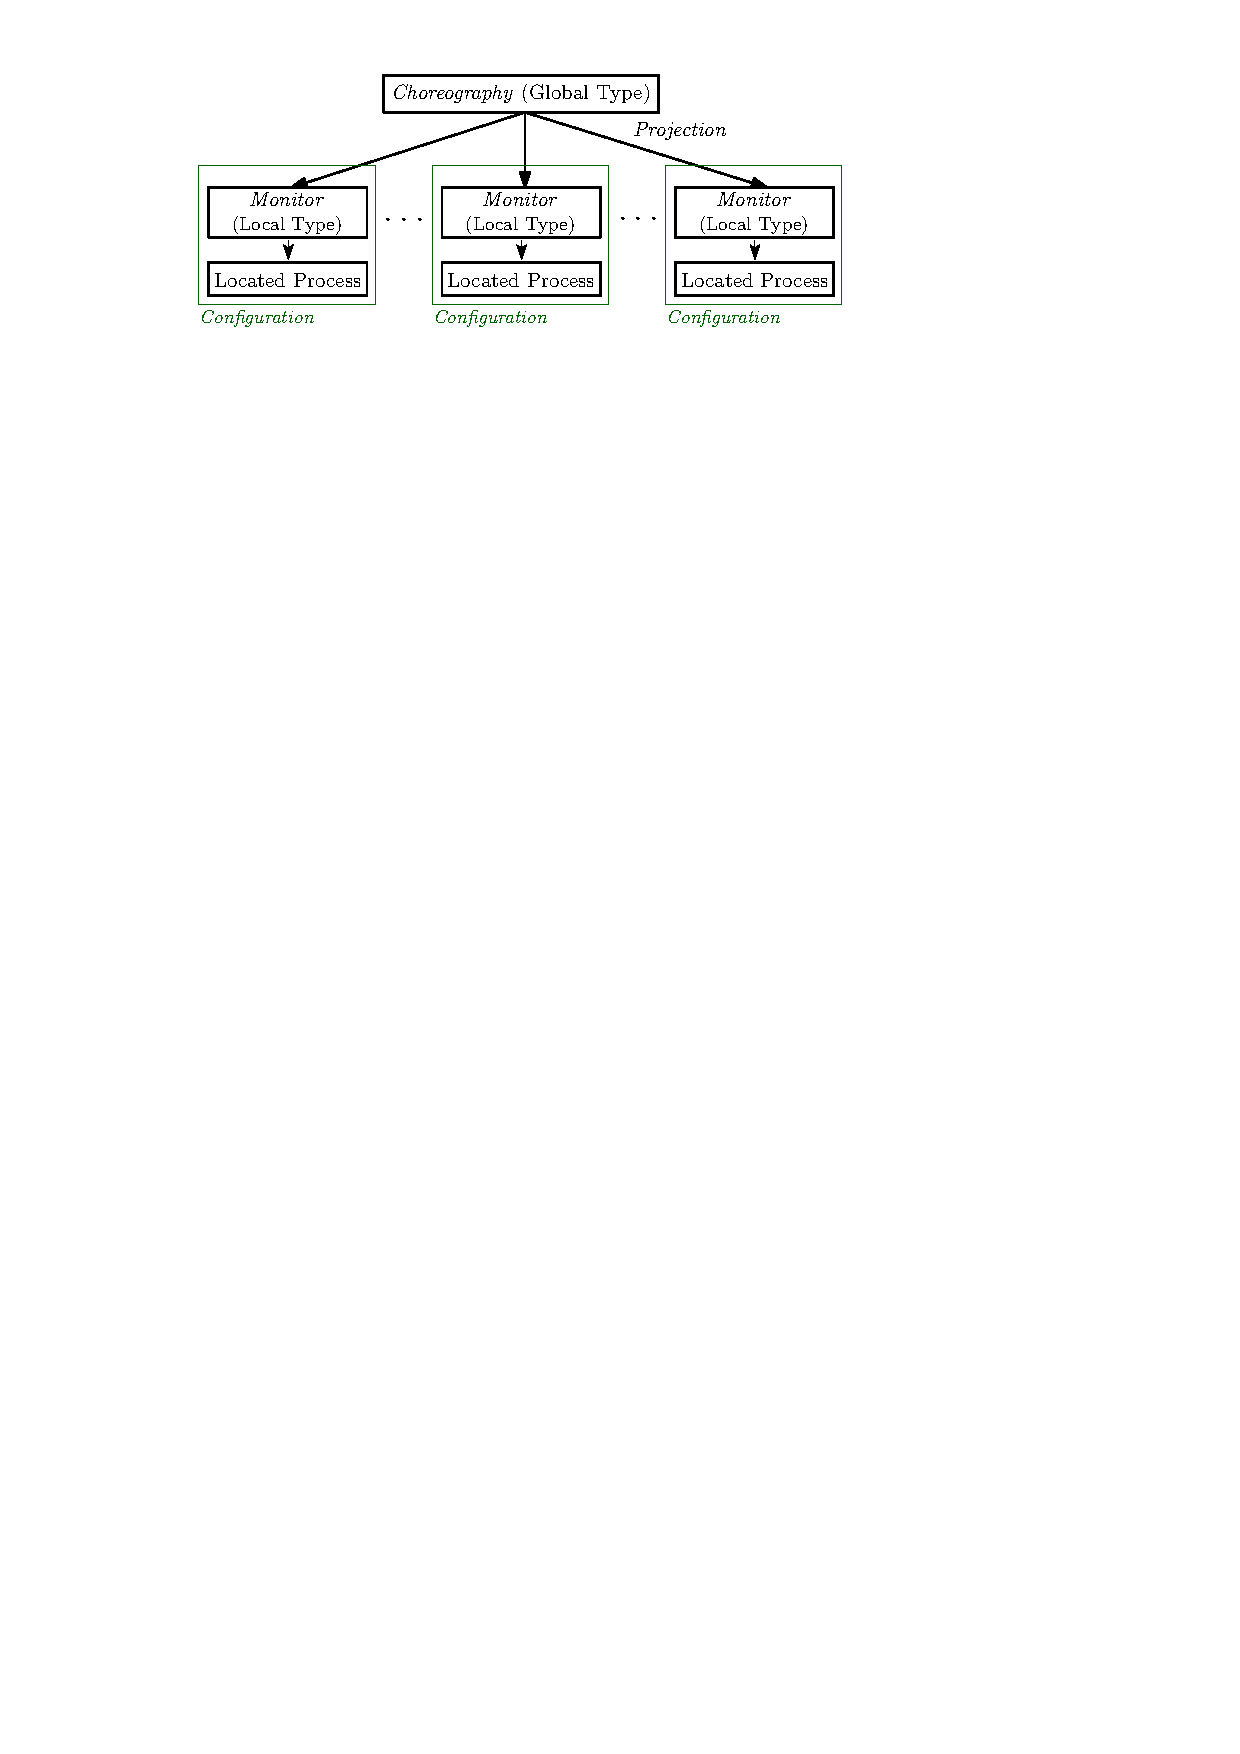
\includegraphics[width=8.7cm]{./img/figmodel.pdf}
\end{center}
\vspace{-4mm}
\caption{The process model of multiparty, reversible communications developed in~\cite{DBLP:conf/ppdp/MezzinaP17}.}\label{f:model}
\end{figure}

Our aim is to develop a Haskell implementation of the process model presented in~\cite{DBLP:conf/ppdp/MezzinaP17}, and depicted in Fig.~\ref{f:model}. 
Here we shall  informally describe the key elements of the model, guided by a running example. Interested readers are referred to~\cite{DBLP:conf/ppdp/MezzinaP17} for further details, in particular the definition and proof of causal consistency. 

\paragraph{Overview.}
Fig.~\ref{f:model} depicts two of the three salient ingredients of the model:
\emph{configurations/processes} and the
\emph{choreography}, which represent the communicating partners and their intended governing protocol, respectively. 
There is a {configuration} for each protocol participant: it includes a \emph{located process} that specifies asynchronous communication behavior and is subject to a \emph{monitor} that enables forward/backward steps at run-time. This monitor is obtained via the choreography, which describes a protocol among two or more \emph{participants}. 
Formally, the model considers choreographies defined in terms of \emph{global types} in the sense of multiparty session types~\cite{DBLP:conf/popl/HondaYC08}. 
(We often use `choreographies' and `global types' as synonyms.)
A global type can be \emph{projected} onto each participant to obtain 
its corresponding  \emph{local type}: a type that abstracts a participant's contribution to the choreography. Since these local types specify the intended sequences of communication actions, they may be used as the monitors of the located processes. 

The third ingredient of the model in~\cite{DBLP:conf/ppdp/MezzinaP17}, not depicted in Fig.~\ref{f:model}, is the operational semantics for configurations. This semantics is defined in terms of two reduction relations, forward and backward, denoted $\fw$  and $\bk$, respectively. We shall not recall these relations here; rather, we will introduce their key underlying intuitions by means of an example.

\paragraph{Syntax of Configurations and Processes.}
The language of processes $P, Q, \ldots$ is a $\pi$-calculus with constructs for labeled (deterministic) choice, communication of abstractions, and function application.
While labeled choice is typical of session $\pi$-calculi (cf.~\cite{DBLP:conf/esop/HondaVK98}), the latter constructs are typical of \emph{higher-order} process calculi, which combine features from functional and concurrent  languages~\cite{DBLP:journals/tcs/Sangiorgi01}. The complete process syntax, with their intuitive semantics, is  as follows:
\begin{align*}
P, Q ::= \, 
        & \bout{u}{V}{P} \,\,\, \, \, &\text{send value $V$ on name $u$, then run $P$} \\
\sbnfbar & \binp{u}{x}{P} \,\,\, \, \, & \text{receive a value on name $u$, bind it to $x$, then run $P$} \\
\sbnfbar &  \bsel{u}{\lbl_i. P_i}_{i\in I}\,\,\, \, \, & \text{select an $l_j$, broadcast this choice, then run $P_j$} \\
\sbnfbar & \bbra{u}{\lbl_i:P_i}_{i \in I} \,\,\, \, \, & \text{receive an   $l_j$, then run  $P_j$} \\
\sbnfbar   & P \Par Q  &\text{parallel composition of $P$ and $Q$} \\
\sbnfbar  & \rvar{X} \sbnfbar  \recp{X}{P} \,\,\, &\text{variable and function abstraction}\\
\sbnfbar & \appl{V}{u} \,\,\, &\text{function application} \\
\sbnfbar  & \news{n}P \,\,\, &\text{name restriction: make $n$ local (or private) to $P$} \\
\sbnfbar  & \inact \,\,\, &\text{terminated process}
\end{align*}
The higher-order character of our process language may be better understood by spelling out the syntax of values $V, W, \ldots$:
\begin{align*}
u,w  \bnfis& n \sbnfbar x,y,z
\qquad \quad
n,n' \bnfis a,b \sbnfbar \ep{s}{\p}
\qquad \quad
 {v},  {v}'  \bnfis   \true \sbnfbar \false \sbnfbar \cdots
\\
V,W \bnfis & {a,b} \sbnfbar  x,y,z \sbnfbar  v, v' \sbnfbar {\abs{x}{P}}
\end{align*}
\noindent 
where  $a,b,c,\ldots$ and $s,s',\ldots$ range over shared and session names, respectively.
Shared names are public names used to establish a protocol (see below); once established, the protocol runs along a session name, which is private to participants.
We   use $\p, \q, \ldots$ to denote  participants, and 
use session names indexed by participants;  we write, e.g., $s_{[\p]}$.
We also use $v,v',\ldots$ to denote
include  (first-order) base values and constants. Variables are denoted  $x,y, \ldots$. 
Values $V$ include shared names, 
first-order values, but also \emph{name abstractions} $\lambda x. P$, where $P$ is a process.
Notice that values need not include (indexed) session names, for session name communication (\emph{delegation}) is  representable using abstraction passing~\cite{KPY2016}.

The syntax of \emph{configurations} $M, N, \ldots$ builds upon that of processes; indeed, we may consider configurations as compositions of located processes:
\begin{align*}
M,N		 \bnfis &
\myloc{\loc}{\bout{a}{x}{P}}
\sbnfbar 
\myloc{\loc}{\binp{a}{x}{P}}
\sbnfbar 
M \Par N 
\sbnfbar 
\news{n} M
\sbnfbar 
\inact 
\\
 \sbnfbar &
{\np{\ep{\loc}{\p}}{\conf{\stack C}{P}}} %% running process
\sbnfbar 
{\monig{\ep{s}{\p}}{H}{\mytilde{x}}{\store}}  %% monitor
\end{align*}
Above,  identifiers $\loc, \loc', \ldots$ denote a  \emph{location} or  \emph{site}. 
The first two constructs enable protocol establishment:
$\myloc{\loc}{\bout{a}{x}{P}}$ is the \emph{request} of a service identified with shared name $a$ implemented by
$P$, whereas $\myloc{\loc}{\binp{a}{x}{P}}$ denotes service \emph{acceptance}. 
Establishing an $n$-party protocol on service $a$ then requires the synchronization of one configuration requesting $a$, and $n-1$ configurations accepting $a$.
Constructs for specifying the composition of configurations, name restriction, and the inactive configuration have expected readings.

The constructs in the second row appear only at run-time (i.e., they do not appear in ``source'' programs) and are key to enable the reversible semantics. We call $\np{\ep{\loc}{\p}}{\conf{\stack C}{P}}$ a \emph{running process}:  $\loc$ hosts a process $P$ that implements participant $\p$, with $\stack C$ being a memory of  labeled choices enforced so far. Configuration $\monig{\ep{s}{\p}}{H}{\mytilde{x}}{\store}$ is a \emph{monitor}
where: 
$s_{[\p]}$ is the indexed session being monitored;
$H$ is a  local type \emph{with history} (see below);
$\mytilde{x}$ is a set of free variables;
and  $\store$ is a store that records the value of such variables.
Moreover, the \emph{tag} $\mytagg$ serves to determine whether 
the running process associated to the monitor is currently involved in a backward step ($\mytagg = \rmark$) or not ($\mytagg = \normark$).

\paragraph{Global and Local Types.}
As already mentioned, choreographies represent multiparty protocols expressed as global types $G, G', \ldots$. Global types can be \emph{projected} onto local types  ($T, T', \ldots$), one per participant. Their syntax follows~\cite{HYC08}:
\begin{align*}
			U, U'  \bnfis & \bool \sbnfbar \nat \sbnfbar \cdots %\bnfbar T 
			\sbnfbar \shot{T} \\
			G, G'  \bnfis & \gtcom{p}{q}{U}{G} %\bnfbar 
			\sbnfbar
			\gtcho{p}{q}{\lbl_i}{G_i} %\\
			\sbnfbar %& 
			\mu X. G \sbnfbar X \sbnfbar \gend \\
	    	T, T'  \bnfis & \ltout{p}{U}{T} \sbnfbar \ltinp{p}{U}{T} %\\
		  \sbnfbar %& 
		  \ltsel{p}{\lbl_i}{T_i}{i}{I} \sbnfbar \ltbra{p}{\lbl_i}{T_i}{i}{I}  
		 %\lsend{p}{\lbl_i}{U_i}{T_i} \bnfbar \lrecv{q}{\lbl_i}{U_i}{T_i} \bnfbar 
		\sbnfbar  \mu X. T \sbnfbar X \sbnfbar \lend 
\end{align*}
\noindent
We briefly discuss value, global, and local types. 
Value types $U$ include basic first-order values,   but also 
the functional type $\shot{T}$ for {higher-order} values: abstractions from names to processes. 
(We write $\Proc$ to denote the type of processes.)

Global type $\gtcom{p}{q}{U}{G}$ says that \p may send a value of type $U$ to \q, and then continue as $G$.
Given a finite index set $I$ and pairwise different {labels} $\lbl_i$, global type $\gtcho{p}{q}{\lbl_i}{G_i}$ specifies that  \p may choose  label $\lbl_i$, send this selection to \q, and then continue as $G_i$.
In these types %thus denote direct communications; 
we assume that $\p \neq \q$.
Recursive and terminated protocols are denoted $\mu X. G$ and $\gend$, respectively.
%We write $\parties{G}$ to denote the set of participants in $G$.

Local types are used in the monitors introduced above. 
Local types
%abstract the behavior of individual participants. Types 
$\ltout{p}{U}{T}$ and $\ltinp{p}{U}{T}$ denote, respectively, an output and input of value of type $U$ by \p.
%\added{We use  $\alpha$ to denote type prefixes  $\typeIn{\p}{U}$, $\typeOut{\p}{U}$.}
Type $\ltbra{p}{\lbl_i}{T_i}{i}{I}$ says that \p 
offers different labeled alternatives;
conversely, type $\ltsel{\p}{\lbl_i}{T_i}{i}{I}$ 
says that \p may select one of such alternatives.
Recursive and terminated local types are denoted $\mu X. T$ and $\lend$, respectively. 
 
 A novelty in~\cite{DBLP:conf/ppdp/MezzinaP17} are \emph{local types with history}  $H, H', \ldots$. Intuitively, a type $H$ is a local type equipped with a
 cursor (denoted $\past$) that serves to distinguish  the (local) protocol actions  that have been already executed (the past of the protocol) from those that are yet to be performed (the future of the protocol).
 
 \paragraph{Projection.}
 Given these intuitions, the projection of a global type $G$ onto a protocol participant $\p$, denoted $\tproj{G}{\gpart{p}}$,  is mostly straightforward, except for choice. 
 The   definition is given in Fig.~\ref{f:proj}.
 Because of recursion, a branch of a choice may recurse back to the beginning.
When this occurs, all participants have to jump back to the beginning,
so every choice must be communicated to all participants.

To deal with this issue, the choice made in~\cite{DBLP:conf/ppdp/MezzinaP17} (as in many other papers) is to disallow different branches using different participants. In practice, 
this means that all branches must perform the same communication to satisfy the global type, even if the communication is not needed in every branch (some branches may have dummy communications). As we will see, in our Haskell implementation we use a different method where every
choice causes a broadcast of that choice to the other participants. 

\begin{figure}[!t]
{
\begin{align*}
\tproj{(\gtcom{p}{q}{U}{G})}{\gpart{r}} & = 
\begin{cases}
\ltout{q}{U}{(\tproj{G}{\gpart{r}})} & \text{if $\gpart{r} = \gpart{p}$} \\
\ltinp{p}{U}{(\tproj{G}{\gpart{r}})} & \text{if $\gpart{r} = \gpart{q}$} \\
(\tproj{G}{\gpart{r}}) &  \text{if $\gpart{r} \neq \gpart{q}, \gpart{r} \neq \gpart{p}$}
\end{cases}
\\
\tproj{(\gtcho{p}{q}{l_i}{G_i})}{\gpart{r}}  
& 
{= 
\begin{cases}
\ltsel{q}{\lbl_i}{(\tproj{G_i}{\gpart{r}})}{i}{I}  & \text{ if $\gpart{r} = \gpart{p}$} \\
\ltbra{p}{\lbl_i}{\tproj{G_i}{\gpart{r}}}{i}{I}  & \text{ if $\gpart{r} = \gpart{q}$} \\
(\tproj{{G_1}}{\gpart{r}}) &  \text{ if $\gpart{r} \neq \gpart{q}, \gpart{r} \neq \gpart{p}$ and} \\ 
& \text{~~$\forall i, j \in I. \tproj{{G_i}}{\gpart{r}} = \tproj{{G_j}}{\gpart{r}}$}
\end{cases}
}
\\
\tproj{(\mu X. G)}{\gpart{r}} &= 
\begin{cases}
\mu X. \tproj{G}{\gpart{r}} & \text{if $\gpart{r}$ occurs in $G$}
\\
\lend & \text{otherwise}
\end{cases}
\\
\tproj{X}{\gpart{r}} & = X
\qquad
\tproj{\gend}{\gpart{r}} = \lend
\end{align*}
}
\vspace{-4mm}
\caption{Projection of a global type $G$ onto a participant $\gpart{r}$~\cite{DBLP:conf/ppdp/MezzinaP17}.\label{f:proj}}
\end{figure}

\paragraph{Example: Three-Buyer Protocol.}
We illustrate the 
forward and backward reduction semantics, denoted \fw and \bk, by example: we recall the running example introduced in~\cite{DBLP:conf/ppdp/MezzinaP17}, namely
  a reversible variant of the \emph{Three-Buyer protocol}  (cf, e.g.,~\cite{CDYP2015})
with abstraction passing. 
The protocol 
involves three buyers (Alice ($\pA$), Bob ($\pB$), Carol ($\pC$)) who interact with a Vendor ($\pS$) as follows:

\begin{enumerate}[1.]
\item Alice sends a book title to Vendor, which replies back to Alice and Bob with a quote. Alice tells Bob how much she can contribute.
\item Bob notifies Vendor and Alice that he agrees with the price, and asks Carol to assist him in completing the protocol. 
To delegate his remaining interactions with Alice and Vendor to Carol, Bob sends her %both an endpoint and 
the code she must execute.
\item Carol continues the rest of the protocol with Vendor and Alice as if she were Bob. 
She sends Bob's address (contained in the  code she received) to Vendor.
\item Vendor answers to Alice and Carol (who represents Bob) with the delivery date.
\end{enumerate}
This protocol may be formalized as the following global type $G$:
\begin{align*}
G = ~&  \gtcom{A}{\pS}{\mathsf{title}}{\gtcom{\pS}{\{A,B\}}{\mathsf{price}}{\gtcom{A}{B}{\mathsf{share}}{
\\
& \quad \gtcom{B}{\{A,\pS\}}{\mathsf{OK}}{
\\
& \quad \gtcom{B}{C}{\mathsf{share}}{\gtcom{B}{C}{\thunkt}{
\\
& \quad \gtcom{B}{\pS}{\mathsf{address}}{\gtcom{\pS}{B}{\mathsf{date}}{\gend}}}}}}}}
%\\
%G_2 = ~& \gtcom{B}{C}{\mathsf{share}}{\gtcom{B}{C}{T}{\gtcom{B}{C}{\shot{T}}{\gend}}}
\end{align*}
Above, we   write
$\gtcom{\p}{\{\q_1,\q_2\}}{U}{G}$
as a shorthand notation for 
$\gtcom{\p}{\q_1}{U}{\gtcom{\p}{\q_2}{U}{G}}$
(and similarly for local types).
Also, we write $\thunkt$ to denote the type $\shot{\lend}$, associated to a \emph{thunk process} $\abs{x}{P}$ with $x \not \in \fn{P}$, written
$\thunkp{P}$. A thunk is an inactive process; it can be activated by applying to it a dummy name of type $\lend$, denoted $\dummyn$.
Moreover, $\mathsf{price}$ and $\mathsf{share}$ are base types treated as integers,
and $\mathsf{title}$, $\mathsf{OK}$, $\mathsf{address}$, and $\mathsf{date}$ are base types treated as strings.
Then we have the following projections of $G$ onto local types:
\begin{align*}
\tproj{G}{\pS} & = \ltinp{A}{\mathsf{title}}{\ltout{\{A,B\}}{\mathsf{price}}{\ltinp{B}{\mathsf{OK}}{\ltinp{B}{\mathsf{address}}{\ltout{B}{\mathsf{date}}{\lend}}}}}
\\
\tproj{G}{\pA} & = \ltout{\pS}{\mathsf{title}}{\ltinp{\pS}{\mathsf{price}}{\ltout{B}{\mathsf{share}}{\ltinp{B}{\mathsf{OK}}{\lend}}}}
\\
\tproj{G}{\pB} & = \ltinp{\pS}{\mathsf{price}}{\ltinp{A}{\mathsf{share}}{\ltout{\{A,\pS\}}{\mathsf{OK}}{
\ltout{C}{\mathsf{share}}{\ltout{C}{\thunkt}{
\\
& \qquad \ltout{\pS}{\mathsf{address}}{\ltinp{\pS}{\mathsf{date}}{\lend}}}}}}}
\\
\tproj{G}{\pC} & = \ltinp{B}{\mathsf{share}}{\ltinp{B}{\thunkt}{\lend}}
\end{align*}
We now give processes for each participant:
\begin{align*}
\text{Vendor} & =  \bout{d}{x:\tproj{G}{\pS}}\binp{x}{t}\bout{x}{price(t)}\bout{x}{price(t)} \binp{x}{ok}\binp{x}{a} \bout{x}{date}\inact  
\\
\text{Alice} & =  \binp{d}{y:\tproj{G}{\pA}}\bout{y}{\exBook}\binp{y}{p}\bout{y}{h}\binp{y}{ok}\inact  
\\
\text{Bob} & =  \binp{d}{z:\tproj{G}{\pB}}\binp{z}{p}\binp{z}{h}\bout{z}{ok}\bout{z}{ok}\bout{z}{h}
  \\
  & \qquad \qquad \bbout{z}{\thunkp{\bout{z}{\text{`Lucca, 55100'}}\binp{z}{d}\inact}}\inact
  \\
\text{Carol} & =  \binp{d}{w:\tproj{G}{\pC}}\binp{w}{h}\binp{w}{code}(\appl{code}{\dummyn})
%&Q_B = \bout{y}{share}\bout{y}{T}\bout{y}{R}\inact  \\
%&Q_C = \binp{y}{share}\binp{y}{T}\binp{y}{X}\inact  \\
\end{align*}
where $price(\cdot)$ returns a value of type $\mathsf{price}$ given a $\mathsf{title}$.
Observe how Bob's implementation sends part of its protocol to Carol as a thunk containing 
his session name and address. 
The whole system, given by configuration $M$ below, is obtained by placing these processes   in appropriate locations ($\loc_1, \ldots, \loc_4$):
$$
M = \myloc{\loc_1}{\text{Vendor}} 
\Par
\myloc{\loc_2}{\text{Alice}} 
\Par
\myloc{\loc_3}{\text{Bob}} 
\Par 
\myloc{\loc_4}{\text{Carol}} 
$$
%\end{document}
We now use $M$ to informally discuss forward and backward reduction rules for \fw and \bk; their formal definition is in~\cite{DBLP:conf/ppdp/MezzinaP17}.
From $M$, the session starts with an application of 
Rule \fwcolor{\textsc{(Init)}}, which initializes the protocol by creating the necessary run-time structures (running processes and monitors):
%To simplify readability, below
%we write 
%$\mathtt{r}$,
%$\mathtt{a}$,
%$\mathtt{b}$,
%and 
%$\mathtt{c}$ 
%instead of participant identities $\mathsf{S}$, $\mathsf{A}$, $\mathsf{B}$, and $\mathsf{C}$, respectively:
%$$
\begin{align*}
%\begin{array}{cc}
M & \fw  \news{s}\big(\, 
\np{\key{{\loc_1}}{\pS}}{ \conf{\inact}{V_1\subst{\epS}{x}}} \Par 
\hmoni{\ep{s}{\pS}}{\past \tproj{G}{\pS}}{x}{\upd{x}{d}}  
\\
& \Par \np{\key{{\loc_2}}{\pA}}{ \conf{\inact}{A_1\subst{\epA}{y}}} \Par 
\hmoni{\ep{s}{\pA}}{\past \tproj{G}{\pA}}{y}{\upd{y}{d}} 
\\
& \Par \np{\key{{\loc_3}}{\pB}}{ \conf{\inact}{B_1\subst{\epB}{z}}} \Par 
\hmoni{\ep{s}{\pB}}{\past \tproj{G}{\pB}}{z}{\upd{z}{d}} 
\\
& \Par \np{\key{{\loc_4}}{\pC}}{ \conf{\inact}{C_1\subst{\epC}{w}}} \Par 
\hmoni{\ep{s}{\pC}}{\past \tproj{G}{\pC}}{w}{\upd{w}{d}}  
  \Par \codah{s}{\emp}{\emp}{}~\big)  = M_1
%\end{array}
\end{align*}
%$$
where 
$V_1$, $A_1$, $B_1$, and $C_1$ 
stand for the continuation of processes $\text{Vendor}$, $\text{Alice}$, $\text{Bob}$, and $\text{Carol}$ after the service 
request/accept. So we have, for instance, 
$
A_1 = \bout{y}{\exBook}\binp{y}{p}\bout{y}{h}\binp{y}{ok}\inact
$.
%Notice also how session initialization instantiates variable ${z}$ in the thunk contained in Bob's implementation with endpoint $\epB$.

From $M_1$ we could either undo the previous reduction (using Rule~\bkcolor{\textsc{(RInit)}})
or execute the communication from $\text{Alice}$ to $\text{Vendor}$ (using two rules:~\fwcolor{\textsc{(Out)}} and ~\fwcolor{\textsc{(In)}}). This latter option would be as follows:
\begin{align*}
M_1 & \fw  \news{s}(\,  \np{\key{{\loc_2}}{\pA}}{ \conf{\inact}{\binp{\epA}{p}\bout{\epA}{h}\binp{\epA}{ok}\inact}} 
\\
& \!\!\!\!\Par 
\hmoni{\ep{s}{\pA}}{\ltout{\pS}{\mathsf{title}}{\past \ltinp{\pS}{\mathsf{price}}{\ltout{B}{\mathsf{share}}{\ltinp{B}{\mathsf{OK}}{\lend}}}}}{y}{\upd{y}{d}} 
\\
& \!\!\!\!\Par N_2 \Par \codah{s}{\emp}{\valueq{\pA}{\pS}{\exBook}}{}~)  = M_2
\end{align*}
where $N_2$ stands for the running processes and monitors for Vendor, Bob, and Carol, who not involved in the reduction.
We now have:
\begin{align*}
M_2 \fw & \news{s}(\,  \np{\key{{\loc_1}}{\pS}}{ \conf{\inact}{\bout{\epS}{price(t)} \bout{\epS}{price(t)}\binp{\epS}{ok}  \binp{\epS}{a} \bout{\epS}{date}\inact }} 
\\
& \Par 
\hmoni{\ep{s}{\pS}}{\ltinp{A}{\mathsf{title}}{\past \ltout{\{A,B\}}{\mathsf{price}}{T_\pS}}}{x,t}{\store_3}  \Par N_3
\\
&  \Par \codah{s}{\valueq{\pA}{\pS}{\exBook}}{\emp}{}~)  = M_3
\end{align*}
where 
$\store_3  = \upd{x}{d},\upd{t}{\exBook}$,
$T_\mathsf{\pS}  = \ltinp{B}{\mathsf{OK}}{\ltinp{B}{\mathsf{address}}{\ltout{B}{\mathsf{date}}{\lend}}}$,
and $N_3$ stands for the participants not involved in the reduction.
Observe that the cursors in monitors $\ep{s}{\pS}$ and $\ep{s}{\pA}$ have evolved, and that the message from $\pA$ to $\pS$ has now been moved to the input queue.

We illustrate  reversibility by showing how to return to $M_1$ from $M_3$.
We need  three backward reduction rules: \bkcolor{\textsc{(RollS)}}, \bkcolor{\textsc{(RIn)}}, and \bkcolor{\textsc{(ROut)}}.
First, Rule~\bkcolor{\textsc{(RollS)}} modifies the tags of monitors $\ep{s}{\pS}$ and $\ep{s}{\pA}$,
  leaving the rest unchanged:
\begin{align*}
M_3 & \bk  \news{s}(\,  
\np{\key{{\loc_1}}{\pS}}{ \conf{\inact}{\bout{\epS}{price(t)}\bout{\epS}{price(t)}\binp{\epS}{ok}  \binp{\epS}{a} \bout{\epS}{date}\inact }} 
\\
& \Par 
 \monir{\ep{s}{\pS}}{\ltinp{A}{\mathsf{title}}{\past \ltout{\{A,B\}}{\mathsf{price}}{T_\mathsf{B}}}}{x,t}{\store_3} 
\\
& \Par \np{\key{{\loc_2}}{\pA}}{ \conf{\inact}{\binp{\epA}{p}\bout{\epA}{h}\binp{\epA}{ok}\inact}} 
\\
& \Par 
\monir{\ep{s}{\pA}}{\myctxr{\ctx{T}_4}{\past \ltinp{\pS}{\mathsf{price}}{\ltout{B}{\mathsf{share}}{\ltinp{B}{\mathsf{OK}}{\lend}}}}}{y}{\upd{y}{d}} 
\\
& \Par N_4 \Par \codah{s}{\valueq{\pA}{\pS}{\exBook}}{\emp}{}~)  = M_4
\end{align*}
where
$\myctxr{\ctx{T}_4}{\bullet}  =\ltout{\pS}{\mathsf{title}}{\bullet}$ and, as before, $N_4$ represents participants not involved in the reduction.
$M_4$ has several possible forward and backward reductions. 
One particular reduction uses Rule~\bkcolor{\textsc{(RIn)}}
to undo the input at \pS:
\begin{align*}
M_4 & \bk  \news{s}(\,  
\np{\key{{\loc_1}}{\pS}}{ \conf{\inact}{\binp{\epS}{t}\bout{\epS}{price(t)}\bout{\epS}{price(t)}   \binp{\epS}{ok}\binp{\epS}{a} \bout{\epS}{date}\inact }} 
\\
& \Par 
 \hmoni{\ep{s}{\pS}}{\past \ltinp{A}{\mathsf{title}}{\ltout{\{A,B\}}{\mathsf{price}}{T_\mathsf{B}}}}{x}{\upd{x}{d}} 
\\
& \Par \np{\key{{\loc_2}}{\pA}}{ \conf{\inact}{\binp{\epA}{p}\bout{\epA}{h}\binp{\epA}{ok}\inact}} 
\\
& \Par 
\monir{\ep{s}{\pA}}{\myctxr{\ctx{T}_4}{\past \ltinp{\pS}{\mathsf{price}}{\ltout{B}{\mathsf{share}}{\ltinp{B}{\mathsf{OK}}{\lend}}}}}{y}{\upd{y}{d}} 
\\
& \Par N_4 \Par \codah{s}{\emp}{\valueq{\pA}{\pS}{\exBook}}{}~)  = M_5
\end{align*}
The following (backward) reduction from $M_5$ undoes the output at \pA:
\begin{align*}
M_5 & \bk  \news{s}(\,  
\np{\key{{\loc_1}}{\pS}}{ \conf{\inact}{\binp{\epS}{t}\bout{\epS}{price(t)}\bout{\epS}{price(t)} \\ 
&   \binp{\epS}{ok}\binp{\epS}{a} \bout{\epS}{date}\inact }} 
\\
&  \!\!\!\! \Par 
 \hmoni{\ep{s}{\pS}}{\!\!\past \ltinp{A}{\mathsf{title}}{\ltout{\{A,B\}}{\mathsf{price}}{T_\mathsf{B}}}}{x}{\upd{x}{d}} 
\\
& \!\!\!\! \Par \np{\key{{\loc_2}}{\pA}}{ \conf{\inact}{\bout{\epA}{\exBook}\binp{\epA}{p}\bout{\epA}{h}\binp{\epA}{ok}\inact}} 
\\
& \!\!\!\!\Par 
\hmoni{\ep{s}{\pA}}{\!\!\past \ltout{\pS}{\mathsf{title}}{\ltinp{\pS}{\mathsf{price}}{\ltout{B}{\mathsf{share}}{\ltinp{B}{\mathsf{OK}}{\lend}}}}}{y}{\upd{y}{d}} 
\\
& \!\!\!\! \Par N_4 \Par \codah{s}{\emp}{\emp}{}~)  = M_6
\end{align*}
Clearly, $M_6 = M_1$.
Summing up, the synchronization realized by the (forward) reduction sequence
$M_1 \fw M_2 \fw M_3$ can be reversed by the (backward) reduction sequence
$M_3 \bk M_4 \bk M_5 \bk M_6$.

To illustrate abstraction passing, let us assume that 
$M_3$ above follows a sequence of forward reductions
until the configuration:
\begin{align*}
M_7 = ~ &   \news{s}(\,  \np{\key{{\loc_3}}{\pB}}{ \conf{\inact}{\bbout{\epB}{\thunkp{\bout{\epB}{\text{`Lucca, 55100'}}\binp{\epB}{d}\inact}}\inact}} 
\\
& \!\!\!\! \Par \hmoni{\ep{s}{\pB}}{\myctxr{\ctx{T}_7}{\past \ltout{C}{\thunkt}{\ltout{\pS}{\mathsf{address}}{\ltinp{\pS}{\mathsf{date}}{\lend}}}}}{z,p,h}{\store_7} 
\\
& \!\!\!\! \Par \np{\key{{\loc_4}}{\pC}}{ \conf{\inact}{\binp{\epC}{code}(\appl{code}{\dummyn})}} 
\\
&  \!\!\!\! \Par 
\hmoni{\ep{s}{\pC}}{\myctxr{\ctx{T}_8}{\past \ltinp{B}{\thunkt}{\lend}}}{w,h}{\store_8} 
\Par N_5 \Par \codah{s}{h_7}{\emp}{}~) 
\end{align*}
where 
$\myctxr{\ctx{T}_7}{\bullet}$, $\store_7$, $\myctxr{\ctx{T}_8}{\bullet}$, $\store_8$,
and $h_7$ capture past interactions as follows:
\begin{align*}
\myctxr{\ctx{T}_7}{\bullet} & =
\ltinp{\pS}{\mathsf{price}}{\ltinp{A}{\mathsf{share}}{\ltout{\{A,\pS\}}{\mathsf{OK}}{
\ltout{C}{\mathsf{share}}{\bullet}}}}
\\
\store_7 & = \upd{z}{d},\upd{p}{price(\exBook)},\upd{h}{120}
\\
\myctxr{\ctx{T}_8}{\bullet} & =\ltinp{B}{\mathsf{share}}{\bullet} \qquad \store_8  = \upd{w}{d},\upd{h}{120}
\\
h_7 & = 
\valueq{\pA}{\pS}{\exBook}
\\
& \cons
\valueq{\pS}{\pA}{price(\exBook)}
\cons
\valueq{\pS}{\pB}{price(\exBook)}
\\
& \cons
\valueq{\pA}{\pB}{120}
\cons
\valueq{\pB}{\pA}{\text{`ok'}}
\cons
\valueq{\pB}{\pS}{\text{`ok'}}
\cons
\valueq{\pB}{\pC}{120}
\end{align*}
%Also, $120 - price(\exBook)$ is the amount \pB may contribute.

If $M_7 \fw \fw M_8$ by using Rules~\fwcolor{\textsc{(Out)}} and ~\fwcolor{\textsc{(In)}}
we would have:
\begin{align*}
M_8 & = ~   \news{s}(\,  \np{\key{{\loc_3}}{\pB}}{ \conf{\inact}{\inact}} 
\\
& \Par \hmoni{\ep{s}{\pB}}{\myctxr{\ctx{T}_7}{\ltout{C}{\thunkt}{\past\ltout{\pS}{\mathsf{address}}{\ltinp{\pS}{\mathsf{date}}{\lend}}}}}{z,p,h}{\store_7} 
\\
& \Par \np{\key{{\loc_4}}{\pC}}{ \conf{\inact}{(\appl{code}{\dummyn}) }} 
 \Par 
\hmoni{\ep{s}{\pC}}{\myctxr{\ctx{T}_8}{ \ltinp{B}{\thunkt}{\past\lend}}}{w,h,code}{\store_9} 
\\
& 
\Par N_5 \Par \codah{s}{h_7 \cons \valueq{\pB}{\pC}{\thunkp{\bout{\epB}{\text{`Lucca, 55100'}}\binp{\epB}{d}\inact}}}{\emp}{}~) 
\end{align*}
where
$\store_9 = \store_8 \upd{code}{\thunkp{\bout{\epB}{\text{`Lucca, 55100'}}\binp{\epB}{d}\inact}}$.
We now may apply Rule~\fwcolor{\textsc{(Beta)}} to obtain the actual code sent from \pB to \pC:
\begin{align*}
M_8 & \fw ~   \news{s}\news{k}(\,  
%\np{\key{\loc_3}{\pB}}{ \conf{\inact}{\inact}} 
%\\
%& \Par \hmoni{s_\pB}{\myctxr{\ctx{T}_7}{\ltout{C}{\thunkt}{\past\ltout{S}{\mathsf{address}}{\ltinp{S}{\mathsf{date}}{\lend}}}}}{z,p,s}{\store_7} 
%\\
%& \Par 
\np{\key{{\loc_4}}{\pC}}{\conf{\inact}{\bout{\epB}{\text{`Lucca, 55100'}}\binp{\epB}{d}\inact}} 
\!\!  \Par N_6 
\\
& \!\!\Par \hmoni{\ep{s}{\pB}}{\myctxr{\ctx{T}_7}{\ltout{C}{\thunkt}{\past\ltout{\pS}{\mathsf{address}}{\ltinp{\pS}{\mathsf{date}}{\lend}}}}}{z,p,h}{\store_7} 
\\
& \!\!\Par 
\mem{k}{(\appl{code}{\dummyn})}{{\loc_4}} 
\Par 
\hmoni{\ep{s}{\pC}}{\myctxr{\ctx{T}_8}{ \ltinp{B}{\thunkt}{k.\past\lend}}}{w,h,code}{\store_9} 
\\
& 
\!\!\Par \codah{s}{h_7 \cons \valueq{\pB}{\pC}{\thunkp{\bout{\epB}{\text{`Lucca, 55100'}}\binp{\epB}{d}\inact}}}{\emp}{}~) 
= M_9
\end{align*}
where $N_6$ is the rest of the system. 
Notice that this reduction has added a running function on a fresh 
$k$, which is also used within the type stored in the monitor $\ep{s}{\pC}$.

The reduction $M_8 \fw M_9$ completes the code mobility from $\pB$ to $\pC$: the now active thunk
will execute $\pB$'s implementation from $\pC$'s location. Observe that Bob's identity \pB is ``hardwired'' in the sent thunk; 
there is no way for \pC to execute the code by referring to a participant different  from \pB.
%This justifies the premise 
%$\p = \er \,\vee\, \p \in \names{\er, h_i}$ present in Rules~\fwcolor{\textsc{(Out)}} and \fwcolor{\textsc{(In)}} 
%\erase{\fwcolor{\textsc{(Sel)}} and ~\fwcolor{\textsc{(Bra)}}} (and in their backward counterparts):
When executing previously received mobile code, the participant mentioned in the location (i.e., $\pC$)
and that mentioned in the located process (i.e., $\pB$) may differ.
Further forward reductions from $M_9$ will  modify the cursor in the type stored in monitor $\ep{s}{\pB}$
based on the process located at $\key{{\loc_4}}{\pC}$.



\section{IMPLEMENTATION}
\textbf{\emph{In this section we show how we implement the processes, types, and semantics in the PPDP paper}}

\subsection{Implementing the PPDP'17 calculus in
Haskell}\label{implementing-the-ppdp17-calculus-in-haskell}

The implementation uses an algebraic data type (also known as union type or sum type) to
encode all the constructors of $P$, the process syntax. We use the \texttt{Fix} type
(Appendix \ref{fix}) to factor out recursion from the grammar.
\texttt{Fix} is the fixed point type:

\begin{Shaded}
\begin{Highlighting}[]
\KeywordTok{data} \DataTypeTok{Fix}\NormalTok{ f }\FunctionTok{=} \DataTypeTok{Fix}\NormalTok{ (f (}\DataTypeTok{Fix}\NormalTok{ f))}
\end{Highlighting}
\end{Shaded}

\texttt{Fix} allows us to concisely express an infinite nesting of a
type (of the shape \texttt{f\ (f\ (f\ (f\ (..))))}). Such a type will
look like a tree. For the values of this type to be finite, the
\texttt{f} must have a leaf constructor. Take for instance this simple
expression language

\begin{Shaded}
\begin{Highlighting}[]
\KeywordTok{data} \DataTypeTok{Expr}
    \FunctionTok{=} \DataTypeTok{Literal} \DataTypeTok{Int}
    \FunctionTok{|} \DataTypeTok{Add} \DataTypeTok{Expr} \DataTypeTok{Expr} 
\end{Highlighting}
\end{Shaded}

\texttt{Literal} is the only constructor that can occur as a leaf, and
\texttt{Add} is the only node. Using \texttt{Fix} we can equivalently
write

\begin{Shaded}
\begin{Highlighting}[]
\KeywordTok{data} \DataTypeTok{ExprF}\NormalTok{ next}
    \FunctionTok{=} \DataTypeTok{Literal} \DataTypeTok{Int}
    \FunctionTok{|} \DataTypeTok{Add}\NormalTok{ next next }
\end{Highlighting}
\end{Shaded}

In the above snippet, \texttt{next} is a placeholder or hole for an
arbitrarily deep nesting of \texttt{ExprF}s. The main usage of
\texttt{Fix} is that it gives traversals and folds of our syntax tree
for free because these are generically defined on \texttt{Fix}.

\begin{Shaded}
\begin{Highlighting}[]
\OtherTok{simple ::} \DataTypeTok{Fix} \DataTypeTok{ExprF}
\NormalTok{simple }\FunctionTok{=} \DataTypeTok{Fix}\NormalTok{ (}\DataTypeTok{Literal} \DecValTok{42}\NormalTok{)}

\OtherTok{complex ::} \DataTypeTok{Fix} \DataTypeTok{ExprF}
\NormalTok{complex }\FunctionTok{=} 
    \DataTypeTok{Fix}\NormalTok{ (}\DataTypeTok{Add}\NormalTok{ (}\DataTypeTok{Fix}\NormalTok{ (}\DataTypeTok{Literal} \DecValTok{40}\NormalTok{)) (}\DataTypeTok{Fix}\NormalTok{ (}\DataTypeTok{Literal} \DecValTok{2}\NormalTok{)))}
\end{Highlighting}
\end{Shaded}

The above snippet shows that defining values of type \texttt{Fix\ ExprF}
requires wrapping of constructors with \texttt{Fix}. We will describe a
better way of writing \texttt{Fix}ed values in Section
\ref{free-monad-dsl}.

The full definition of \texttt{Program} is given below. As mentioned we
omit the process-level recursion, but otherwise it is a direct translation of the formal syntax given in Section \ref{the-process-model}.

\begin{Shaded}
\begin{Highlighting}[]
\KeywordTok{type} \DataTypeTok{Participant} \FunctionTok{=} \DataTypeTok{String}
\KeywordTok{type} \DataTypeTok{Identifier} \FunctionTok{=} \DataTypeTok{String}

\KeywordTok{type} \DataTypeTok{Program}\NormalTok{ value }\FunctionTok{=} \DataTypeTok{Fix}\NormalTok{ (}\DataTypeTok{ProgramF}\NormalTok{ value) }

\KeywordTok{data} \DataTypeTok{ProgramF}\NormalTok{ value next }
    \CommentTok{-- communication primitives}
    \FunctionTok{=} \DataTypeTok{Send} 
\NormalTok{        \{}\OtherTok{ owner ::} \DataTypeTok{Participant}
\NormalTok{        ,}\OtherTok{ value ::}\NormalTok{ value}
\NormalTok{        ,}\OtherTok{ continuation ::}\NormalTok{ next }
\NormalTok{        \}}
    \FunctionTok{|} \DataTypeTok{Receive} 
\NormalTok{        \{}\OtherTok{ owner ::} \DataTypeTok{Participant}
\NormalTok{        ,}\OtherTok{ variableName ::} \DataTypeTok{Identifier}
\NormalTok{        ,}\OtherTok{ continuation ::}\NormalTok{ next  }
\NormalTok{        \}}

    \CommentTok{-- choice primitives}
    \FunctionTok{|} \DataTypeTok{Offer} \DataTypeTok{Participant}\NormalTok{ (}\DataTypeTok{List}\NormalTok{ (}\DataTypeTok{String}\NormalTok{, next))}
    \FunctionTok{|} \DataTypeTok{Select} \DataTypeTok{Participant}\NormalTok{ (}\DataTypeTok{List}\NormalTok{ (}\DataTypeTok{String}\NormalTok{, value, next))}

    \CommentTok{-- other constructors }
    \FunctionTok{|} \DataTypeTok{Parallel}\NormalTok{ next next }
    \FunctionTok{|} \DataTypeTok{Application} \DataTypeTok{Identifier}\NormalTok{ value}
    \FunctionTok{|} \DataTypeTok{NoOp}
    \KeywordTok{deriving}\NormalTok{ (}\DataTypeTok{Functor}\NormalTok{) }
\end{Highlighting}
\end{Shaded}

We also need values in our language. To write more interesting examples
we extend the types of values that can be used from names, booleans and
functions to also include references, integers, strings, and basic
integer and comparison operators.

\begin{Shaded}
\begin{Highlighting}[]
\KeywordTok{data} \DataTypeTok{Value} 
    \FunctionTok{=} \DataTypeTok{VBool} \DataTypeTok{Bool}
    \FunctionTok{|} \DataTypeTok{VInt} \DataTypeTok{Int}
    \FunctionTok{|} \DataTypeTok{VString} \DataTypeTok{String}
    \FunctionTok{|} \DataTypeTok{VUnit}
    \FunctionTok{|} \DataTypeTok{VIntOperator} \DataTypeTok{Value} \DataTypeTok{IntOperator} \DataTypeTok{Value} 
    \FunctionTok{|} \DataTypeTok{VComparison} \DataTypeTok{Value} \DataTypeTok{Ordering} \DataTypeTok{Value}
    \FunctionTok{|} \DataTypeTok{VFunction} \DataTypeTok{Identifier}\NormalTok{ (}\DataTypeTok{Program} \DataTypeTok{Value}\NormalTok{)}
    \FunctionTok{|} \DataTypeTok{VReference} \DataTypeTok{Identifier} 
    \FunctionTok{|} \DataTypeTok{VLabel} \DataTypeTok{String}
\end{Highlighting}
\end{Shaded}

We can now write processes like the one below. It first sends the value $42$ and then expects to receive a value that it will bind to identifier $y$.

\begin{Shaded}
\begin{Highlighting}[]
\NormalTok{example }\FunctionTok{=} 
    \DataTypeTok{Fix} 
\NormalTok{        ( }\DataTypeTok{Parallel} 
\NormalTok{            (}\DataTypeTok{Fix}\NormalTok{ (}\DataTypeTok{Send} \StringTok{"me"}\NormalTok{ (}\DataTypeTok{VInt} \DecValTok{42}\NormalTok{) (}\DataTypeTok{Fix} \DataTypeTok{NoOp}\NormalTok{)))}
\NormalTok{            (}\DataTypeTok{Fix}\NormalTok{ (}\DataTypeTok{Receive} \StringTok{"you"} \StringTok{"y"}\NormalTok{ (}\DataTypeTok{Fix} \DataTypeTok{NoOp}\NormalTok{)))}
\NormalTok{        )}
\end{Highlighting}
\end{Shaded}

While the above is easily manipulatable with pattern matching and
functions from the \texttt{Fix} module, it is very hard to write clear
examples in this style. Longer expressions need ever more parentheses
and in general there is too much syntactical clutter. We will get back
to designing a better syntax for defining programs in Section
\ref{free-monad-dsl}.

\subsection{Global Types}

Much like the process syntax, the Haskell implementation of global types closely mimics the formal definition.
Its implementation is given by: 

\begin{Shaded}
\begin{Highlighting}[]
\KeywordTok{type} \DataTypeTok{GlobalType}\NormalTok{ participant u }\FunctionTok{=} 
    \DataTypeTok{Free}\NormalTok{ (}\DataTypeTok{GlobalTypeF}\NormalTok{ participant u) }\DataTypeTok{Void}

\KeywordTok{data} \DataTypeTok{GlobalTypeF}\NormalTok{ participant u next}
    \FunctionTok{=} \DataTypeTok{Transaction} 
\NormalTok{        \{}\OtherTok{ from ::}\NormalTok{ participant}
\NormalTok{        ,}\OtherTok{ to ::}\NormalTok{ participant}
\NormalTok{        ,}\OtherTok{ tipe ::}\NormalTok{ u}
\NormalTok{        ,}\OtherTok{ continuation ::}\NormalTok{  next }
\NormalTok{        \} }
    \FunctionTok{|} \DataTypeTok{Choice} 
\NormalTok{        \{}\OtherTok{ from ::}\NormalTok{ participant}
\NormalTok{        ,}\OtherTok{ to ::}\NormalTok{ participant}
\NormalTok{        ,}\OtherTok{ options ::} \DataTypeTok{Map} \DataTypeTok{String}\NormalTok{ next }
\NormalTok{        \}}
    \FunctionTok{|} \DataTypeTok{End}
    \FunctionTok{|} \DataTypeTok{RecursionPoint}\NormalTok{ next}
    \FunctionTok{|} \DataTypeTok{RecursionVariable}
    \FunctionTok{|} \DataTypeTok{Weaken}\NormalTok{ next}
    \KeywordTok{deriving}\NormalTok{ (}\DataTypeTok{Functor}\NormalTok{)}
\end{Highlighting}
\end{Shaded}

We can now see why choice is useful: it allows us to branch on the
session type level. For instance, one branch can terminate the protocol,
and the other can loop back to start the protocol again from the beginning.

The final three constructors are required for supporting nested
recursion and taken from \cite{van2017session}. A
\texttt{RecursionPoint} is a point in the protocol that we can later
jump back to. A \texttt{RecursionVariable} triggers jumping to a
previously encountered \texttt{RecursionPoint}. By default it will jump
to the closest and most-recently encountered \texttt{RecursionPoint},
but \texttt{WeakenRecursion} makes it jump one \texttt{RecursionPoint}
higher, encountering 2 weakens will jump 2 levels higher etc.

Using \texttt{Monad.Free} (Appendix \ref{free-monad}), we can write
examples with a more idiomatic Haskell syntax.

The snippet below shows the use of nested recursion. There is an outer
loop that will perform a piece of protocol or end, and an inner loop
that sends messages from \texttt{A} to \texttt{B}. When the inner loop
is done, control flow returns to the outer loop.

\begin{Shaded}
\begin{Highlighting}[]
\KeywordTok{import }\DataTypeTok{GlobalType} \KeywordTok{as} \DataTypeTok{G}

\NormalTok{G.recurse }\FunctionTok{$} \CommentTok{-- recursion point 1}
\NormalTok{    G.oneOf }\DataTypeTok{A} \DataTypeTok{B}
\NormalTok{        [ (}\StringTok{"loop"}
\NormalTok{          , G.recurse }\FunctionTok{$} \CommentTok{-- recursion point 2}
\NormalTok{                G.oneOf }\DataTypeTok{A} \DataTypeTok{B}
\NormalTok{                    [ (}\StringTok{"continueLoop"}\NormalTok{, }\KeywordTok{do} 
\NormalTok{                        G.message }\DataTypeTok{A} \DataTypeTok{B} \StringTok{"date"}
                        \CommentTok{-- jumps to recursion point 2}
\NormalTok{                        G.recursionVariable}
\NormalTok{                      )}
            
\NormalTok{                    , (}\StringTok{"endInnerLoop"}\NormalTok{, }\KeywordTok{do} 
                        \CommentTok{-- jumps to recursion point 1}
\NormalTok{                        G.weakenRecursion G.recursionVariable}
\NormalTok{                      )}
\NormalTok{                    ]}
\NormalTok{          )}
\NormalTok{        , (}\StringTok{"end"}\NormalTok{, G.end)}
\NormalTok{        ]}
\end{Highlighting}
\end{Shaded}

Similarly, the three buyer example can be written as:

\begin{Shaded}
\begin{Highlighting}[]
\CommentTok{-- a data type representing the participants}
\KeywordTok{data} \DataTypeTok{MyParticipants} \FunctionTok{=} \DataTypeTok{A} \FunctionTok{|} \DataTypeTok{B} \FunctionTok{|} \DataTypeTok{C} \FunctionTok{|} \DataTypeTok{V} 
    \KeywordTok{deriving}\NormalTok{ (}\DataTypeTok{Show}\NormalTok{, }\DataTypeTok{Eq}\NormalTok{, }\DataTypeTok{Ord}\NormalTok{, }\DataTypeTok{Enum}\NormalTok{, }\DataTypeTok{Bounded}\NormalTok{)}

\CommentTok{-- a data type representing the used types }
\KeywordTok{data} \DataTypeTok{MyType} \FunctionTok{=} \DataTypeTok{Title} \FunctionTok{|} \DataTypeTok{Price} \FunctionTok{|} \DataTypeTok{Share} \FunctionTok{|} \DataTypeTok{Ok} \FunctionTok{|} \DataTypeTok{Thunk} \FunctionTok{|} \DataTypeTok{Address} \FunctionTok{|} \DataTypeTok{Date}
    \KeywordTok{deriving}\NormalTok{ (}\DataTypeTok{Show}\NormalTok{, }\DataTypeTok{Eq}\NormalTok{, }\DataTypeTok{Ord}\NormalTok{)}

\CommentTok{-- a description of the protocol}
\OtherTok{globalType ::} \DataTypeTok{GlobalType.GlobalType} \DataTypeTok{MyParticipants} \DataTypeTok{MyType}
\NormalTok{globalType }\FunctionTok{=} \KeywordTok{do} 
\NormalTok{    message }\DataTypeTok{A} \DataTypeTok{V} \DataTypeTok{Title} 
\NormalTok{    messages }\DataTypeTok{V}\NormalTok{ [}\DataTypeTok{A}\NormalTok{, }\DataTypeTok{B}\NormalTok{] }\DataTypeTok{Price} 
\NormalTok{    message }\DataTypeTok{A} \DataTypeTok{B} \DataTypeTok{Share} 
\NormalTok{    messages }\DataTypeTok{B}\NormalTok{ [}\DataTypeTok{A}\NormalTok{, }\DataTypeTok{V}\NormalTok{] }\DataTypeTok{Ok} 
\NormalTok{    message }\DataTypeTok{B} \DataTypeTok{C} \DataTypeTok{Share}
\NormalTok{    message }\DataTypeTok{B} \DataTypeTok{C} \DataTypeTok{Thunk}
\NormalTok{    message }\DataTypeTok{B} \DataTypeTok{V} \DataTypeTok{Address}
\NormalTok{    message }\DataTypeTok{V} \DataTypeTok{B} \DataTypeTok{Date}
\NormalTok{    end}
\end{Highlighting}
\end{Shaded}

\subsection{A Reversible Semantics}\label{a-reversible-semantics}

The third component of the system a reversible semantics. The idea here
is that we can move back to previous program states, reversing forward
steps.

To be able to move backward, we need to store some information when we move forward.
The PPDP'17 paper tells us that, broadly, we need to track information about two things: the type and the
process.

For the type we define a new data type called \texttt{TypeContext}. It
contains the actions that have been performed and for some of them it
stores a bit of extra information like the \texttt{owner}.

On the process level there are four things that we need to track:

\begin{enumerate}
\def\labelenumi{\arabic{enumi}.}
\item
  Used variable names in receives

  The rest of the program depends on the name that is assigned to a
  received value, like \texttt{decision} in the example below.\\
  When reverting, we need to reinstate the name that the rest of the
  program expects.

\begin{Shaded}
\begin{Highlighting}[]
\NormalTok{decision }\OtherTok{<-}\NormalTok{ H.receive    }
\NormalTok{H.send decision          }
\end{Highlighting}
\end{Shaded}

  When we advance the snippet above, \texttt{decision} is internally
  renamed to \texttt{var1} and this binding is added to the store.

\begin{Shaded}
\begin{Highlighting}[]
\NormalTok{H.send var1        }
\end{Highlighting}
\end{Shaded}

  Now we want to move back. We can't simply create a new name: if we
  then move forward again, \texttt{var1} will not be defined.

\begin{Shaded}
\begin{Highlighting}[]
\NormalTok{var2 }\OtherTok{<-}\NormalTok{ H.receive       }
\NormalTok{H.send var1             }
\end{Highlighting}
\end{Shaded}

  Instead, the receive needs to store the name of the value its result
  is bound to, in this case \texttt{var1}:

\begin{Shaded}
\begin{Highlighting}[]
\NormalTok{var1 }\OtherTok{<-}\NormalTok{ H.receive}
\NormalTok{H.send var1}
\end{Highlighting}
\end{Shaded}

  But we also store the original name (given by the programmer) and
  actually restore that. The original name can helpful in debugging
  programs, to know what value is actually used:

\begin{Shaded}
\begin{Highlighting}[]
\NormalTok{decision }\OtherTok{<-}\NormalTok{ H.receive}
\NormalTok{H.send decision}
\end{Highlighting}
\end{Shaded}
\item
  Unused branches

  When a choice is made and then reverted, we want all our options to be
  available again. Currently, another label cannot actually be selected
  after reverting: the selected label depends only on the values of
  variables in the program. Future work may make it possible to also use
  the failure information to influence the choice made.

\begin{Shaded}
\begin{Highlighting}[]
\KeywordTok{type} \DataTypeTok{Zipper}\NormalTok{ a }\FunctionTok{=}\NormalTok{ (}\DataTypeTok{List}\NormalTok{ a, a, }\DataTypeTok{List}\NormalTok{ a)}

\KeywordTok{data} \DataTypeTok{OtherOptions}
    \FunctionTok{=} \DataTypeTok{OtherSelections}\NormalTok{ (}\DataTypeTok{Zipper}\NormalTok{ (}\DataTypeTok{String}\NormalTok{, }\DataTypeTok{Value}\NormalTok{, }\DataTypeTok{Program} \DataTypeTok{Value}\NormalTok{))}
    \FunctionTok{|} \DataTypeTok{OtherOffers}\NormalTok{ (}\DataTypeTok{Zipper}\NormalTok{ (}\DataTypeTok{String}\NormalTok{, }\DataTypeTok{Program} \DataTypeTok{Value}\NormalTok{))}
\end{Highlighting}
\end{Shaded}

  The code above shows how the choices are stored. We need to remember
  which choice was made, and the order of the options is important. We
  use a \texttt{Zipper} to store the elements in order and use the
  central \texttt{a} to store the choice that was made.
\item
  Function applications

  When applying a function we lose information about the applied
  function and the argument. Therefore we store them in a map and
  associate them with a unique identifier. This identifier is given to
  the \texttt{Application} constructor so when stepping backward the
  function and the argument can be recovered.

  You might think that a stack would be a simpler solution, but a stack
  can give invalid behavior. Say that a participant is running in two
  locations, and the last-performed action at both locations is a
  function application. Now we want to undo both applications, but the
  order in which to undo them is undefined: we need both orders to work.
  When the application keeps track of exactly which function and
  argument it used the end result is always the same. Only using a stack
  could mix up the applications.
\item
  Messages on the channel

  When a value is sent, the sender loses track of what has been sent.
  Therefore, reverting a send/receive pair must move the value from the
  receiver via the queue back to the sender. Fig.
  \ref{fig:reverse-send-receive} below illustrates this process:

  \begin{figure}[h!]
  \begin{align*}
  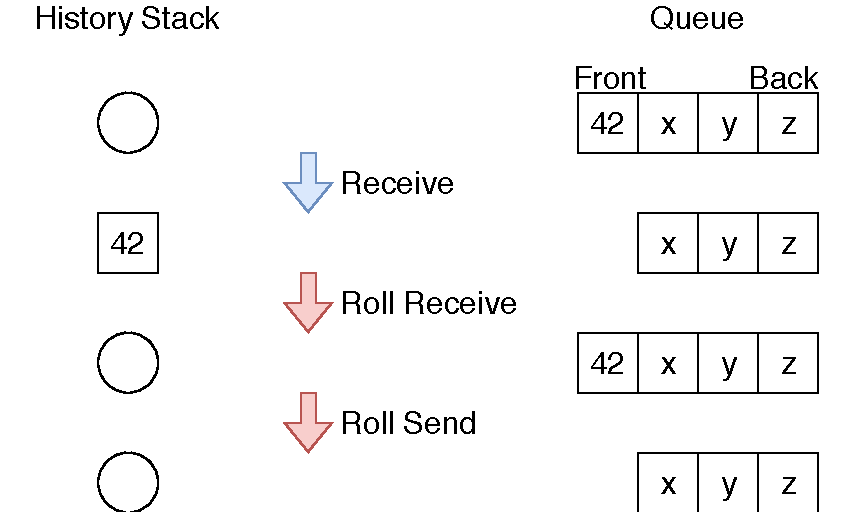
\includegraphics[scale=0.60]{img/queue-history-stack.pdf}
  \end{align*}
  \caption{Reversal of send and receive}
  \label{fig:reverse-send-receive}
  \end{figure}

  \begin{enumerate}
  \def\labelenumii{\arabic{enumii}.}
  \tightlist
  \item
    \textbf{receive}: the value 42 is popped from the queue but pushed
    onto the history stack.
  \item
    \textbf{roll receive}: Now when the receive is rolled, the value is
    moved back from the history stack onto the queue.
  \item
    \textbf{roll send}: When the send is rolled the value is moved from
    the head of the queue into the sender's process.
  \end{enumerate}
\end{enumerate}

\subsection{Abstraction Passing is Protocol
Delegation}\label{abstraction-passing}

Protocol delegation is where a participant can delegate (a part of)
their protocol to be fulfilled by another participant. An example of
where this idea is useful is a load balancing server: from the client's
perspective, the server handles the request, but actually the load
balancer delegates incoming requests to workers. The client does not
need to be aware of this implementation detail.

Recall the definition of \texttt{ProgramF}:

\begin{Shaded}
\begin{Highlighting}[]
\KeywordTok{data} \DataTypeTok{ProgramF}\NormalTok{ value next }
    \CommentTok{-- communication primitives}
    \FunctionTok{=} \DataTypeTok{Send} 
\NormalTok{        \{}\OtherTok{ owner ::} \DataTypeTok{Participant}
\NormalTok{        ,}\OtherTok{ value ::}\NormalTok{ value}
\NormalTok{        ,}\OtherTok{ continuation ::}\NormalTok{ next }
\NormalTok{        \}}
    \FunctionTok{|} \FunctionTok{...} 
\end{Highlighting}
\end{Shaded}

The \texttt{ProgramF} constructors that move the local type forward
(send/receive, select/offer) have an \texttt{owner} field that stores
whose local type they should be checked agains and modfiy. This field is
also present in the \texttt{TypeContext}.

Because we allow references to values in the implementation, all
references in a function have to be dereferenced before it can be safely
sent over a channel.


\subsection{Putting it all together}\label{combining}

With all the definitions encoded, we can now define forward and backward
evaluation of our system. Our aim is to implement:

\begin{Shaded}
\begin{Highlighting}[]
\OtherTok{forward  ::} \DataTypeTok{Location} \OtherTok{->} \DataTypeTok{Session}\NormalTok{ ()}
\OtherTok{backward ::} \DataTypeTok{Location} \OtherTok{->} \DataTypeTok{Session}\NormalTok{ ()}
\end{Highlighting}
\end{Shaded}

These functions take a \texttt{Location}, our way of modeling different
threads or machines, and tries to move the process at that location
forward or backward. The \texttt{Session} type contains the
\texttt{ExecutionState}, the state of the session (all programs, local
types, variable bindings, etc.), and can throw errors of type
\texttt{Error}, for instance when an unbound variable is used.

\begin{Shaded}
\begin{Highlighting}[]
\KeywordTok{type} \DataTypeTok{Session}\NormalTok{ a }\FunctionTok{=} \DataTypeTok{StateT} \DataTypeTok{ExecutionState}\NormalTok{ (}\DataTypeTok{Except} \DataTypeTok{Error}\NormalTok{) a}
\end{Highlighting}
\end{Shaded}

\emph{See also Appendices \ref{state} on \texttt{StateT} and
\ref{except} on \texttt{Except}}

The semantics in the PPDP'17 paper guides how we store the execution
state. Some data is bound to its location (for instance the process that
is running) and other data is bound to its participant (for instance the
local type).

The information about a participant grouped in a type called
\texttt{Monitor}:

\begin{Shaded}
\begin{Highlighting}[]
\KeywordTok{data} \DataTypeTok{Monitor}\NormalTok{ value tipe }\FunctionTok{=} 
    \DataTypeTok{Monitor} 
\NormalTok{        \{}\OtherTok{ _localType ::} \DataTypeTok{LocalTypeState}\NormalTok{ tipe}
\NormalTok{        ,}\OtherTok{ _recursiveVariableNumber ::} \DataTypeTok{Int}
\NormalTok{        ,}\OtherTok{ _recursionPoints ::} \DataTypeTok{List}\NormalTok{ (}\DataTypeTok{LocalType}\NormalTok{ tipe)}
\NormalTok{        ,}\OtherTok{ _usedVariables ::} \DataTypeTok{List} \DataTypeTok{Binding} 
\NormalTok{        ,}\OtherTok{ _applicationHistory ::} \DataTypeTok{Map} \DataTypeTok{Identifier}\NormalTok{ (value, value)}
\NormalTok{        ,}\OtherTok{ _store ::} \DataTypeTok{Map} \DataTypeTok{Identifier}\NormalTok{ value }
\NormalTok{        \}}
        \KeywordTok{deriving}\NormalTok{ (}\DataTypeTok{Show}\NormalTok{, }\DataTypeTok{Eq}\NormalTok{)}

\KeywordTok{data} \DataTypeTok{Binding} \FunctionTok{=} 
    \DataTypeTok{Binding} 
\NormalTok{        \{}\OtherTok{ _visibleName ::} \DataTypeTok{Identifier}
\NormalTok{        ,}\OtherTok{ _internalName ::} \DataTypeTok{Identifier} 
\NormalTok{        \}}
    \KeywordTok{deriving}\NormalTok{ (}\DataTypeTok{Show}\NormalTok{, }\DataTypeTok{Eq}\NormalTok{) }
\end{Highlighting}
\end{Shaded}

\begin{itemize}
\item
  \texttt{\_localType} contains \texttt{TypeContext} and
  \texttt{LocalType} stored as a tuple. This tuple gives a curser into
  the local type, where everything to the left is the past and
  everything to the right is the future.
\item
  The next two fields are for keeping track of recursion in the local
  type. the \texttt{\_recursiveVariableNumber} is an index into the
  \texttt{\_recursionPoints} list: when a \texttt{RecursionVariable} is
  encountered we look at that index to find the new future local type.
\item
  \texttt{\_usedVariables} and \texttt{\_applicationHistory} are used in
  reversal. As mentioned in Section \ref{a-reversible-semantics}, used
  variable names need to be stored in order to be able to use them when
  reversing. We store them in a stack keeping both the original name
  given by the programmer and the generated unique internal name. For
  function applications we use a \texttt{Map} indexd by unique
  identifiers that stores function and argument.
\item
  Finally \texttt{\_store} is a variable store with the currently
  defined bindings. Variable shadowing - where two processes of the same
  participant define the same variable name - is not an issue, because
  variables are assigned a guaranteed unique name.
\end{itemize}

We can now define \texttt{ExecutionState}. It contains some counters for
generating unique variable names, a monitor for every participant and a
program for every location. Additionally, every location has a default
participant and a stack for unchosen branches:

\begin{Shaded}
\begin{Highlighting}[]
\KeywordTok{data} \DataTypeTok{ExecutionState}\NormalTok{ value }\FunctionTok{=} 
    \DataTypeTok{ExecutionState} 
\NormalTok{        \{}\OtherTok{ variableCount ::} \DataTypeTok{Int}
\NormalTok{        ,}\OtherTok{ locationCount ::} \DataTypeTok{Int}
\NormalTok{        ,}\OtherTok{ applicationCount ::} \DataTypeTok{Int}
\NormalTok{        ,}\OtherTok{ participants ::} \DataTypeTok{Map} \DataTypeTok{Participant}\NormalTok{ (}\DataTypeTok{Monitor}\NormalTok{ value }\DataTypeTok{String}\NormalTok{)}
\NormalTok{        ,}\OtherTok{ locations ::} \DataTypeTok{Map} \DataTypeTok{Location} 
\NormalTok{                 (}\DataTypeTok{Participant}\NormalTok{ , }\DataTypeTok{List} \DataTypeTok{OtherOptions}\NormalTok{ , }\DataTypeTok{Program}\NormalTok{ value)}
\NormalTok{        ,}\OtherTok{ queue ::} \DataTypeTok{Queue}\NormalTok{ value}
\NormalTok{        ,}\OtherTok{ isFunction ::}\NormalTok{ value }\OtherTok{->} \DataTypeTok{Maybe}\NormalTok{ (}\DataTypeTok{Identifier}\NormalTok{, }\DataTypeTok{Program}\NormalTok{ value)}
\NormalTok{        \}}
\end{Highlighting}
\end{Shaded}

The message queue is global and thus also lives in the
\texttt{ExecutionState}. Finally we need a way of inspecting values, to
see whether they are functions and if so, to extract their bodies for
application.

\subsection{Properties of Reversibility}\label{properties-of-reversibility}

The Introduction mentions causal consistency as a key correctness criterion. 
Causal consistency is proven for the formal semantics laid out in Section \ref{the-process-model}, 
but does the translation into Haskell preserve this property? 

In basic terms, causal consistency is the property that backward steps always lead to states that 
could have been reached by moving forward only.

The global type defines a partial order on all the communication steps.
The relation of this partial order is causal dependency. Stepping
backward is only allowed when all its causally dependent actions are
undone. 

In the semantics and the implementation, this causal dependency becomes a data dependency. 
For instance, a send can only be undone when the queue is in a state that can only be reached by first undoing the corresponding receive.
Being able to undo a send means that the corresponding receive has already been rolled back, so it is impossible to introduce causal inconsistencies. 

Because of the encoding of causal dependencies as data dependencies, and the fact that these data dependencies are preserved in the implementation,  
we claim that the Haskell implementation is faithfull enough that causal consistency is preserved.


\section{Convenient Syntax with the Free Monad}\label{free-monad-dsl}

The types we have defined for \texttt{Program}, \texttt{GlobalType} and
\texttt{LocalType} form recursive tree structures. Because they are all
new types, there is no easy way to traverse them. A common idiom is to
factor out recursion using \texttt{Data.Fix} (see Appendix
\ref{factoring-recursion}).

While a \texttt{Fix}ed data type is easy to manipulate and traverse, it
can be messy to write. The program below implements ``receive and bind
the value to \texttt{result}, then send 42'':

\begin{Shaded}
\begin{Highlighting}[]
\NormalTok{program }\FunctionTok{=}  
    \DataTypeTok{Fix} 
\NormalTok{        ( }\DataTypeTok{Receive} 
\NormalTok{            \{ owner }\FunctionTok{=} \StringTok{"Alice"}
\NormalTok{            , variableName }\FunctionTok{=} \StringTok{"result"}
\NormalTok{            , continuation }\FunctionTok{=} 
                  \DataTypeTok{Fix} 
\NormalTok{                    ( }\DataTypeTok{Send} 
\NormalTok{                        \{ owner }\FunctionTok{=} \StringTok{"Alice"}
\NormalTok{                        , value }\FunctionTok{=} \DataTypeTok{VInt} \DecValTok{42}
\NormalTok{                        , continuation }\FunctionTok{=} \DataTypeTok{Fix} \DataTypeTok{NoOp} 
\NormalTok{                        \}}
\NormalTok{                    )}
\NormalTok{              \}}
\NormalTok{        )}
\end{Highlighting}
\end{Shaded}

The syntax distracts from the goal of the program. \texttt{Program} and
\texttt{GlobalType} are types that we will write a lot manually, so
fixing this issue is important.

Conveniently, Haskell has a long tradition of embedded domain-specific
languages. In particular we can use a cousin of \texttt{Fix}, the
\texttt{Free} monad (Appendix \ref{free-monad}) to get access to
do-notation (Appendix \ref{do-notation}). Concretely, the do-notation
makes it possible instead of the above write:

\begin{Shaded}
\begin{Highlighting}[]
\NormalTok{program }\FunctionTok{=}\NormalTok{ compile }\StringTok{"Alice"} \FunctionTok{$} \KeywordTok{do}
\NormalTok{    result }\OtherTok{<-}\NormalTok{ receive}
\NormalTok{    send (}\DataTypeTok{VInt} \DecValTok{42}\NormalTok{)}
\NormalTok{    terminate}
\end{Highlighting}
\end{Shaded}

Behind the scenes, the do-notation produces a value of type
\texttt{HighLevelProgram\ a} using some helpers like \texttt{send} and
\texttt{terminate}.

\begin{Shaded}
\begin{Highlighting}[]
\KeywordTok{newtype} \DataTypeTok{HighLevelProgram}\NormalTok{ a }\FunctionTok{=} \DataTypeTok{HighLevelProgram} 
\NormalTok{    (}\DataTypeTok{StateT}\NormalTok{ (}\DataTypeTok{Participant}\NormalTok{, }\DataTypeTok{Int}\NormalTok{) (}\DataTypeTok{Free}\NormalTok{ (}\DataTypeTok{ProgramF} \DataTypeTok{Value}\NormalTok{)) a)}
    \KeywordTok{deriving} 
\NormalTok{        ( }\DataTypeTok{Functor}\NormalTok{, }\DataTypeTok{Applicative}\NormalTok{, }\DataTypeTok{Monad}
\NormalTok{        , }\DataTypeTok{MonadState}\NormalTok{ (}\DataTypeTok{Participant}\NormalTok{, }\DataTypeTok{Int}\NormalTok{)}
\NormalTok{        , }\DataTypeTok{MonadFree}\NormalTok{ (}\DataTypeTok{ProgramF} \DataTypeTok{Value}\NormalTok{)}
\NormalTok{        )}

\OtherTok{send ::} \DataTypeTok{Value} \OtherTok{->} \DataTypeTok{HighLevelProgram}\NormalTok{ ()}
\NormalTok{send value }\FunctionTok{=} \KeywordTok{do}
\NormalTok{    (participant, _) }\OtherTok{<-}\NormalTok{ State.get}
\NormalTok{    liftF (}\DataTypeTok{Send}\NormalTok{ participant value ())  }

\OtherTok{terminate ::} \DataTypeTok{HighLevelProgram}\NormalTok{ a}
\NormalTok{terminate }\FunctionTok{=}\NormalTok{ liftF }\DataTypeTok{NoOp}

\CommentTok{-- similar for receive, select, etc.}
\end{Highlighting}
\end{Shaded}

The above snippet introduces some new Haskell concepts that require some
background. Pure languages can simulate mutable state using a type
called \texttt{State} (Appendix \ref{state}). \texttt{State} is an
instance of monad (Appendix \ref{monads}) which makes it easy to chain
stateful computations. In this case our piece of state is a pair
\texttt{(Participant,\ Int)}: the participant is the owner of the block,
and the \texttt{Int} is a counter used to generate unique variable
names. To combine \texttt{State} with \texttt{Free} (and to combine two
monads in general) we need the \texttt{StateT} monad transformer
(Appendix \ref{state}).

In the \texttt{send} helper we use the unit type \texttt{()} as a
placeholder or hole. A continuation will need to fill the hole
eventually but it is not available yet. When a \texttt{HighLevelProgram}
is converted into a \texttt{Program}, we want to be sure there are no
remaining holes. In this particular case that means all branches must
end in \texttt{terminate}. We use the fact that
\texttt{terminate\ ::\ HighLevelProgram\ a} contains a free type
variable \texttt{a} which can unify with \texttt{Void}, the type with no
values. Thus \texttt{Free\ f\ Void} can contain no \texttt{Pure} because
the \texttt{Pure} constructor needs a value of type \texttt{Void}, which
don't exist. For more information see Appendix
\ref{well-formedness-free}.


\section{Running and Debugging Programs}\label{running-debugging}

Finally, we want to be able to run our programs. The implementation
offers mechanisms to step through a program interactively, and run it to
completion.

We can step through the program interactively in the Haskell REPL
environment (Appendix \ref{installing-and-running}). 
When the \texttt{ThreeBuyer} example is loaded, the program is in a state corresponding to $M_1$ from Section \ref{the-process-model}.
We can print the initial state of our program:

\begin{Shaded}
\begin{Highlighting}[]
\FunctionTok{>}\NormalTok{ initialProgram}
\NormalTok{locations}\FunctionTok{:}\NormalTok{ fromList [(}\StringTok{"l1"}\NormalTok{,(}\StringTok{"A"}\NormalTok{,[],}\DataTypeTok{Fix}\NormalTok{ (}\DataTypeTok{Send}\NormalTok{ \{owner }\FunctionTok{=} \StringTok{"A"}\NormalTok{, }\FunctionTok{...} 
\end{Highlighting}
\end{Shaded}

Next we introduce the \texttt{stepForward} and \texttt{stepBackward}
functions. They use mutability, normally frowned upon in Haskell, to
avoid having to manually keep track of the updated program state like in
the snippet below:

\begin{Shaded}
\begin{Highlighting}[]
\NormalTok{state1 }\FunctionTok{=}\NormalTok{ stepForwardInconvenient }\StringTok{"l1"}\NormalTok{ state0}
\NormalTok{state2 }\FunctionTok{=}\NormalTok{ stepForwardInconvenient }\StringTok{"l1"}\NormalTok{ state1}
\NormalTok{state3 }\FunctionTok{=}\NormalTok{ stepForwardInconvenient }\StringTok{"l1"}\NormalTok{ state2}
\end{Highlighting}
\end{Shaded}

Manual state passing is error-prone and inconvenient. We provide helpers
(that internally use \texttt{IORef}) to work around this issue. We must
first initialize the program state:

\begin{Shaded}
\begin{Highlighting}[]
\FunctionTok{>} \KeywordTok{import }\DataTypeTok{Interpreter}
\FunctionTok{>}\NormalTok{ state }\OtherTok{<-}\NormalTok{ initializeProgram initialProgram}
\end{Highlighting}
\end{Shaded}

Then we can use \texttt{stepForward} and \texttt{stepBackward} to
evaluate the program: we advance Alice at $l_1$ to reach state $M_2$ and then the vendor at $l_4$ to reach state $M_3$

\begin{Shaded}
\begin{Highlighting}[]
\FunctionTok{>}\NormalTok{ stepForward }\StringTok{"l1"}\NormalTok{ state}
\NormalTok{locations}\FunctionTok{:}\NormalTok{ fromList [(}\StringTok{"l1"}\NormalTok{,(}\StringTok{"A"}\NormalTok{,[],}\DataTypeTok{Fix}\NormalTok{ (}\DataTypeTok{Receive}\NormalTok{ \{owner }\FunctionTok{=} \StringTok{"A"}\NormalTok{, }\FunctionTok{...} 
\FunctionTok{>}\NormalTok{ stepForward }\StringTok{"l4"}\NormalTok{ state }
\NormalTok{locations}\FunctionTok{:}\NormalTok{ fromList [(}\StringTok{"l1"}\NormalTok{,(}\StringTok{"A"}\NormalTok{,[],}\DataTypeTok{Fix}\NormalTok{ (}\DataTypeTok{Receive}\NormalTok{ \{owner }\FunctionTok{=} \StringTok{"A"}\NormalTok{, }\FunctionTok{...} 
\end{Highlighting}
\end{Shaded}

When the user tries an invalid step, an error is displayed. for instance
after \(l_1\) and \(l_4\) have been moved forward once like in the
snippet above, \(l_1\) cannot move forward (it needs to receive but
there is nothing in the queue) and not backward (\(l_4\), the receiver,
must undo its action first).

\begin{Shaded}
\begin{Highlighting}[]
\FunctionTok{>}\NormalTok{ stepForward }\StringTok{"l1"}\NormalTok{ state}
\FunctionTok{***} \DataTypeTok{Exception}\FunctionTok{:} \DataTypeTok{QueueError} \StringTok{"Receive"} \DataTypeTok{EmptyQueue}
\DataTypeTok{CallStack}\NormalTok{ (from }\DataTypeTok{HasCallStack}\NormalTok{)}\FunctionTok{:}
\NormalTok{  error, called at }\FunctionTok{...} 
\FunctionTok{>}\NormalTok{ stepBackward }\StringTok{"l1"}\NormalTok{ state}
\FunctionTok{***} \DataTypeTok{Exception}\FunctionTok{:} \DataTypeTok{QueueError} \StringTok{"BackwardSend"} \DataTypeTok{EmptyQueue}\NormalTok{ state}
\DataTypeTok{CallStack}\NormalTok{ (from }\DataTypeTok{HasCallStack}\NormalTok{)}\FunctionTok{:}
\NormalTok{  error, called at }\FunctionTok{...} 
\end{Highlighting}
\end{Shaded}

Errors are defined as:

\begin{Shaded}
\begin{Highlighting}[]
\KeywordTok{data} \DataTypeTok{Error} 
    \FunctionTok{=} \DataTypeTok{UndefinedParticipant} \DataTypeTok{Participant}
    \FunctionTok{|} \DataTypeTok{UndefinedVariable} \DataTypeTok{Participant} \DataTypeTok{Identifier}
    \FunctionTok{|} \DataTypeTok{SynchronizationError} \DataTypeTok{String}
    \FunctionTok{|} \DataTypeTok{LabelError} \DataTypeTok{String}
    \FunctionTok{|} \DataTypeTok{QueueError} \DataTypeTok{String} \DataTypeTok{Queue.QueueError}
    \FunctionTok{|} \DataTypeTok{ChoiceError} \DataTypeTok{ChoiceError}
    \FunctionTok{|} \DataTypeTok{Terminated}
\end{Highlighting}
\end{Shaded}

To fully evaluate a program, we use a round-robin scheduler that calls
\texttt{forward} on the locations in order. A forward step can produce
an error. There are two error cases that we can recover from:

\begin{itemize}
\item
  \textbf{blocked on receive}, either
  \texttt{QueueError\ \_\ InvalidQueueItem} or
  \texttt{QueueError\ \_\ EmptyQueue}: the process wants to perform a
  receive, but the expected item is not at the top of the queue yet. In
  this case we want to proceed evaluating the other locations so they
  can send the value that the erroring location expects. The \texttt{\_}
  in the patterns above means that we ignore the \texttt{String} field
  that is used to provide better error messages. Because no error
  message is generated, that field is not needed.
\item
  \textbf{location terminates} with \texttt{Terminated}: the execution
  has reached a \texttt{NoOp}. In this case we do not want to schedule
  this location any more.
\end{itemize}

Otherwise we continue until there are no active (non-terminated)
locations left. For code see Appendix \ref{scheduling-code}.

Running until completion (or error) is also available in the REPL:

\begin{Shaded}
\begin{Highlighting}[]
\FunctionTok{>}\NormalTok{ untilError initialProgram}
\DataTypeTok{Right}\NormalTok{ locations}\FunctionTok{:}\NormalTok{ fromList [(}\StringTok{"l1"}\NormalTok{,(}\StringTok{"A"}\NormalTok{,[],}\DataTypeTok{Fix} \DataTypeTok{NoOp}\NormalTok{)), }\FunctionTok{...} 
\end{Highlighting}
\end{Shaded}

Note that this scheduler can still get into deadlocks, for instance
consider these two equivalent global types:

\begin{Shaded}
\begin{Highlighting}[]
\NormalTok{globalType1 }\FunctionTok{=} \KeywordTok{do} 
\NormalTok{    GlobalType.transaction }\DataTypeTok{A} \DataTypeTok{V} \DataTypeTok{Title} 
\NormalTok{    GlobalType.transaction }\DataTypeTok{V} \DataTypeTok{B} \DataTypeTok{Price} 
\NormalTok{    GlobalType.transaction }\DataTypeTok{V} \DataTypeTok{A} \DataTypeTok{Price} 
\NormalTok{    GlobalType.transaction }\DataTypeTok{A} \DataTypeTok{B} \DataTypeTok{Share} 

\NormalTok{globalType2 }\FunctionTok{=} \KeywordTok{do} 
\NormalTok{    GlobalType.transaction }\DataTypeTok{A} \DataTypeTok{V} \DataTypeTok{Title} 
\NormalTok{    GlobalType.transaction }\DataTypeTok{V} \DataTypeTok{A} \DataTypeTok{Price} 
\NormalTok{    GlobalType.transaction }\DataTypeTok{V} \DataTypeTok{B} \DataTypeTok{Price} 
\NormalTok{    GlobalType.transaction }\DataTypeTok{A} \DataTypeTok{B} \DataTypeTok{Share} 
\end{Highlighting}
\end{Shaded}

The second and third transaction are swapped. The communication they describe
is the same, but in practice they are very different. The first example will
run to completion, the second can deadlock because \texttt{A} can
send a \texttt{Share} before \texttt{V} does. \texttt{B} expects the
share from \texttt{V} first, but the share from \texttt{A} is the first
in the queue. Therefore, no progress can be made.


\section{Discussion}\label{discussion}

\subsection{Benefits of pure functional
programming}\label{benefits-of-pure-functional-programming}

It has consistently been the case that sticking closer to the formal
model gives better code. The abilities that Haskell gives for directly
specifying formal statements is invaluable. The primary invaluable
feature is algebraic data types (ADTs) also known as tagged unions or
sum types.

Compare the formal definition and the Haskell data type for global
types.

\begin{align*}
    G, G'  \bnfis & \gtcom{p}{q}{U}{G} %\bnfbar 
    \sbnfbar
    \gtcho{p}{q}{\lbl_i}{G_i} %\\
    \sbnfbar %& 
    \mu X. G \sbnfbar X \sbnfbar \gend \\
\end{align*}

\begin{Shaded}
\begin{Highlighting}[]
\KeywordTok{data} \DataTypeTok{GlobalTypeF}\NormalTok{ u next }\FunctionTok{=} 
    \DataTypeTok{Transaction}\NormalTok{ \{}\FunctionTok{..}\NormalTok{\} }\FunctionTok{|} \DataTypeTok{Choice}\NormalTok{ \{}\FunctionTok{..}\NormalTok{\}  }\FunctionTok{|} \DataTypeTok{R}\NormalTok{ next }\FunctionTok{|} \DataTypeTok{V} \FunctionTok{|} \DataTypeTok{End} \FunctionTok{|} \DataTypeTok{Wk}\NormalTok{ next}
\end{Highlighting}
\end{Shaded}

The definitions correspond directly. Moreover, we know that these are
all the ways to construct a value of type \texttt{GlobalTypeF} and can
exhaustively match on all the cases. Functional languages have had these
features for a very long time. In recent years they have also made their
way into non-functional languages (Rust, Swift, Kotlin).

Secondly, purity and immutability are very valuable in implementing and
testing the reversible semantics. The type system can actually guarantee
that we have not forgotten to revert anything.

In a pure language, given functions
\texttt{f\ ::\ a\ -\textgreater{}\ b} and
\texttt{g\ ::\ b\ -\textgreater{}\ a} to prove that \(f\) and \(g\) are
inverses it is enough to prove (or to test for the domain you're
interested in) that

\begin{verbatim}
f . g = identity && g . f = identity
\end{verbatim}

In an impure language, even if the above equalities are observed we
cannot be sure that there were no side-effects. Because we do not need
to consider a context (the outside world) here, checking that
reversibility works is as simple as comparing initial and final states
for all backward transition rules.

\subsection{Concurrent Debuggers}\label{concurrent-debuggers}

As mentioned we initially also set out to investigate how useful PPDP
semantics are for debugging concurrent programs. As it stands, there are
two missing features

\begin{enumerate}
\def\labelenumi{\arabic{enumi}.}
\item
  Modifying concurrent control flow

  That is, a way to specify which thread will (try to) take a step
  forward next. The problem with concurrency is not so much technical:
  the primitives are available. What is needed is some way to step
  through a program one instruction at a time. The real challenge is
  providing a convenient mechanism for doing so.
\item
  Convenient user interface

  CaReDeb provides a command line interface. While CaReDeb is
  interesting from a technical point of view, its interface is not
  convenient. Additionally, the overhead of bringing the problem into
  CaReDeb's language is large: more time is probably spent translating
  than actually debugging.

  We think that a good graphical interface is possible, but besides
  technical features a good user experience also needs user feedback.
  This means that we need to look for users and concrete use cases. It
  would help if there were some concrete set of problems that could be
  extracted from code, compiled into a format/language that our debugger
  understands and then visually debugged. Performance can then be
  evaluated based on how well the debugger solves real-world problems.
\end{enumerate}

\section{Conclusion}\label{conclusion}

We have given an encoding of the PPDP'17 semantics in the Haskell
programming language. By embedding the semantics we can now run and
verify our example programs automatically and inspect them
interactively.

We have seen that the formal programming model in the PPDP'17 paper can
be split into three core components: a process calculus, multiparty
session types and reversibility. Additonally, all three of these are
representable as recursive Haskell data types. All other features of
PPDP'17 (the authors note decoupled rollbacks and abstraction passing,
including delegation) can easily be integrated when these three types
are established.

Relatedly, the implementation proces has shown that sticking to the
formal implementation leads to better code. There is less space for bugs
to creep in. Furthermore, Haskell's mathematical nature means that the
implementation inspired by the formal specification is easy (and often
idiomatic) to express.

We have seen that Haskell allows for the definition of flexible embedded
domain-specific languages, and makes it easy to transform between
different representations of our programs using among others
\texttt{Monad.Free}.

Finally, we have discussed how this implementation can be used for
concurrent debugging.\\
With more focus on the user experience, a solid concurrent debugging can
be built on the foundations presented here.

The work in this thesis has been presented at the TFP'18 conference in
Gothenburg, Sweden. Attending the conference was made possible by
financial support from the undergratudate school of science and the
Bernoulli Institute, for which we are extremely grateful.

\bibliographystyle{abbrv}
%\bibliography{biblio}
\bibliography{session,biblio}

\pagebreak
\appendix

\section{Appendix}\label{appendix}

Background information on Haskell syntax and concepts used in the
thesis.

\subsection{Installing and Running}\label{installing-and-running}

This project is written in Haskell and built with its \emph{stack} build
tool. Stack can be downloaded from
\href{https://docs.haskellstack.org/en/stable/README/}{here}. The next
step is to clone the repository, which is
\href{https://github.com/folkertdev/reversible-debugger}{available on
github}.

The snippet below will clone the repository (assumes ssh is set up) and
build it. This can take a while because it also has to download and
install the Haskell GHC compiler.

\begin{Shaded}
\begin{Highlighting}[]
\FunctionTok{git}\NormalTok{ clone git@github.com:folkertdev/reversible-debugger.git}
\BuiltInTok{cd}\NormalTok{ reversible-debugger}
\ExtensionTok{stack}\NormalTok{ build}
\end{Highlighting}
\end{Shaded}

Finally we can load an example program in the REPL:

\begin{Shaded}
\begin{Highlighting}[]
\ExtensionTok{stack}\NormalTok{ ghci }\CommentTok{# opens the interactive environment}
\NormalTok{:}\ExtensionTok{l}\NormalTok{ src/Examples/ThreeBuyer.hs }\CommentTok{# loads the example}
\end{Highlighting}
\end{Shaded}

\subsection{Performing IO in Haskell}\label{performing-io}

One of Haskell's key characteristics is that it is pure. This means that
our computations cannot have any observable effect to the outside world.
Purity enables us to reason about our programs (referential
transparency) and enables compiler optimizations.

But we use computers to solve problems, and we want to be able to
observe the solution to our problems. Pure programs cannot produce
observable results: The computer becomes very hot but we cannot see our
solutions.

So we perform a trick: we say that constructing our program is
completely pure, but evaluating may produce side-effects like printing
to the console or writing to a file. To separate this possily effectful
code from pure code we use the type system: side-effects are wrapped in
the \texttt{IO} type.

\begin{Shaded}
\begin{Highlighting}[]
\CommentTok{-- print a string to the console}
\NormalTok{putStrLn}\OtherTok{ ::} \DataTypeTok{String} \OtherTok{->} \DataTypeTok{IO}\NormalTok{ ()}

\CommentTok{-- read a line of input from the console}
\NormalTok{readLn}\OtherTok{ ::} \DataTypeTok{IO} \DataTypeTok{String}
\end{Highlighting}
\end{Shaded}

A consequence of having no observable effects is that the compiler can
reorder our code for faster execution (for instance by minimizing cache
misses). But this will wreak havoc when performing IO: we want our IO
actions to absolutely be ordered.

The trick we can pull here is to wrap the later actions in a function
taking one argument, and piping the result of the first action into that
function. The result is only available when the first action is done, so
the first action is always performed before the rest: we have
established a data-dependency between the first and the remaining
actions that enforces the order.

The piping is done by the \texttt{\textgreater{}\textgreater{}=}
operator. In the Haskell literature this function is refered to as
\texttt{bind}, but I think the elm name \texttt{andThen} is more
intuitive (at least for \texttt{IO}). A program that first reads a line
and then prints it again can be written as

\begin{Shaded}
\begin{Highlighting}[]
\NormalTok{main }\FunctionTok{=} 
\NormalTok{    readLn }\FunctionTok{>>=}\NormalTok{ (\textbackslash{}line }\OtherTok{->}\NormalTok{ putStrLn line)}

\OtherTok{andThen ::} \DataTypeTok{IO}\NormalTok{ a }\OtherTok{->}\NormalTok{ (a }\OtherTok{->} \DataTypeTok{IO}\NormalTok{ b) }\OtherTok{->} \DataTypeTok{IO}\NormalTok{ b}
\NormalTok{andThen }\FunctionTok{=}\NormalTok{ (}\FunctionTok{>>=}\NormalTok{)}

\NormalTok{main2 }\FunctionTok{=} \KeywordTok{do}
\NormalTok{    readLn }\OtherTok{`andThen`}\NormalTok{ (\textbackslash{}line }\OtherTok{->}\NormalTok{ putStrLn line)}
\end{Highlighting}
\end{Shaded}

The \texttt{putStrLn} can only be evaluated when \texttt{line} is
available, so after \texttt{readLn} is done. More technically the
\texttt{(\textgreater{}\textgreater{}=)\ ::\ IO\ a\ -\textgreater{}\ (a\ -\textgreater{}\ IO\ b)\ -\textgreater{}\ IO\ b}
operator will first evaluate its first argument \texttt{IO\ a}, in this
case \texttt{IO\ String} (that string is the line we have read). Then it
``unwraps'' that \texttt{IO\ String} to \texttt{String} to give it as an
argument to \texttt{a\ -\textgreater{}\ IO\ b} (here
\texttt{String\ -\textgreater{}\ IO\ ()}). Note that we can never
(safely) go from \texttt{IO\ a\ -\textgreater{}\ a}. The unwrapping here
is only valid because the final return type is still
\texttt{IO\ something}.

When printing two lines, we can use a similar trick to force the order

\begin{Shaded}
\begin{Highlighting}[]
\NormalTok{main }\FunctionTok{=} 
\NormalTok{    putStrLn }\StringTok{"hello "} \FunctionTok{>>=}\NormalTok{ (\textbackslash{}_ }\OtherTok{->}\NormalTok{ putStrLn }\StringTok{"world"}\NormalTok{)}
\end{Highlighting}
\end{Shaded}

Here we ignore the result of the first \texttt{putStrLn}, but the second
\texttt{putStrLn} still depends on its return value. Thus it has to wait
for the first \texttt{putStrLn} to finish before it can start.

\subsection{Do-notation}\label{do-notation}

Writing nested functions in this way quickly becomes tedious. That is
why special syntax is available: do-notation

\begin{Shaded}
\begin{Highlighting}[]
\NormalTok{main1 }\FunctionTok{=} \KeywordTok{do}
\NormalTok{    line }\OtherTok{<-}\NormalTok{ readLn}
\NormalTok{    putStrLn line}

\NormalTok{main2 }\FunctionTok{=} \KeywordTok{do}
\NormalTok{    putStrLn }\StringTok{"hello "}
\NormalTok{    putStrLn }\StringTok{"world"}
\end{Highlighting}
\end{Shaded}

do-notation is only syntactic sugar: it is translated by the compiler to
the nested functions that we have seen above. The syntax is very
convenient however. Additionally, we can use it for all types that
implement \texttt{\textgreater{}\textgreater{}=}: all instances of the
\texttt{Monad} typeclass.

\subsection{Monads}\label{monads}

\texttt{Monad} is a Haskell typeclass (and a concept from a branch of
mathematics called category theory). Typeclasses are sets of types that
implement some functions, similar to interfaces or traits in other
languages.

The monad typeclass defines two methods:
bind/andThen/\texttt{\textgreater{}\textgreater{}=} which we have seen
and
\texttt{return\ ::\ Monad\ m\ =\textgreater{}\ a\ -\textgreater{}\ m\ a}.
The \texttt{Monad\ m\ =\textgreater{}} part of the signature constrains
the function to only work on types that have a \texttt{Monad} instance.

I hope the above already gives some intuition about monad's main
operator \texttt{\textgreater{}\textgreater{}=}: it forces order of
evaluation. A second property is that \texttt{Monad} can merge contexts
with
\texttt{join\ ::\ Monad\ m\ =\textgreater{}\ m\ (m\ a)\ -\textgreater{}\ m\ a}.
A common example of join is
\texttt{List.concat\ ::\ List\ (List\ a)\ -\textgreater{}\ List\ a}. A
bit more illustrative is the implementation for \texttt{Maybe}:

\begin{Shaded}
\begin{Highlighting}[]
\OtherTok{join ::} \DataTypeTok{Maybe}\NormalTok{ (}\DataTypeTok{Maybe}\NormalTok{ a) }\OtherTok{->} \DataTypeTok{Maybe}\NormalTok{ a}
\NormalTok{join value }\FunctionTok{=} 
    \KeywordTok{case}\NormalTok{ value }\KeywordTok{of} 
        \DataTypeTok{Nothing} \OtherTok{->} 
            \DataTypeTok{Nothing}

        \DataTypeTok{Just}\NormalTok{ (}\DataTypeTok{Nothing}\NormalTok{) }\OtherTok{->} 
            \DataTypeTok{Nothing}

        \DataTypeTok{Just}\NormalTok{ (}\DataTypeTok{Just}\NormalTok{ x) }\OtherTok{->} 
            \DataTypeTok{Just}\NormalTok{ x}
\end{Highlighting}
\end{Shaded}

If the outer context has failed (is \texttt{Nothing}), then the total
computation has failed and there is no value of type \texttt{a} to give
back. If the outer computation succeeded but the inner one failed, there
is still no \texttt{a} and the only thing we can return is
\texttt{Nothing}. Only if both the inner and the outer computations have
succeeded can we give a result back.

In short:

\begin{itemize}
\tightlist
\item
  \texttt{Monad} is a Haskell typeclass
\item
  it has two main functions

  \begin{itemize}
  \tightlist
  \item
    bind or andThen or
    \texttt{\textgreater{}\textgreater{}=\ ::\ Monad\ m\ =\textgreater{}\ m\ a\ -\textgreater{}\ (a\ -\textgreater{}\ m\ b)\ -\textgreater{}\ m\ b}
  \item
    \texttt{return\ ::\ Monad\ m\ =\textgreater{}\ a\ -\textgreater{}\ m\ a}
  \end{itemize}
\item
  \texttt{Monad} forces the order of operations and can flatten wrappers
\item
  \texttt{Monad} allows us to use do-notation
\item
  \texttt{IO} is an instance of \texttt{Monad}
\end{itemize}

Much material on the web about monads is about establishing the general
idea, but really the exact meaning of
\texttt{\textgreater{}\textgreater{}=} can be very different for every
instance. Next we will look at some of the types used in the code for
this thesis.

\subsection{Except}\label{except}

Except is very similar to \texttt{Either}:

\begin{Shaded}
\begin{Highlighting}[]
\KeywordTok{data} \DataTypeTok{Either}\NormalTok{ a b }
    \FunctionTok{=} \DataTypeTok{Left}\NormalTok{ a }
    \FunctionTok{|} \DataTypeTok{Right}\NormalTok{ b}
\end{Highlighting}
\end{Shaded}

We use this type to throw and track errors in a pure way.

\begin{Shaded}
\begin{Highlighting}[]
\OtherTok{throwError ::}\NormalTok{ e }\OtherTok{->} \DataTypeTok{Except}\NormalTok{ e a}

\KeywordTok{data} \DataTypeTok{Error}
    \FunctionTok{=} \DataTypeTok{QueueEmpty}
    \FunctionTok{|} \FunctionTok{...}
    
\OtherTok{popQueue ::} \DataTypeTok{List}\NormalTok{ a }\OtherTok{->} \DataTypeTok{Except} \DataTypeTok{Error}\NormalTok{ (a, }\DataTypeTok{List}\NormalTok{ a)}
\NormalTok{popQueue queue }\FunctionTok{=} 
    \KeywordTok{case}\NormalTok{ queue }\KeywordTok{of} 
\NormalTok{        [] }\OtherTok{->} 
\NormalTok{            Except.throwError }\DataTypeTok{QueueEmpty}

\NormalTok{        x }\FunctionTok{:}\NormalTok{ xs }\OtherTok{->} 
\NormalTok{            return ( x, xs )}
\end{Highlighting}
\end{Shaded}

Except and Either have a \texttt{Monad} instance. In this context
\texttt{return} means a non-error value, and
\texttt{\textgreater{}\textgreater{}=} allows us to chain multiple
operations that can fail, stopping when an error occurs.

\subsection{State and StateT}\label{state}

\texttt{State} is a wrapper around a function of type
\texttt{s\ -\textgreater{}\ (a,\ s)}

\begin{Shaded}
\begin{Highlighting}[]
\KeywordTok{newtype} \DataTypeTok{State}\NormalTok{ s a }\FunctionTok{=} \DataTypeTok{State}\NormalTok{ \{}\OtherTok{ unState ::}\NormalTok{ s }\OtherTok{->}\NormalTok{ (a, s) \} }
\end{Highlighting}
\end{Shaded}

It is used to give the illusion of mutible state, while remaining
completely pure. Intuitively, we can compose functions of this kind.

\begin{Shaded}
\begin{Highlighting}[]
\OtherTok{f ::}\NormalTok{ s }\OtherTok{->}\NormalTok{ (a,   s)}
\OtherTok{g ::}\NormalTok{       a }\OtherTok{->}\NormalTok{ s }\OtherTok{->}\NormalTok{ (b, s)}
\CommentTok{-- implies}
\OtherTok{h ::}\NormalTok{ s }\OtherTok{->}\NormalTok{            (b, s)}
\end{Highlighting}
\end{Shaded}

And this is exactly what monadic bind for state does.

\begin{Shaded}
\begin{Highlighting}[]
\OtherTok{andThen ::} \DataTypeTok{State}\NormalTok{ s a }\OtherTok{->}\NormalTok{ (a }\OtherTok{->} \DataTypeTok{State}\NormalTok{ s b) }\OtherTok{->} \DataTypeTok{State}\NormalTok{ s b}
\NormalTok{andThen (}\DataTypeTok{State}\NormalTok{ first) tagger }\FunctionTok{=} 
    \DataTypeTok{State} \FunctionTok{$}\NormalTok{ \textbackslash{}s }\OtherTok{->} 
        \KeywordTok{let}\NormalTok{ (value, newState) }\FunctionTok{=}\NormalTok{ first s}
            \DataTypeTok{State}\NormalTok{ second }\FunctionTok{=}\NormalTok{ tagger value}
        \KeywordTok{in}
\NormalTok{            second newState }

\OtherTok{new ::}\NormalTok{ a }\OtherTok{->} \DataTypeTok{State}\NormalTok{ s a}
\NormalTok{new value }\FunctionTok{=} \DataTypeTok{State}\NormalTok{ (\textbackslash{}s }\OtherTok{->}\NormalTok{ (value, s))}

\KeywordTok{instance} \DataTypeTok{Monad}\NormalTok{ (}\DataTypeTok{State}\NormalTok{ s) }\KeywordTok{where}
\NormalTok{    (}\FunctionTok{>>=}\NormalTok{) }\FunctionTok{=}\NormalTok{ andThen}
\NormalTok{    return }\FunctionTok{=}\NormalTok{ new}
\end{Highlighting}
\end{Shaded}

When we want to combine monads, for instance to have both state and
error reporting, we must use monad transformers. The transformer is
needed because monads do not naturally combine: \texttt{m1\ (m2\ a)} may
not have a law-abiding monad instance.

\begin{Shaded}
\begin{Highlighting}[]
\KeywordTok{newtype} \DataTypeTok{StateT}\NormalTok{ s m a }\FunctionTok{=} \DataTypeTok{StateT}\NormalTok{ \{}\OtherTok{ runStateT ::}\NormalTok{ s }\OtherTok{->}\NormalTok{ m (a, s) \}  }

\KeywordTok{instance} \DataTypeTok{MonadTrans}\NormalTok{ (}\DataTypeTok{StateT}\NormalTok{ s) }\KeywordTok{where} 
\OtherTok{    lift ::}\NormalTok{ (}\DataTypeTok{Monad}\NormalTok{ m) }\OtherTok{=>}\NormalTok{ m a }\OtherTok{->} \DataTypeTok{StateT}\NormalTok{ s m a}
\NormalTok{    lift m }\FunctionTok{=} \DataTypeTok{StateT} \FunctionTok{$}\NormalTok{ \textbackslash{}s }\OtherTok{->} \KeywordTok{do}
\NormalTok{        a }\OtherTok{<-}\NormalTok{ m}
\NormalTok{        return (a, s)}

\KeywordTok{instance}\NormalTok{ (}\DataTypeTok{Monad}\NormalTok{ m) }\OtherTok{=>} \DataTypeTok{Monad}\NormalTok{ (}\DataTypeTok{StateT}\NormalTok{ s m) }\KeywordTok{where}
\NormalTok{    return a }\FunctionTok{=} \DataTypeTok{StateT} \FunctionTok{$}\NormalTok{ \textbackslash{}s }\OtherTok{->}\NormalTok{ return (a, s)}
\end{Highlighting}
\end{Shaded}

The \texttt{MonadTrans} typeclass defines the \texttt{lift} function
that wraps a monadic value into the transformer. Next we define an
instance because we can say \emph{given a monad \texttt{m},
\texttt{StateT\ s\ m} is a law-abiding monad}.

\subsection{Factoring out recursion}\label{factoring-recursion}

A commonly used idiom in our code is to factor out recursion from a data
structure, using the \texttt{Fix} and \texttt{Monad.Free} types. Both
require the data type to be an instance of \texttt{Functor}: The type is
of the shape \texttt{f\ a} - like \texttt{List\ a} or \texttt{Maybe\ a},
and there exists a mapping function
\texttt{fmap\ ::\ (a\ -\textgreater{}\ b)\ -\textgreater{}\ (f\ a\ -\textgreater{}\ f\ b)}.

Fix requires the data type to have a natural leaf: a constructor that
does not contain an \texttt{a}. \texttt{Free} on the other hand lets us
choose some other type for the leaves.

\subsection{Fix}\label{fix}

The \texttt{Fix} data type is the fixed point type.

\begin{Shaded}
\begin{Highlighting}[]
\KeywordTok{data} \DataTypeTok{Fix}\NormalTok{ f }\FunctionTok{=} \DataTypeTok{Fix}\NormalTok{ (f (}\DataTypeTok{Fix}\NormalTok{ f))}
\end{Highlighting}
\end{Shaded}

It allows us to express a type of the shape
\texttt{f\ (f\ (f\ (f\ (..))))} concisely. For the values of this type
to be finite, the \texttt{f} must have a constructor that does not
recurse to be a leaf. Take for instance this simple expression language

\begin{Shaded}
\begin{Highlighting}[]
\KeywordTok{data} \DataTypeTok{Expr}
    \FunctionTok{=} \DataTypeTok{Literal} \DataTypeTok{Int}
    \FunctionTok{|} \DataTypeTok{Add} \DataTypeTok{Expr} \DataTypeTok{Expr} 
\end{Highlighting}
\end{Shaded}

\texttt{Literal} is the only constructor that can occur as a leaf, and
\texttt{Add} is the only node. Using \texttt{Fix} we can equivalently
write

\begin{Shaded}
\begin{Highlighting}[]
\KeywordTok{data} \DataTypeTok{ExprF}\NormalTok{ next}
    \FunctionTok{=} \DataTypeTok{Literal} \DataTypeTok{Int}
    \FunctionTok{|} \DataTypeTok{Add}\NormalTok{ next next }
\end{Highlighting}
\end{Shaded}

Defining values of type \texttt{Fix\ ExprF} requires wrapping of
constructors with \texttt{Fix}. We will describe a better way of writing
\texttt{Fix}ed values in Section \ref{free-monad-dsl}

\begin{Shaded}
\begin{Highlighting}[]
\OtherTok{simple ::} \DataTypeTok{Fix} \DataTypeTok{ExprF}
\NormalTok{simple }\FunctionTok{=} \DataTypeTok{Fix}\NormalTok{ (}\DataTypeTok{Literal} \DecValTok{42}\NormalTok{)}

\OtherTok{complex ::} \DataTypeTok{Fix} \DataTypeTok{ExprF}
\NormalTok{complex }\FunctionTok{=} 
    \DataTypeTok{Fix}\NormalTok{ (}\DataTypeTok{Add}\NormalTok{ (}\DataTypeTok{Fix}\NormalTok{ (}\DataTypeTok{Literal} \DecValTok{40}\NormalTok{)) (}\DataTypeTok{Fix}\NormalTok{ (}\DataTypeTok{Literal} \DecValTok{2}\NormalTok{)))}
\end{Highlighting}
\end{Shaded}

By decoupling the recursion from the content, we can write functions
that deal with only one level of the tree and apply them to the full
tree. For instance evaluation of the above expression can be written as

\begin{Shaded}
\begin{Highlighting}[]
\OtherTok{evaluate ::} \DataTypeTok{Fix} \DataTypeTok{ExprF} \OtherTok{->} \DataTypeTok{Int} 
\NormalTok{evaluate }\FunctionTok{=} 
\NormalTok{    Fix.cata }\FunctionTok{$}\NormalTok{ \textbackslash{}expr }\OtherTok{->} 
        \KeywordTok{case}\NormalTok{ expr }\KeywordTok{of} 
            \DataTypeTok{Literal}\NormalTok{ v }\OtherTok{->} 
\NormalTok{                v}

            \DataTypeTok{Add}\NormalTok{ a b }\OtherTok{->} 
\NormalTok{                a }\FunctionTok{+}\NormalTok{ b}
\end{Highlighting}
\end{Shaded}

The \texttt{cata} function - a catamorphism also known as a fold or
reduce - applies evaluate from the bottom up. In the code we write, we
only need to make local decisions and don't have to write the plumbing
to get the recursion right.

\subsection{Monad.Free}\label{free-monad}

The Free monad is very similar to \texttt{Fix}, but allows us to use a
different type for the leaves, and enables us to use do-notation.
Writing expressions with \texttt{Fix} can be quite messy, free monads
allow us to write examples much more succinctly.

Free is defined as

\begin{Shaded}
\begin{Highlighting}[]
\KeywordTok{data} \DataTypeTok{Free}\NormalTok{ f a}
    \FunctionTok{=} \DataTypeTok{Pure}\NormalTok{ a }
    \FunctionTok{|} \DataTypeTok{Free}\NormalTok{ (f (}\DataTypeTok{Free}\NormalTok{ f a))}
\end{Highlighting}
\end{Shaded}

and as the name suggests \texttt{Monad.Free} has a Monad instance.

This then makes it possible to define a functor that represents
instructions, define some helpers and then use do-notation to write our
actual programs.

\begin{Shaded}
\begin{Highlighting}[]
\KeywordTok{data} \DataTypeTok{StackF}\NormalTok{ a next }
    \FunctionTok{=} \DataTypeTok{Push}\NormalTok{ a next}
    \FunctionTok{|} \DataTypeTok{Pop}\NormalTok{ (a }\OtherTok{->}\NormalTok{ next)}
    \FunctionTok{|} \DataTypeTok{End} 
    \KeywordTok{deriving}\NormalTok{ (}\DataTypeTok{Functor}\NormalTok{)}

\KeywordTok{type} \DataTypeTok{Stack}\NormalTok{ a }\FunctionTok{=} \DataTypeTok{Free} \DataTypeTok{StackF}\NormalTok{ a}
     
\OtherTok{program ::} \DataTypeTok{Stack} \DataTypeTok{Int}
\NormalTok{program }\FunctionTok{=} \KeywordTok{do} 
\NormalTok{    push }\DecValTok{5} 
\NormalTok{    push }\DecValTok{4} 
\NormalTok{    a }\OtherTok{<-}\NormalTok{ pop}
\NormalTok{    b }\OtherTok{<-}\NormalTok{ pop}
\NormalTok{    push (a }\FunctionTok{+}\NormalTok{ b)}

\OtherTok{push ::}\NormalTok{ a }\OtherTok{->} \DataTypeTok{Stack}\NormalTok{ a ()}
\NormalTok{push v }\FunctionTok{=}\NormalTok{ liftFree (}\DataTypeTok{Push}\NormalTok{ v ()) }

\OtherTok{pop ::} \DataTypeTok{Stack}\NormalTok{ a a }
\NormalTok{pop }\FunctionTok{=}\NormalTok{ liftFree (}\DataTypeTok{Pop}\NormalTok{ identity)}
\end{Highlighting}
\end{Shaded}

\subsection{Guaranteeing well-formedness of
Free}\label{well-formedness-free}

We use the free monad to build up programs and global types. A problem
with the free monad is that the built-up tree can still contain
``holes'' because of the \texttt{Pure\ \_} branch of \texttt{Free}. That
is fine while constructing the tree, but when evaluating it we want all
\texttt{Pure}s to be gone. There are two ways of enforcing this
constraint using the type systems.

We observe that only our leaves have a free type variable. For instance
for \texttt{HighLevelProgram}, only \texttt{terminate} (via NoOp) can
have type \texttt{HighLevelProgram\ a} where the \texttt{a} is unbound.
That means that \texttt{terminate} will unify with anything:
\texttt{HighLevelProgram\ String}, \texttt{HighLevelProgram\ Int}, etc.

\begin{Shaded}
\begin{Highlighting}[]
\OtherTok{terminate ::} \DataTypeTok{HighLevelProgram}\NormalTok{ a}
\NormalTok{terminate }\FunctionTok{=} \DataTypeTok{HighLevelProgram}\NormalTok{ (liftF }\DataTypeTok{NoOp}\NormalTok{)}
\end{Highlighting}
\end{Shaded}

There are now two ways forward:

\textbf{Solution 1: Rank2Types and Universal Quantification}

Now if we enforce that our whole program unifies with anything, that
implies that all \texttt{Pure}s are gone from the structure. Normally,
type signatures are valid if there is at least one valid unification for
every type variable (i.e.~existential quantification). But with the
language extension \texttt{ExplicitForAll} we can mark type variables as
universally quantified: they need to unify with all types. In this case
we also need \texttt{Rank2Types} because of the position where we want
to use \texttt{forall}.

\begin{Shaded}
\begin{Highlighting}[]
\OtherTok{\{-# LANGUAGE Rank2Types #-\}}
\OtherTok{\{-# LANGUAGE ExplicitForAll #-\}}

\OtherTok{compile ::} \DataTypeTok{Participant} \OtherTok{->}\NormalTok{ (forall a}\FunctionTok{.} \DataTypeTok{HighLevelProgram}\NormalTok{ a) }\OtherTok{->} \DataTypeTok{Program} \DataTypeTok{Value}
\NormalTok{compile participant (}\DataTypeTok{HighLevelProgram}\NormalTok{ program) }\FunctionTok{=} \FunctionTok{...}
\end{Highlighting}
\end{Shaded}

\textbf{Solution 2: Data.Void}

The second solution is to use \texttt{Data.Void}. \texttt{Void} is the
data type with zero values, which means there is no valid way of
creating a value of type \texttt{Void}. Thus a \texttt{Free\ f\ Void}
cannot have any \texttt{Pure}s, because they need a value of type
\texttt{Void} and there are none.

\begin{Shaded}
\begin{Highlighting}[]
\KeywordTok{import }\DataTypeTok{Data.Void}\NormalTok{ (}\DataTypeTok{Void}\NormalTok{)}

\OtherTok{compile ::} \DataTypeTok{Participant} \OtherTok{->} \DataTypeTok{HighLevelProgram} \DataTypeTok{Void} \OtherTok{->} \DataTypeTok{Program} \DataTypeTok{Value}
\NormalTok{compile participant (}\DataTypeTok{HighLevelProgram}\NormalTok{ program) }\FunctionTok{=} \FunctionTok{...}
\end{Highlighting}
\end{Shaded}

\textbf{Tradeoffs}

In the codebase we went with solution 2 because it produces clearer
error messages and does not introduce extra language extensions to the
project.

\subsection{Scheduling code}\label{scheduling-code}

\begin{Shaded}
\begin{Highlighting}[]
\KeywordTok{data} \DataTypeTok{Progress} \FunctionTok{=} \DataTypeTok{Progress} \FunctionTok{|} \DataTypeTok{NoProgress} \KeywordTok{deriving}\NormalTok{ (}\DataTypeTok{Eq}\NormalTok{, }\DataTypeTok{Show}\NormalTok{)}

\NormalTok{round}\OtherTok{ ::} \DataTypeTok{List} \DataTypeTok{Location} \OtherTok{->} \DataTypeTok{ExecutionState} \DataTypeTok{Value} 
      \OtherTok{->} \DataTypeTok{Either} \DataTypeTok{Error}\NormalTok{ ( }\DataTypeTok{List}\NormalTok{ (}\DataTypeTok{Location}\NormalTok{, }\DataTypeTok{Progress}\NormalTok{)}
\NormalTok{                      , }\DataTypeTok{ExecutionState} \DataTypeTok{Value}
\NormalTok{                      )}
\NormalTok{round locations state }\FunctionTok{=} 
\NormalTok{    foldM helper [] locations }
        \FunctionTok{|>}\NormalTok{ flip State.runStateT state}
        \FunctionTok{|>}\NormalTok{ Except.runExcept}
  \KeywordTok{where}\OtherTok{ helper ::} \DataTypeTok{List}\NormalTok{ (}\DataTypeTok{Location}\NormalTok{, }\DataTypeTok{Progress}\NormalTok{) }\OtherTok{->} \DataTypeTok{Location} 
               \OtherTok{->} \DataTypeTok{Session} \DataTypeTok{Value}\NormalTok{ (}\DataTypeTok{List}\NormalTok{ (}\DataTypeTok{Location}\NormalTok{, }\DataTypeTok{Progress}\NormalTok{))}
\NormalTok{        helper accum location }\FunctionTok{=} \KeywordTok{do}
\NormalTok{            state }\OtherTok{<-}\NormalTok{ State.get}

            \KeywordTok{let}\NormalTok{ evaluated }\FunctionTok{=} 
\NormalTok{                    State.runStateT (forward location) state }
                        \FunctionTok{|>}\NormalTok{ Except.runExcept }

            \KeywordTok{case}\NormalTok{ evaluated }\KeywordTok{of}
                \DataTypeTok{Right}\NormalTok{ ( _, s ) }\OtherTok{->} \KeywordTok{do}
\NormalTok{                    State.put s}
\NormalTok{                    return }\FunctionTok{$}\NormalTok{ ( location, }\DataTypeTok{Progress}\NormalTok{ ) }\FunctionTok{:}\NormalTok{ accum }

                \DataTypeTok{Left}\NormalTok{ (}\DataTypeTok{QueueError}\NormalTok{ origin (}\DataTypeTok{InvalidQueueItem}\NormalTok{ message)) }\OtherTok{->} 
                    \CommentTok{-- blocked on receive, try moving others forward}
\NormalTok{                    return }\FunctionTok{$}\NormalTok{ ( location, }\DataTypeTok{NoProgress}\NormalTok{ ) }\FunctionTok{:}\NormalTok{ accum }

                \DataTypeTok{Left}\NormalTok{ (}\DataTypeTok{QueueError}\NormalTok{ origin }\DataTypeTok{EmptyQueue}\NormalTok{) }\OtherTok{->} 
                    \CommentTok{-- blocked on receive, try moving others forward}
\NormalTok{                    return }\FunctionTok{$}\NormalTok{ ( location, }\DataTypeTok{NoProgress}\NormalTok{ ) }\FunctionTok{:}\NormalTok{ accum }

                \DataTypeTok{Left} \DataTypeTok{Terminated} \OtherTok{->} 
\NormalTok{                    return accum}
                            
                \DataTypeTok{Left}\NormalTok{ err }\OtherTok{->} 
                    \CommentTok{-- other errors are raised}
\NormalTok{                    Except.throwError err}


\OtherTok{untilError ::} \DataTypeTok{ExecutionState} \DataTypeTok{Value} 
           \OtherTok{->} \DataTypeTok{Either} \DataTypeTok{Error}\NormalTok{ (}\DataTypeTok{ExecutionState} \DataTypeTok{Value}\NormalTok{)}
\NormalTok{untilError state}\FunctionTok{@}\DataTypeTok{ExecutionState}\NormalTok{\{ locations \} }\FunctionTok{=} 
\NormalTok{    helper (Map.keys locations) state}
  \KeywordTok{where}\NormalTok{ helper locations state }\FunctionTok{=} \KeywordTok{do}
\NormalTok{            ( locationProgress, newState ) }\OtherTok{<-} 
\NormalTok{                Interpreter.round locations state}

            \KeywordTok{let}\NormalTok{ isProgress }\FunctionTok{=}  
\NormalTok{                    any }
\NormalTok{                        (\textbackslash{}(_, progress) }\OtherTok{->}\NormalTok{ progress }\FunctionTok{==} \DataTypeTok{Progress}\NormalTok{) }
\NormalTok{                        locationProgress }

            \KeywordTok{if}\NormalTok{ null locationProgress }\KeywordTok{then} 
                \CommentTok{-- no active locations}
                \DataTypeTok{Right}\NormalTok{ state}

            \KeywordTok{else} \KeywordTok{if}\NormalTok{ isProgress }\KeywordTok{then} 
\NormalTok{                helper (List.map fst locationProgress) newState}

            \KeywordTok{else}
\NormalTok{                error }\FunctionTok{$} \StringTok{"DEADLOCK\textbackslash{}n"} \FunctionTok{++}\NormalTok{ show state}
\end{Highlighting}
\end{Shaded}

\end{document}


